% Options for packages loaded elsewhere
\PassOptionsToPackage{unicode}{hyperref}
\PassOptionsToPackage{hyphens}{url}
%
\documentclass[
  11pt,
]{book}
\usepackage{amsmath,amssymb}
\usepackage{iftex}
\ifPDFTeX
  \usepackage[T1]{fontenc}
  \usepackage[utf8]{inputenc}
  \usepackage{textcomp} % provide euro and other symbols
\else % if luatex or xetex
  \usepackage{unicode-math} % this also loads fontspec
  \defaultfontfeatures{Scale=MatchLowercase}
  \defaultfontfeatures[\rmfamily]{Ligatures=TeX,Scale=1}
\fi
\usepackage{lmodern}
\ifPDFTeX\else
  % xetex/luatex font selection
  \setmainfont[]{Tempora}
\fi
% Use upquote if available, for straight quotes in verbatim environments
\IfFileExists{upquote.sty}{\usepackage{upquote}}{}
\IfFileExists{microtype.sty}{% use microtype if available
  \usepackage[]{microtype}
  \UseMicrotypeSet[protrusion]{basicmath} % disable protrusion for tt fonts
}{}
\makeatletter
\@ifundefined{KOMAClassName}{% if non-KOMA class
  \IfFileExists{parskip.sty}{%
    \usepackage{parskip}
  }{% else
    \setlength{\parindent}{0pt}
    \setlength{\parskip}{6pt plus 2pt minus 1pt}}
}{% if KOMA class
  \KOMAoptions{parskip=half}}
\makeatother
\usepackage{xcolor}
\usepackage{color}
\usepackage{fancyvrb}
\newcommand{\VerbBar}{|}
\newcommand{\VERB}{\Verb[commandchars=\\\{\}]}
\DefineVerbatimEnvironment{Highlighting}{Verbatim}{commandchars=\\\{\}}
% Add ',fontsize=\small' for more characters per line
\usepackage{framed}
\definecolor{shadecolor}{RGB}{248,248,248}
\newenvironment{Shaded}{\begin{snugshade}}{\end{snugshade}}
\newcommand{\AlertTok}[1]{\textcolor[rgb]{0.94,0.16,0.16}{#1}}
\newcommand{\AnnotationTok}[1]{\textcolor[rgb]{0.56,0.35,0.01}{\textbf{\textit{#1}}}}
\newcommand{\AttributeTok}[1]{\textcolor[rgb]{0.13,0.29,0.53}{#1}}
\newcommand{\BaseNTok}[1]{\textcolor[rgb]{0.00,0.00,0.81}{#1}}
\newcommand{\BuiltInTok}[1]{#1}
\newcommand{\CharTok}[1]{\textcolor[rgb]{0.31,0.60,0.02}{#1}}
\newcommand{\CommentTok}[1]{\textcolor[rgb]{0.56,0.35,0.01}{\textit{#1}}}
\newcommand{\CommentVarTok}[1]{\textcolor[rgb]{0.56,0.35,0.01}{\textbf{\textit{#1}}}}
\newcommand{\ConstantTok}[1]{\textcolor[rgb]{0.56,0.35,0.01}{#1}}
\newcommand{\ControlFlowTok}[1]{\textcolor[rgb]{0.13,0.29,0.53}{\textbf{#1}}}
\newcommand{\DataTypeTok}[1]{\textcolor[rgb]{0.13,0.29,0.53}{#1}}
\newcommand{\DecValTok}[1]{\textcolor[rgb]{0.00,0.00,0.81}{#1}}
\newcommand{\DocumentationTok}[1]{\textcolor[rgb]{0.56,0.35,0.01}{\textbf{\textit{#1}}}}
\newcommand{\ErrorTok}[1]{\textcolor[rgb]{0.64,0.00,0.00}{\textbf{#1}}}
\newcommand{\ExtensionTok}[1]{#1}
\newcommand{\FloatTok}[1]{\textcolor[rgb]{0.00,0.00,0.81}{#1}}
\newcommand{\FunctionTok}[1]{\textcolor[rgb]{0.13,0.29,0.53}{\textbf{#1}}}
\newcommand{\ImportTok}[1]{#1}
\newcommand{\InformationTok}[1]{\textcolor[rgb]{0.56,0.35,0.01}{\textbf{\textit{#1}}}}
\newcommand{\KeywordTok}[1]{\textcolor[rgb]{0.13,0.29,0.53}{\textbf{#1}}}
\newcommand{\NormalTok}[1]{#1}
\newcommand{\OperatorTok}[1]{\textcolor[rgb]{0.81,0.36,0.00}{\textbf{#1}}}
\newcommand{\OtherTok}[1]{\textcolor[rgb]{0.56,0.35,0.01}{#1}}
\newcommand{\PreprocessorTok}[1]{\textcolor[rgb]{0.56,0.35,0.01}{\textit{#1}}}
\newcommand{\RegionMarkerTok}[1]{#1}
\newcommand{\SpecialCharTok}[1]{\textcolor[rgb]{0.81,0.36,0.00}{\textbf{#1}}}
\newcommand{\SpecialStringTok}[1]{\textcolor[rgb]{0.31,0.60,0.02}{#1}}
\newcommand{\StringTok}[1]{\textcolor[rgb]{0.31,0.60,0.02}{#1}}
\newcommand{\VariableTok}[1]{\textcolor[rgb]{0.00,0.00,0.00}{#1}}
\newcommand{\VerbatimStringTok}[1]{\textcolor[rgb]{0.31,0.60,0.02}{#1}}
\newcommand{\WarningTok}[1]{\textcolor[rgb]{0.56,0.35,0.01}{\textbf{\textit{#1}}}}
\usepackage{longtable,booktabs,array}
\usepackage{calc} % for calculating minipage widths
% Correct order of tables after \paragraph or \subparagraph
\usepackage{etoolbox}
\makeatletter
\patchcmd\longtable{\par}{\if@noskipsec\mbox{}\fi\par}{}{}
\makeatother
% Allow footnotes in longtable head/foot
\IfFileExists{footnotehyper.sty}{\usepackage{footnotehyper}}{\usepackage{footnote}}
\makesavenoteenv{longtable}
\usepackage{graphicx}
\makeatletter
\def\maxwidth{\ifdim\Gin@nat@width>\linewidth\linewidth\else\Gin@nat@width\fi}
\def\maxheight{\ifdim\Gin@nat@height>\textheight\textheight\else\Gin@nat@height\fi}
\makeatother
% Scale images if necessary, so that they will not overflow the page
% margins by default, and it is still possible to overwrite the defaults
% using explicit options in \includegraphics[width, height, ...]{}
\setkeys{Gin}{width=\maxwidth,height=\maxheight,keepaspectratio}
% Set default figure placement to htbp
\makeatletter
\def\fps@figure{htbp}
\makeatother
\setlength{\emergencystretch}{3em} % prevent overfull lines
\providecommand{\tightlist}{%
  \setlength{\itemsep}{0pt}\setlength{\parskip}{0pt}}
\setcounter{secnumdepth}{5}
\usepackage{booktabs}
\usepackage{amsthm}
%\userpackage{mathtools}
%\usepackage{amsmath}
\makeatletter
\def\thm@space@setup{%
  \thm@preskip=8pt plus 2pt minus 4pt
  \thm@postskip=\thm@preskip
}
\makeatother
\ifLuaTeX
  \usepackage{selnolig}  % disable illegal ligatures
\fi
\usepackage[]{natbib}
\bibliographystyle{apalike}
\usepackage{bookmark}
\IfFileExists{xurl.sty}{\usepackage{xurl}}{} % add URL line breaks if available
\urlstyle{same}
\hypersetup{
  pdftitle={Вступ до Екології Угруповань},
  pdfauthor={Олексій Дубовик},
  hidelinks,
  pdfcreator={LaTeX via pandoc}}

\title{Вступ до Екології Угруповань}
\author{Олексій Дубовик}
\date{2024-07-08}

\begin{document}
\maketitle

{
\setcounter{tocdepth}{1}
\tableofcontents
}
\chapter*{Передмова}\label{ux43fux435ux440ux435ux434ux43cux43eux432ux430}
\addcontentsline{toc}{chapter}{Передмова}

\textbf{{РОБОТА КИПИТЬ, ТЕКСТ НЕ ГОТОВИЙ ДО ЧИТАННЯ, ПРИХОДЬТЕ ПІЗНІШ}}

\begin{quote}
``Сонце світить чи не світить --
ти все одно ритмічно пукаєш.''

--- проф., д.б.н. Й.В. Царик
\end{quote}

\subsection{Трішки про автора}\label{about-author}

Важко сказати, з чого все почалося. Коли я вступив до біологічного факультету? Мабуть, раніше, адже на момент вступу на бакалаврат я вже був знайомий із викладачами, аспірантами, студентами, і, звісно, польовими дослідженнями. І це все було, звісно, дуже захопливо, цікаво, і досі гріє мене спогадами (спитайте в зоолога що таке співати пісні коло багаття). В науковому плані ж, вже за декілька років мені почало здаватись, що я досягнув стелі -- курси, котрі читались на факультеті, все частіше видавались втратою часу, а на наукові питання, котрі щоразу випливали з моєї роботи, ніхто з колег не міг надати відповіді.

Не зрозумійте мене неправильно -- я люблю свою \emph{alma mater} і визнаю, що завдячую дуже багато в чім своїм керівникам, колегам, й викладачам. Ба навіть, я вважаю, що мені пощастило -- у всякому разі, мій університет є дуже навіть пристойним закладом і рейтинговим університетом, навіть на міжнародному рівні. Корупція? Я не можу стверджувати, що її нема, але особисто я із нею не стикався і якось мені вдалося всі сесії скласти на пристойні оцінки без хабарів. Атмосфера? Мабуть, залежить від факультету й кафедри, але мені, прийнаймні, студентські роки запам'яталися усвідомленням поваги з боку викладачів та менторів. Політика? Та теж ні. В цілому, критикувати можна що завгодно і за що завгодно, а я люблю критикувати. Але я намагатимусь бути об'єктивним.

В біологічній вищій освіті (та, мабуть, в усіх напрямках) у нас є чимало прогалин, від чого цілком можна очікувати низького рівня наукових досліджень. І цілком можливо, що читач, як і я, все більше помічав ці прогалини і починав дивитись за межі вітчизняної освіти.

От і мені довелося дивитись. Точніше навіть не за межі, а за кордон. Я отримав всі ті знання й навички, що я їх міг отримати від моїх вчителів в Україні (за що їм безмежно вдячний), але цього було мало. Тож я вирішив спробувати -- а раптом пощастить -- подати заявку на програму академічних обмінів Фулбрайта. І раптом вийшло. На той час я мав пів року магістратури за плечима і рік роботи на пів ставки в одному з природних заповідників, і всі мої дослідження та спільні проекти вже тоді дали мені змогу опублікувати декілька рецензованих статей і чимало тез конференцій, тож, мабуть, це справило враження.

Як би то не було, в серпні 2020 року я опинився на американщині, аби почати магістерську програму із одним із відомих екологів. Хоча й відомий він як спеціаліст із поведінкової екології кооперативних дятлів, кар'єра його включала чималий доробок в теоретичній екології угруповань -- власне, темі, що мене так вабила і досить вабить. Водночас, університет, в котрий я потрапив, ще й відносно відомий в окремих колах завдяки своїй конкурентній докторантській програмі з екологічних наук. Загалом, я потрапив в рай для студента, зацікавленого в теоретичній екології, і почав дуже активно поглинати всю цю теорію. На цьому моменті я почав водночас усвідомлювати, наскільки таки трагічна прогалина в екологічній освіті в Україні.

\subsection{Навіщо ця робота}\label{whythiswork}

Мабуть, епіграф до цього вступу здається комічним, дотепним, або навіть непристойним. Як на мене, він є дещо трагічним, адже це одна із небагатьох ідей що я їх запам'ятав із лекцій з екології. Чи я запам'ятав щось із власне екології? Я не впевнений, чи нам взагалі її викладали, хоча курс із такою назвою в бакалаврській програмі був.

Зараз я усвідомлюю, що чимала частина екологічних концепцій в українській науці просто невідомі, рівно як радянські ідеї в біогеоценології / геосоціоекосистемології / консорціології абсолютно ніяк не знаходять жодного відгуку в світовій науці\footnote{мабуть тому що ці ідеї є ледь не очевидною псевдонауковою маячнею}. І, як на мене, це значний недолік біологічної освіти, адже вона навіть на рівні магістратури не включає таких тем, які в світі вивчають на першому курсі бакалаврату.

Знову ж, це може звучати жахливо, але і не можна сказати, що все абсолютно безпросвітно. По-перше, мій досвід в Україні був обмеженим однією-двома установами. По-друге, я можу перелічити щонайменше декількох українських екологів, котрі якістю досліджень не поступаються західним науковцям. Але всі ці знання для пересічного студента, зацікавленого екологією, залишаються важкодоступними. Це і надихнуло мене зібрати базові поняття теоретичної екології угруповань в цій роботі українською мовою: якщо ця книга стане джерелом бодай для одного дослідника чи дослідниці, то це вже буде успіхом. Я пригадую, як важко давалось мені знайти інформацію щодо певних тем, які за кордоном видаються цілком очевидними й нескладними темами.

\subsection{Ще трішки про автора}\label{more-about-author}

А тепер серйозно про мене. Очевидно, про свою скромність я можу говорити годинами.

Якщо говорити про мене як про персону, то тут варто зазначити декілька пунктів. По-перше, я люблю критикувати. По-друге, я тяжію до відволікання на деталі. По-третє, мій стиль письма занудний. Читач, мабуть, почав це вже все підозрювати до цього моменту, тому зараз, шановний читачу, я лишень підтверджу ці підозри.

Щодо наукових питань, то якщо змішати екологію птахів, екологію угруповань, математичні підходи, великі масиви даних, й охорону природи, то ця суміш стане ідеальною приманкою для мене. Я почав свої перші більш-менш самостійні кроки в науці із дослідження угруповань птахів ще до університету, хоча ані я, ані моя перша наукова керівниця не мали певного усталеного розуміння про чим, власне, те угруповання є. В університеті ж я став більш активно взаємодіяти із аспірантами зацікавленими в подібних питаннях. На цьому етапі я познайомився із індексами різноманіття, що в часі співпало із першим навколостатистичним курсом в моїй програмі і стало зрозуміло, що мене неабияк тягне до всіх цих циферок і статистичних тестів.

Невдовзі я почав розглядати, здавалось би, примітивне питання -- чи угруповання птахів на цвинтарах відрізняється від угруповань парків. Сьогодні я розумію, що з наукової точки зору відповідь на це питання має незначну цінність, однак методологія стає доволі цікавою. Тоді я, мабуть, дістав із цим питанням всіх, кого тільки міг -- викладачів, керівника, аспірантів, знайомих орнітологів, і ніхто так і не зміг мені доступно пояснити як ми можемо порівняти розподіли чисельностей видів в угрупованнях. Пізніше, щоправда, виявилось що для того існує ціла група індексів подібностей -- але нам же такого не викладали!

З часом мені запропонували роботу в заповіднику, що означало що ще більше, ніж зазвичай, часу я проводив в полі і збирав все більше даних, котрі треба було аналізувати -- ще би знати як. Як з'ясувалось пізніше, весь аналіз залежить від того, яке наукове питання поставлене і яка гіпотеза\footnote{гіпотеза є твердженням, котре підлягає тестуванню; в багатьох випадках, наукове питання і наукова гіпотеза майже тотожні, наприклад ``чи чисельність виду А збільшується в градієнті урбанізації?'' vs.~``чисельність виду А вища в урбанізованих середовищах''} тестується - але і цьому нас не надто вчили.

Дослідження різноманіття птахів спровокувало постановку такого питання, яке, в результаті, визначило основну тему моїх магістерських досліджень: якщо в угрупованні існує варіація чисельностей видів, і певні види є рідкісними, то що взагалі таке рідкісність і яка її роль у функціонування екосистем? Адже можна припустити, що ефект рідкісних видів на екосистеми не є значним зважаючи на їх чисельність, відтак, навіщо хвилюватись за такі рідкісні види?

Коли спитати пересчного біолога в Україні як визначити рідкісність видів, то очевидною відповіддю бути ``дивись в літературу''. Наприклад, типовими є визначення на кшталт ``рідкісні види є видами, занесеними до Червоної книги України / Червоного Європейського списку / Червоного списку Міжнародного союзу охорони природи''. Спираючись на такі визначення, я виявив що чисельність рідкісних видів є вищою в\ldots{} ні, не в заповідних зонах, а в місті (\href{http://doi.org/10.15407/gb1904}{Dubovyk et al.~2020}).

Такий результат став доволі контрінтуїтивним, але його можна було й легко пояснити: використане визначення рідкісних видів за природоохоронними статусами не відображає ані чисельності видів\footnote{пригадайте цибулю ведмежу Allium ursinum - наче червонокнижний вид, але скільки ж його є аби щороку наповнювати прилавки ринків?}, ані їх атиповість в угрупованнях.

Наступною метою для мене стало знайти екологічно обґрунтоване визначення рідкісності видів і перевірити, чи дійсно рідкісні види птахів є більш поширеними в містах. І ось на цьому етапі я натрапив на відносно свіжу концептуальну статтю, котра пропонувала поняття функціональної рідкісності: функціонально рідкісними є такі види, котрі мають низьку чисельність і функціонально унікальні характеристики (\href{https://doi.org/10.1016/j.tree.2017.02.002}{Violle et al.~2017}). Це і стало для мене вікном до теми функціональної екології, що на сьогодні є доволі популярною.

В своїй магістерській роботі я (розчарувався і) виявив, що функціонально рідкісні види птахів, здається, тяжіють до міст, що задає набір інших питань: а чому? Власне, на цьому питанні я, в основному, й спеціалізуюсь сьогодні, і намагаюсь пояснити це через своєрідне середовищне фільтрування градієнтом урбанізації. Багато з цих термінів, втім, можуть видаватись незрозумілими аудиторії в Україні, через що я і вирішив написати цей майже посібник.

\chapter{Вступ}\label{introduction}

\begin{quote}
``Потенційні джерела помилок в експерименті та шляхи мінімізації їх ефекту:
(\ldots)
7. Демонічні впливи -- вічна пильність, екзорцизм, людські жертвоприношення тощо.''

--- \href{https://doi.org/10.2307/1942661}{С. Харлберт}
\end{quote}

Екологія -- це наука, присвячена взаємозв'язкам біологічних організмів поміж собою та із середовищем їх існування. На перший погляд, таке визначення може здатись вичерпним та обмеженим, а сама наука -- дуже спеціалізованою дисципліною. Насправді ж, екологія охоплює дуже широкий спектр понять\footnote{наприклад, щорічна зустріч Екологічного Товариства Америки, або ESA, 2023 року розділена на 6 секцій, що включають 118 тем}, щодо кожного із яких опубліковано сотні рецензованих статей.

Екологія бурхливо розвивається, і на це є вагомі причини. Мабуть, основною мотивацією для розвитку цієї науки є сучасні глобальні проблеми: очевидно, що експоненційне зростання чисельності популяції людей стає причиною цілого набору несподіванок, як-то нестача ресурсів та масове вимирання (\href{https://www.jstor.org/stable/27503368}{Daily et al.~1994}). З утилітарної точки зору, нестача ресурсів для підтримки людської популяції може видатись першочерговою проблемою, втім, можна й стверджувати, шо це лише наслідок.

Існує чималий літературний доробок, котрий свідчить про негативний антропогенний вплив на екосистеми (\href{htpps://doi.org/10.1016/0167-8809(95)00609-V}{McLaughlin and Mineau 1995}, \href{https://doi.org/10.1038/nature09440}{Vörösmarty et al.~2010}, \href{https://academic.oup.com/bioscience/article/52/10/883-890/354714}{McKinney 2002}, \href{https://doi.org/10.1126/science.1088666}{Jenkins 2003}). Звідси нескладно побудувати зв'язок між загрозами для біорізноманіття, як-то забрудненням довкілля, інвазійними видами, змінами землекористування, глобальними змінами клімату, та надмірним споживанням ресурсів (\href{https://www.millenniumassessment.org/}{Mooney et al.~2005}), зменшенням біорізноманіття (\href{https://doi.org/10.1126/science.1069349}{Ceballos and Ehrlich 2002}, \href{https://doi.org/10.1126/sciadv.1400253}{Ceballos et al.~2015}), та, відтак, порушеннями у функціонування екосистем (\href{https://doi.org/10.1111/j.1600-0706.2013.00859.x}{Galiana et al.~2014}, \href{https://doi.org/https://doi.org/10.1002/fee.2277}{Green and Grosholz 2021}), змінами в надходженні екосистемних послуг (\href{https://doi.org/10.2307/1309037}{Ehrlich and Mooney 1983}, \href{https://doi.org/10.1111/j.1461-0248.2005.00751.x}{Kremen 2005}), що і призводить до нестачі речурсів для людства. Однак, для розуміння механізмів таких взаємозв'язків необхідно спершу опанувати теорію поза ними, як-то що, власне, стоїть за переліченими термінами (біорізноманіття, функціонування екосистем, екосистемні послуги тощо). В більшості своїй, ця теорія й стоїть за узагальненим поняттям екології угруповань.

\subsection{Екологічне угруповання}\label{community-def}

Екологічне угруповання можна визначити як сукупність особин різних видів, котрі заселяють одну й ту ж локацію в певний період часу (\href{https://scholar.google.com/scholar_lookup?title=Ecology\%3A\%20From\%20Individuals\%20to\%20Ecosystems&author=\%20&author=\%20&author=\%20&publication_year=2006&book=Ecology\%3A\%20From\%20Individuals\%20to\%20Ecosystems}{Begon et al.~2006}). Таке визначення можна назвати робочим (\href{https://doi.org/10.1093/oso/9780198835851.001.0001}{Mittelbach and McGill 2019}), однак, насправді, воно є доволі нечітким і складним для застосування. Наприклад, за визначенням, ліс є угрупованням, оскільки він містить сукупність рослин, грибів, мікроорганізмів, тварин, котрі існують в одній локації в той же час. Будь-хто із бодай базовим розумінням екології заперечить, що ліс насправді є екосистемою. З іншого боку, поняття на кшталт ``угруповання птахів'' чи ``угруповання злакових'', відповідно до робочого визначення, є лише особливим випадком угруповання, оскільки обмежує угруповання за таксономічною приналежністю його елементів. З огляду на використання терміну ``угруповання'', мабуть, доцільно було би визначити \textbf{екологічне угруповання} як сукупність організмів із певним ступенем подібності екологічних характеристик, котрі взаємодіють між собою та середовищем існування\footnote{таке визначення не претендує на ранг абсолютної істини та уможливлює певну пластичність}. Якщо керуватись таким визначенням, то \textbf{\emph{(1)}} \emph{сукупність організмів} передбачає множину біологічних організмів в угрупованні, \textbf{\emph{(2)}} \emph{певний ступінь подібності екологічних характеристик} передбачає певну варіабельність екологічних характеристик в угрупованні без необхідності залучення визначення виду\footnote{що не тільки створило би додаткову необхідність визначення поняття виду, але й залучало би це поняття, котре в сучасних трендах в екології може піддвавтись сумнівам}, але й обмежує множину організмів в угрупованні до обґрунтованого таксономічного складу \footnote{тобто це поняття не обмежує угруповання до таксономічного класу, типу, чи іншого рангу -- адже екологічна подібність в таксономічних рангах також варіює}, в той час як \textbf{\emph{(3)}} \emph{взаємодія між собою та середовищем існування} передбачає, що ці організми існують в певному локалітеті в певний час (що узгоджується із робочим визначенням) та між ними існують певний обмін енергією чи речовинами.

Історично, існували два певною мірою протилежні погляди на угруповання. З одного боку, \textbf{\emph{холістичний підхід}} розглядав угруповання (в першу чергу, рослинні) як суперорганізми котрі розвиваються в сукцесії до стану зрілості, або клімаксичного угруповання (\href{https://scholar.google.com/scholar_lookup?title=Plant\%20Succession\%3A\%20Analysis\%20of\%20the\%20Development\%20of\%20Vegetation&author=\%20&publication_year=1916&book=Plant\%20Succession\%3A\%20Analysis\%20of\%20the\%20Development\%20of\%20Vegetation}{Clements 1916}).З іншого ж боку, \textbf{\emph{індивідуалістичний підхід}} розглядав існування кожного окремого виду в угрупованні як функцію навколишнього середовища (\href{https://doi.org/10.2307/2479933}{Gleason 1926}). Обидва підходи є не надто релевантними сьогодні, адже сучасна наукова думка, як то часто буває, конвергувала до компромісу, в якому визнаються як індивідуальність складових угруповань, так і їх холістична природа.

\subsection{Екологія угруповань сьогодні}\label{comm-ecol-today}

\begin{quote}
``Виглядає, що ми не надто просунулись порівняно із 20 роками тому, коли Лоутон дійшов висновку що екологія угруповань -- то безлад''

--- \href{https://doi.org/10.1111/geb.13098}{Мункемюллер та ін.}
\end{quote}

Серед усіх сучасних областей біології, саме екологія угруповань є, мабуть, найбільш математичною. Це можна пов'язати із розчаруванням, котре спіткало екологів в другій половині 20 сторіччя. Після цілого ряду фундаментальних відкриттів, котрі надали початок екології угруповань (як-то окреслення біотичних взаємодій, в першу чергу, конкуренції, розвиток поняття екологічної ніші, розвиток теорії еволюції), цілий науковий напрямок зазнав невдачі в генеруванні бодай одної робочої наукової теорії: описані міжвидові взаємодії не надавали правдоподібних передбачень структури угруповань, нульові моделі мали таку ж статистичну силу, як і альтернативні гіпотези, не було окреслено жодного загального правила формування угруповань, і до 1980-х років екологію угруповань визнали мертвою (\href{https://doi.org/10.1093/oso/9780198835851.001.0001}{Mittelbach and McGill 2019}).

Причиною тому є природа екологічних систем, процеси в яких дуже складно передбачити. До прикладу, лабораторний експеримент, скажімо, в фізіології чи хімії, зазвичай, контролює всі змінні окрім змінної, щодо якої ставиться дослід -- відтак, результат досліду чітко дозволяє відкинути чи ні нульову гіпотезу. Натомість, в екологічних системах занадто багато шуму, що значно обмежує адекватне застосування наукового методу. Такі системи з першого погляду можуть здатися стохастичними, хоча й насправді є хаотичними комбінаціями найменших взаємодій\footnote{якщо читач раптом спробує, скажімо, порахувати кількість синиць в парку, то швидко виявиться, що на результат впливає чимала кількість факторів: наскільки спостерігач ефективно спостерігає за птахами, скільки видів синиць мешкає в парку, яка погода, яка пора дня, яка пора року, чи шумно навколо, чи є листя на деревах, чи вигулють сьогодні в парку собак, чи часом не насипали корму до годівниці\ldots{} і навіть якщо читач врахує всі ці фактори у статистичній моделі, то у синиці просто може бути поганий настрій для співання!}. Ці проблеми можуть бути фатальними в дослідженні окремих популяцій, а екологія угруповань має справу із сукупностями популяцій, що вносить цілий окремий рівень складності в побудування робочих моделей.

Зрештою, сьогодні екологія угруповань працює як чорна скринька, що поєднує екологічні процеси із спостережуваними екологічними взаємозв'язками, в той час як наука не здатна надати чіткої відповіді до змісту цієї чорної скриньки (\href{https://doi.org/10.1086/652373}{Vellend and Agrawal 2010}). З одного боку, здаватиметься, що немає змісту в подальшому розвитку цієї дисципліни, адже нездатність продукувати робочі теорії ставитиме екологію угруповань в один ряд із псевдонауками. З іншого ж, є й приводи для стриманого оптимізму, адже ця дисципліна отримала друге дихання із розвитком кома'ютерних систем, обчислювальних здатностей, й статистичних підходів, а необхідність в науковому підході до збереження природи стає все більш і більш гострою. Беззаперечно, це вимоглива дисципліна, для якої часто потрібно не тільки розуміння біологічної природи угруповань, але й математичне бачення цих систем, а в екології щороку з'являється більше питань, аніж відповідей, що, принаймні, значить, що для кожного потенційного науковця існує актуальна проблема.

\chapter{Про книгу}\label{about-book}

Перед тим як використовувати цей (не)підручник в якості джерела інформації з теоретичної екології угруповань, читачу варто усвідомити декілька моментів щодо цієї книги.

\subsection{Дисклеймер}\label{readme}

Ця книга не є підручником чи навчальним посібником в класичному сенсі. Всяка навчальна чи наукова література повинна проходити крізь прискіпливий процес рецензування, коли незаангажовані спеціалісти в дисципліні критично переглядають працю на предмет невідповідностям найкращим науковим практикам та наявному об'єму знань з предмету. Читачеві варто розуміти, що книга представлена тут \textbf{не} проходила жодного рецензування. Відповідно, до змісту цієї книги варто підходити із обережністю.

Автор є прибічником філософії open-source. Наприклад, за кожного запуску R\footnote{ця мова програмування буде ще одноразово згадано в цій праці}, користувач бачить наступне повідомлення: ``R є безкоштовним програмним забезпеченням і надається без АБСОЛЮТНО ЖОДНОЇ ГАРАНТІЇ''. Автору хотілося б, аби подібне повідомлення передувало інформації в цій книзі: текст буде опубліковано у вільному доступі, в обхід загальноприйнятим нормам наукового рецензування, а отже й не варто вважати (чи, ба більше, цитувати) цю працю як джерело наукової чи навчальної літератури.

Крім того, інформація, надана в цій праці, не є здобутком автора в жодному сенсі -- метою є лише поширити й популяризувати популярні сучасні концепції екології угруповань із усіма посиланнями на першоджерела. Всі обговорені тут теми описані таким чином, аби лише надати початкове, орієнтовне розуміння щодо теми. Віднак, для більш поглибленого розуміння рекомендуєься ознайомитись із наведеними посиланнями.

Нарешті, чимало концепцій вимагають ілюстративного матеріалу. В типових західних підручниках такі ілюстрації часто ґрунтуються на матеріалах раніше опублікованих робіт інших авторів і стилізовані відповідно до підручника, однак, такий підхід вимагає дозволу видавництва, котре опублікувало першоджерело. Звісно, видання тексту у вільному доступі передбачає нестачу фінансування, відтак, автор не здатен отримати авторські права на ілюстрації. Відтак, всі ілюстрації тут будуть або побудовані максимально концептуально, або ґрунтуватись на опублікованих чи неопублікованих даних самого автора, або на даних симуляцій\footnote{враховуючи, що ця книга написана в R, мені зараз не хочеться уявляти скільки часу займе компіляція підручника із даними симуляцій}.

\section{Як побудована ця книга}\label{how-built}

Наступний розділ нагадає читачеві щодо тих математичних понять, котрі варто пригадати для розуміння матеріалу. Цей розділ не надто обговорює статистичний аналіз, адже статистика в екології -- це тема для окремого підручника, але дещо згадує і про ґрунтовні методи оцінки параметрів, котрі використовуються, зокрема, і в статистичному аналізі. Цей розділ варто лише переглянути аби знати, яка інформація є доступною, і мати можливість повернутись до нього кожного разу, коли є така необхідність.

Наступні два розділи є нагадуванням щодо біологічних основ екології угруповань, котрі є дотичними до цієї науки. До цих розділів варто приділити більше уваги, адже чимало концепцій можуть бути новими для читача, хоча вони й і є значною мірою розвинутими протягом історії екології.

Нарешті, останній розділ і є тілом цієї книги, що ознайомить читача із основними поняттями екології угруповань.

\section{Чого чекати від цієї книги}\label{expect}

Як було згадано вище, ця праця описує основні поняття екології угруповань лише для ознайомлення. Очікується, що цього опису буде достатньо для розуміння факту існування певної концепції та, до певної міри, основних засад чи механізмів. Варто розуміти, що з кожної із згаданих тем можна написати окремий підручник (більше того, в більшості випадків, такі підручники навіть існують), тож читачі повинні мати на увазі, що мета цієї роботи є виключно ознайомчою.

\section{Чого ця книга чекає від читача}\label{expected}

В першу чергу, не боятись математичних підходів. В сучасній екології формулювання на кшталт ``я не можу це зрозуміти бо в мене не математичний розум'' не є прийнятним. Екологія - це і є прикладна математика, котра оперує поняттями в чисельному сенсі. На скромну думку автора, ніколи не пізно заповнити прогалини в розумінні математичних підходів\footnote{у самого автора були дуже низькі бали за шкільну алгебру і він ледве склав іспит із основ вищої математики на першому курсі; пізніше довелося наздоганяти онлайн-курсами і брати курси зі статистики й математики на рівні магістратури й аспірантури; я й досі не вважаю, що знаю математику, але цього достатньо для вирішення одного-двох диференційних рівнянь}.

Як було зазначено вище, вихід із кризи в екологічній науці став можливим лише завдяки розвитку комп'ютерних технологій, котрі дозволяють оперувати значними масивами даних\footnote{це не про діапазон значень в Excel, а про набори даних в десятки-сотні гігабайт}. Відповідно, наукова робота в екології неможлива без комп'ютерних підходах. Відтак, ця книга має заохотити читача розвивати свої обчислювальні навички: розуміти основи вищої математики, теорії ймовірності, статистичного аналізу, та програмування. Останнє особливо важливе. Будь-ласка, не вважайте що можна бути екологом і знати лише Excel -- звісно, в цьому ПЗ можна робити багато чого, але не завжди ефективно.

Втім, навіть якщо у читача немає таких навичок, не варто закривати цю книгу одразу -- будь-які навички можна розвинути. Книгу варто закинути в іншому випадку: якщо читач не має бажання ці навички розвивати.

\section{На що не варто розраховувати}\label{notexpect}

Хоча тут і є елементи програмування, статистичного аналізу, математичних підходів, всі ці теми мають бути предметом окремих підручників. Основною темою тут є екологія угруповань, тому всі інші будуть згадані побічно.

Те ж стосується загальної екології, в котрій є чимало інших тем окрім екології угруповань. Хоча тут і згадуються фундаментальні поняття екології, всі вони стосуватимуться угруповань, і не є головною тематикою книги.

\chapter{Базові математичні підходи в екології}\label{numerical-ecology}

\begin{quote}
``Зазвичай, доволі проблематично пояснити для широкої публіки
чим займаються статистики.''

--- Хоґґ, Танніс, Циммерман, ``Ймовірність та Статистичний Умовивід'' (9-те видання)
\end{quote}

\begin{quote}
``Цілком можливо, що жодна зі змінних, котрі ми маємо,
не вносить нічого значущого до нашого розуміння
варіації в залежній змінній.
Нормально, це не те що ви хочете побачити
під кінець трирічного дослідницького проекту.''

``Тест Коломогорова-Смірнова: люди знають його за його відоме ім'я,
радше ніж за те що він, власне, робить.''
--- М. Кровлі, ``Книга R'' (1-ше видання)
\end{quote}

Цей розділ можна розділити на три основні теми: лінійна алгебра, теорія матриць, та початки статистики.

Лінійна алгебра є дуже поверхневим нагадуванням щодо основних математичних законів, котрі знаходять застосунок не тільки в екології, а й в повсякденному житті. Цю частину варто вважати швидким довідником, до якого варто звертатись лише якщо є потреба щось пригадати.

Матриці мають широкий застосунок в статистичному аналізі (певною мірою, будь-який набір даних є матрицею), і читач може отримати певну вигоду від ознайомлення зі специфічною термінологією, котра також застосовується і в класичних методах екології (\hyperref[Leslie-matrix]{наприклад, тут}).

Нарешті, початки статистичного аналізу, мабуть, є найбільш значущими для розуміння, адже методи екології угруповань часто ґрунтуються на класичних поняттях статистики, як-то нульова гіпотеза, оцінка параметрів, випадкова змінна із певним розподілом, ймовірність. Відповідно, для розуміння екологічної складової варто мати певне уявлення щодо статистичних понять, на котрих екологія базується.

\section{Математична пам'ятка}\label{algebra}

\subsection{Дроби}\label{ux434ux440ux43eux431ux438}

Серед дробів можна виділити наступні закономірності:

\[a+\frac{c}{d} = \frac{ad+c}{d}\]

\[\frac{a}{b}+\frac{c}{d} = \frac{ad+cb}{bd}\]

\[\frac{a}{b} - \frac{c}{d} = \frac{ad-cb}{bd}\]

\[\frac{a}{b} \cdot \frac{c}{d} = \frac{ac}{bd}\]

\[\frac{a/b}{c/d} = \frac{a}{b} \cdot \frac{d}{c}\]

\[\text{якщо } \frac{a}{b} = \frac{c}{d} \text{, то } \frac{a}{b} = \frac{c}{d} = \frac{a+b}{c+d}\]

\subsection{Математичні символи}\label{ux43cux430ux442ux435ux43cux430ux442ux438ux447ux43dux456-ux441ux438ux43cux432ux43eux43bux438}

На цьому етапі варто ввести також декілька позначень, які можуть бути маловідомими, наприклад,

\begin{itemize}
\tightlist
\item
  \(>, \geq, <, \leq\) : більше, більше або дорівнює, менше, менше або дорівнює;
\item
  \(\subset, \not\subset\) : є або не є підмножиною;
\item
  \(\in, \notin\) : в або не в;
\item
  \(\{x : x > a\}\) : множина таких \(x\), що для кожного \(x\) в цій множині \(x>a\);
\item
  \(A^c\) - комплемент до множини \(A\), сукупність елементів які не належать до \(A\): \(\{x: x \notin A\}\);
\item
  \(\emptyset\) - порожня множина, в якій нічого нема.
\item
  \((a, b) = \{x:a<x<b\}\),
\item
  \([a, b] = \{x:a \leq x \leq b\}\);
\item
  \(\propto\) : пропорційно до;
\item
  \(\simeq\) : приблизно дорівнює;
\item
  \(\sim\) : подібно до, однак часто позначає змінну, що розподілена відповідно до певного розподілу;
\item
  \(\cup\) : об'єднання множин;
\item
  \(\cap\) : перетин множин;
\item
  \(\exists\) : існує;
\item
  \(\Rightarrow\) : відтак;
\item
  \(\iff\) : рівнозначно;
\item
  \(\forall\) : для всіх;
\item
  \(\sum\limits_{i=j}^{n}x_i\) : сума всіх елементів \(x_i\) де \(i = j, j+1, j+2, \cdots, n-2, n-1, n\);
\item
  \(\prod\limits_{i=j}^{n}x_i\) : добуток всіх елементів \(x_i\) де \(i = j, j+1, j+2, \cdots, n-2, n-1, n\);
\item
  \(a!\) є факторіалом, де \(a! = 1 \cdot 2 \cdot 3 \cdot \cdots \cdot (a-2) \cdot (a-1) \cdot a\);
\item
  \(\binom{a}{b}\) є біноміальним коефіцієнтом, де \(\binom{a}{b} = \frac{a!}{b!(a-b)!}\).
\end{itemize}

\subsection{Нерівності}\label{ux43dux435ux440ux456ux432ux43dux43eux441ux442ux456}

Перелічені символи можна використати для пояснення нерівностей, зокрема,

\[a < b, c \leq d \Rightarrow \begin{cases}
a + c < b + d\\
a + c < b + c\\
a - c < b - c
\end{cases}\]

\[a < b, c > 0 \Rightarrow \begin{cases}
ac < bc\\
\frac{a}{c} < \frac{b}{c}
\end{cases}\]

\[a < b, c < 0 \Rightarrow \begin{cases}
ac > bc\\
\frac{a}{c} > \frac{b}{c}\\
-a > -b
\end{cases}\]

\[0 < a < b\Rightarrow \frac{1}{a} > \frac{1}{b} > 0\]

\[a < b\Rightarrow \begin{cases}
\frac{a+x}{b+x} > \frac{a}{b} \\
\frac{a-x}{b-x} < \frac{a}{b}
\end{cases}\]

\[a > b\Rightarrow \begin{cases}
\frac{a+x}{b+x} < \frac{a}{b} \\
\frac{a-x}{b-x} > \frac{a}{b}
\end{cases}\]

\subsection{Ступені}\label{ux441ux442ux443ux43fux435ux43dux456}

Класичне визначення ступеню наступне:

\[a^b = \underbrace{a \cdot a \cdot a \cdot \cdots \cdot a}_b\]
або, в нотації добутку\footnote{варто помітити, що хоча й індекс \(і\) присутній в діапазоні добутку, значення \(a\) не має індексу і залишається незмінним},

\[a^b = \prod\limits_{i=1}^b a\]

Для ступенів властиво наступне:

\[a^0 = 1\]

\[a^1 = a\]

\[a^{-m} = \frac{1}{a^m}\]

\[a^m \times a^n = a^{m+n}\]

\[\frac{a^m}{a^n} = a^{m-n}\]

\[(a^m)^n = a^{m \cdot n}\]

\[a^n \cdot b^n = (ab)^n\]

\[\frac{a^n}{b^n} = \left( \frac{a}{b}\right)^n\]

\[a^{\frac{m}{n}} = \sqrt[\leftroot{5} \uproot{10} n]{a^m} \Rightarrow a^{1/2} = \sqrt{a}\]

\[\frac{\sqrt[\leftroot{5} \uproot{10} n]{a}}{\sqrt[\leftroot{5} \uproot{10} n]{b}} = \sqrt[\leftroot{5} \uproot{10} n]{\frac{a}{b}} \iff \frac{\sqrt[\leftroot{5} \uproot{10} n]{a}}{\sqrt[\leftroot{5} \uproot{10} n]{b}} = \frac{a^{1/n}}{b^{1/n}} = \left( \frac{a}{b} \right)^{1/n}\]

Зведення константи в змінний ступінь зветься екпоненціацією, яка іноді може позначатись дещо незвично:

\[\exp (x_i) = e^{x_i}\]

де \(e\) -- число Ейлера.

В комп'ютерних системах можна також зустріти позначення на кшталт \texttt{1e-07}. В цьому випадку мається на увазі експоненціювання за основою \(10\):

\[\text{1e-07} = 1 \cdot 10^{-7}\]

\subsection{Ряди чисел}\label{ux440ux44fux434ux438-ux447ux438ux441ux435ux43b}

Прогресії є рядами чисел, котрі підпорядковуються певним законам. Наприклад,

\begin{itemize}
\tightlist
\item
  \textbf{\emph{арифметична прогресія}} має вигляд \(a, a+d, a+2d, a+3d, \cdots\), де \(n\)-ний член має значення \(T_n = a + (n-1)d\), а сума перших \(n\) членів складає
\end{itemize}

\[S_n = \sum\limits_{i=1}^n T_n = \sum\limits_{i=1}^n \left[ a + (i-1)d \right] = \frac{n}{2}[2a+(n-1)d]\]

\begin{itemize}
\tightlist
\item
  \textbf{\emph{геометрична прогресія}} має вигляд \(a, ar, ar^2, ar^3, \cdots\), де \(n\)-ний член має значення \(T_n = ar^{n-1}\), а сума перших \(n\) членів складає
\end{itemize}

\[S_n = \sum\limits_{i=1}^n ar^{i-1} = \begin{cases}
a \left( \frac{r^n - 1}{r-1} \right) \text{ якщо } r<1 \\
a \left( \frac{1-r^n}{1-r} \right) \text{ якщо } r>1
\end{cases}\]

Суму перших \(n\) натуральних чисел можна розрахувати як

\[1+2+3+\cdots + n = \sum\limits_{i=1}^n i = \frac{n(n+1)}{2}\]

Суму квадратів перших \(n\) натуральних чисел можна розрахувати як

\[1^2+2^2+3^2+\cdots + n^2 = \sum\limits_{i=1}^n i^2 = \frac{n(n+1)(2n+1)}{6}\]

Суму кубів перших \(n\) натуральних чисел можна розрахувати як

\[1^3+2^3+3^3+\cdots + n^3 = \sum\limits_{i=1}^n i^3 = \left( \frac{n(n+1)}{2} \right)^2\]

\subsection{Ступені арифметичних операцій}\label{ux441ux442ux443ux43fux435ux43dux456-ux430ux440ux438ux444ux43cux435ux442ux438ux447ux43dux438ux445-ux43eux43fux435ux440ux430ux446ux456ux439}

\[(a+b)^2 = a^2 + 2ab + b^2\]

\[(a-b)^2 = a^2 - 2ab + b^2\]

\[(a+b)^3 = a^3 + 3a^2b + 3ab^2 + b^3\]

\[(a-b)^3 = a^3 - 3a^2b + 3ab^2 - b^3\]

\[a^2 - b^2 = (a^2 - b^2)(a^2 + b^2)\]

\[a^3 + b^3 = (a+b)(a^2 - ab + b^2)\]

\[a^3 - b^3 = (a-b)(a^2 + ab + b^2)\]

\subsection{Лінійні та поліноміальні функції}\label{ux43bux456ux43dux456ux439ux43dux456-ux442ux430-ux43fux43eux43bux456ux43dux43eux43cux456ux430ux43bux44cux43dux456-ux444ux443ux43dux43aux446ux456ux457}

Лінійні рівняння мають чимале значення в популярних статистичних методах, зокрема, лінійній регресії. Найпростішу лінійну функцію можна розглядати як пряму горизонтальну лінію, котра ніяк не залежить від предиктора \(x\) (Рис. \ref{fig:fig-3-1}):

\[y = f(x) = a\]

\begin{figure}
\centering
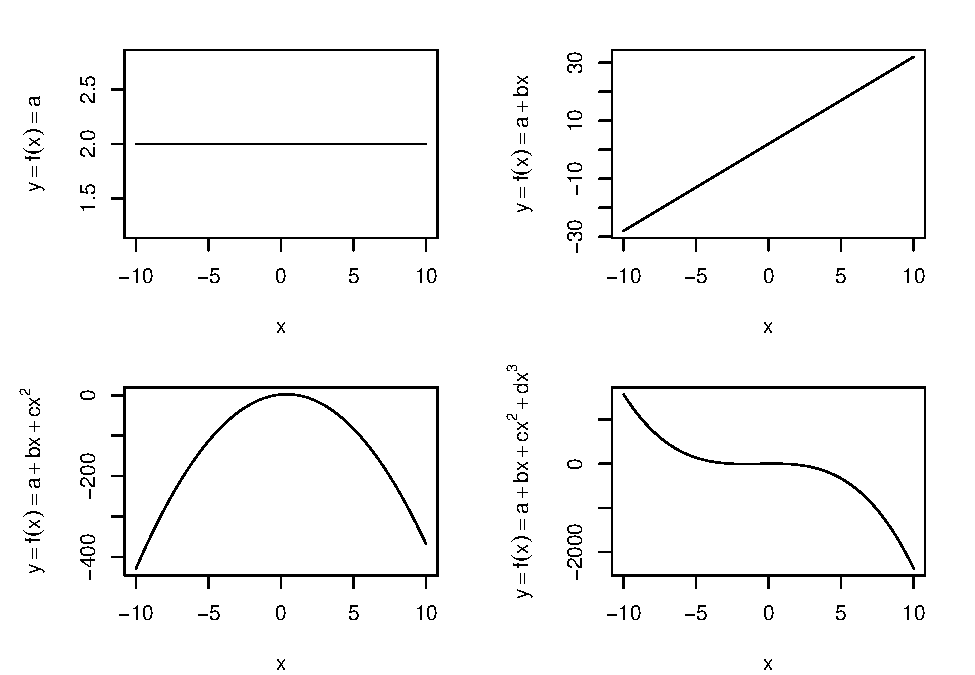
\includegraphics{bookdown-demo_files/figure-latex/fig-3-1-1.pdf}
\caption{\label{fig:fig-3-1}Лінійні та поліноміальні функції \(y = f(x)\) де \(f(x) = a\), \(f(x) = a + bx\), \(f(x) = a + bx + cx^2\), \(f(x) = a + bx + cx^2 + dx^3\) для \(a=2, b = 3, c = -4, d = -2\).}
\end{figure}

Більш поширеними є рівняння прямих ліній, які залежать від змінної \(x\). Найпростішим прикладом буде лінійне рівняння вигляду

\[y = f(x) = a + bx\]

де коефіцієнт \(a\) відповідає значенню \(y\) за \(x = 0\) та коефіцієнт \(b\) відповідає нахилу прямої, тобто відповідає на питання ``на скільки одиниць змінюється \(y\) за зміни \(x\) на одну одиницю''.

Наприклад, розгляньмо детальніше функцію \(y = f(x) = a + bx\), в якій \(a = 2, b = 3\) (Рис. \ref{fig:fig-3-2}):

\begin{figure}
\centering
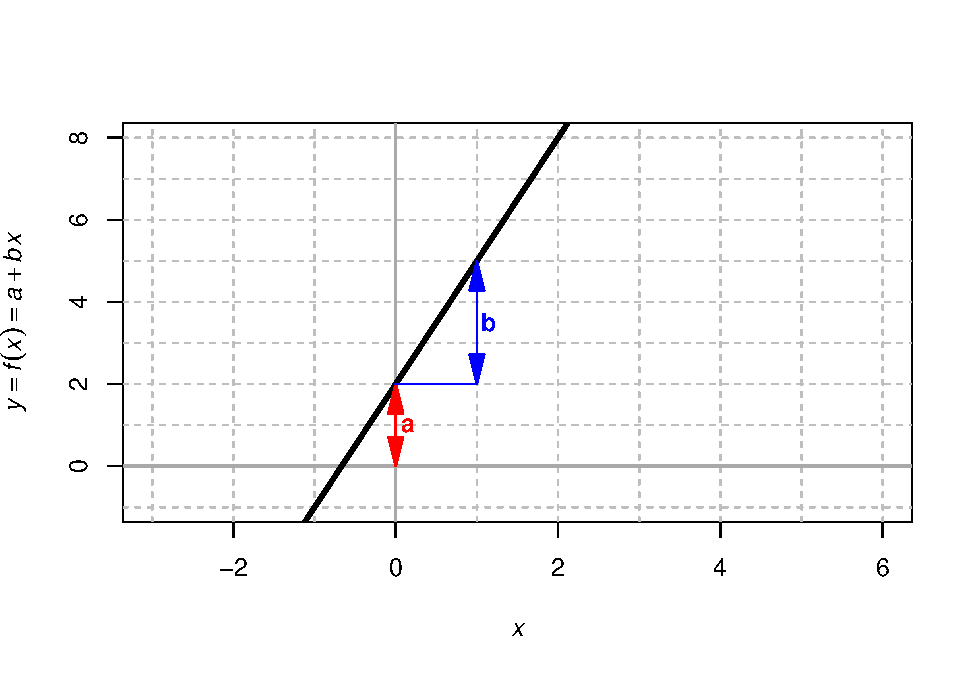
\includegraphics{bookdown-demo_files/figure-latex/fig-3-2-1.pdf}
\caption{\label{fig:fig-3-2}Зміст параметрів лінійної функції \(y = f(x) = a + bx\) для \(a=2, b = 3\).}
\end{figure}

Лінійна функція є окремим випадком поліноміальної функції, в якій ми буквенні коефіцієнти (\(a, b, c, \cdots\)) позначимо через індексовані коефіцієнти (\(\beta_0, \beta_1, \beta_2, \cdots\)):

\[p(x, m) = \beta_0 + \beta_1 x + \beta_2 x^2 + \cdots + \beta_m x^m\]

де \(m\) позначає ступінь полінома. Відтак, найпростіша функція перетину є поліноміальною функцією ступеню \(m = 0\), де \(p(x, m = 0) = \beta_0\), функція прямої є поліноміальною функцією ступеню \(m = 1\), де \(p(x, m = 1) = \beta_0 + \beta_1 x\), квадратична функція є поліноміальною ступеню \(m = 2\), де \(p(x, m = 2) = \beta_0 + \beta_1 x + \beta_2 x^2\) тощо.

Варто зазначити, що \(y\) може бути не лише лінійною функцією однієї змінної, скажімо, \(x\), а й комбінації \(m\) змінних \((x_1, x_2, x_3, \cdots, x_m)\), наприклад,

\[y = f(x_1, x_2, \cdots, x_m) = \beta_0 + \beta_1 x_1 + \beta_2 x_2 + \cdots + \beta_m x_m\]

В статистичному методі лінійної регресії одна зі змінних може являти собою трансформовану іншу змінну. Наприклад, якщо ми визначимо \(x_2\) як \(x_2 = (x_1)^2\), то квадратне рівняння можна визначити як лінійну комбінацію:

\[y = f(x_1, x_2) = \beta_0 + \beta_1 x_1 + \beta_2 x_2 = \beta_0 + \beta_1 x_1 + \beta_2 (x_1^2) = p(x_1, 2)\]

Таким чином, лінійна регресія може бути легко використана для моделювання нелінійних поліноміальних взаємозв'язків за рахунок трансформації змінних і їх використання в лінійних рівняннях.

\subsection{Логарифми}\label{logs}

Логарифмування є зворотним процесом то зведення в ступінь. Логарифм числа \(x\) із основою \(a\) є таким числом, зведення якого до ступеню \(a\) поверне число \(x\), тобто,

\[\log_a x = b\iff a^b = x\]

Найбільш поширеними є десятковий логарифм \(\log_{10}\) та натуральний логарифм \(\log_e\) де \(e\) -- число Ейлера \(e \approx 2.718\), константа, визначена як \(e = \lim\limits_{n \rightarrow \infty} (1 + \frac{1}{n})^n\).

В екології особливо поширений модифікований десятковий логарифм, оскільки чисельності організмів часто мають або низькі значення на кшталт \(0, 1, 2\), або дуже високі значення порядку сотень та тисяч, на рівні яких можна знехтувати одиничними особами\footnote{на рівні однієї, двох, трьох особин плюс-мінус одна особина багато чого змінює, в той час якщо є значення, скажімо, \(1234\), то плюс-мінус одна особина не вносить значної інформації; порівняйте \(\log_{10} 1 = 0\), \(\log_{10} 2 = 0.301\), \(\log_{10} 3 = 0.477\), і \(\log_{10} 1233 = 3.091\), \(\log_{10} 1234 = 3.091\), \(\log_{10} 1235 = 3.092\)}.

Модифікація логарифмічної трансформації в екології побудована таким чином, аби \(0\) відповідало \(0\) особин, \(1\) відповідало \(1\) особині, \(2\) відповідало \(10\) особинам, \(3\) відповідало \(100\) особинам, і так далі (\href{https://doi.org/10.1111/j.1461-0248.2006.00926.x}{Anderson et al.~2006}). Такої трансофрації легко досягнути використовуючи функцію котра враховує факт, що логарифмування від'ємних значень та нуля неможливе (\(\log0 = -\infty\)):

\[f(x) = \begin{cases}
[\log_{10}(x)+1] \times \mathbb{I}_x(x > 0)\\
0 \times \mathbb{I}_x(x = 0)
\end{cases}\]

де \(\mathbb{I}_x(\cdot)\) є індикаторною функцією, котра приймає значення \(1\) якщо логічна умова \((\cdot)\) (тут, що \(x > 0\)) справджується.

Варто мати на увазі, що, в загальному, логарифмічне трансформування чисельностей не є оптимальною практикою, адже різниця між \(\log_{10}(0)\) та \(\log_{10}(1)\) така ж, як, наприклад, між \(\log_{10}(1000)\) та \(\log_{10}(10000)\), в той час як відсутність виду, котра призводить до отримання нульової чисельності, може передбачати набагато важливіші екологічні механізми порівняно із присутністю виду, котра призводить до не-нульової чисельності (\href{https://doi.org/10.1111/j.2041-210X.2010.00021.x}{O'Hara and Kotze 2010}).

Логарифми мають наступні властивості:

\[\log_a(xy) = \log_a(x) + \log_a(y)\]

\[\log_a(\frac{x}{y}) = \log_a(x) - \log_a(y)\]

\[\log_a(x^b) = b \log_a (x)\]

\[\log_a(x) = \frac{\log_b (x)}{\log_b (a)} \forall b\]

\subsection{Поширені математичні функції}\label{ux43fux43eux448ux438ux440ux435ux43dux456-ux43cux430ux442ux435ux43cux430ux442ux438ux447ux43dux456-ux444ux443ux43dux43aux446ux456ux457}

Кількість найпростіших математичних функцій доволі обмежена, однак, їх використання для трансформації змінних може бути кардинально різним. Трансформація даних може знадобитись пізніше, наприклад, для задоволення передбачень певних статистичних методів. Наприклад, лінійна регресія передбачає, що змінні розподілені нормально. В разі, якщо це не відповідає дійсності, одним із варіантів подальших дій є трансформування змінних певною функцією (наприклад, логарифмічно), за чого результуюча змінна може мати ближчий до нормального розподіл. Форми таких функцій наведені на Рис. \ref{fig:fig-3-3}.

\begin{figure}
\centering
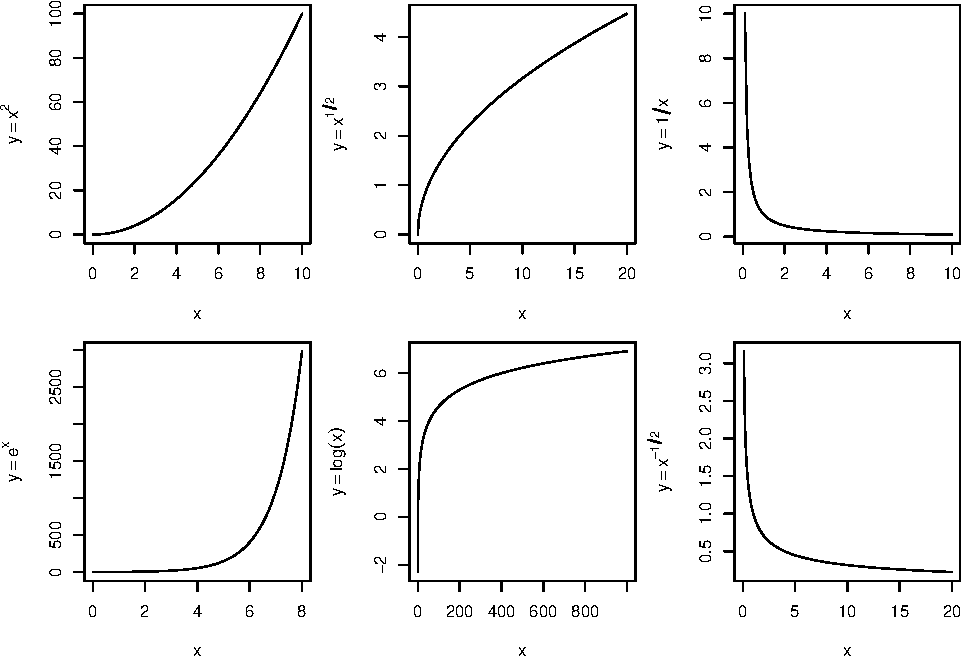
\includegraphics{bookdown-demo_files/figure-latex/fig-3-3-1.pdf}
\caption{\label{fig:fig-3-3}Графіки поширених функцій.}
\end{figure}

Варто також мати на увазі зворотні функції:

\begin{itemize}
\tightlist
\item
  поліноми та корені \(f(x) = x^2 \iff f^{-1}(y) = y^{1/2}\);
\item
  експоненти та логарифми \(f(x) = e^x \iff f^{-1}(y) = \log_e(y)\);
\item
  зворотні функції \(f(x) = 1/x \iff f^{-1}(y) = 1/y\).
\end{itemize}

\subsection{Властивості сум}\label{ux432ux43bux430ux441ux442ux438ux432ux43eux441ux442ux456-ux441ux443ux43c}

Суму позначають як \(\sum\limits_{i=m}^{n}f(x_i)\) де \(i\) є індексом сумації, \(x_i\) -- індексованою змінною, \(m\) -- нижня межа сумації, \(n\) -- верхня межа сумації. В програмуванні таку нотацію можна пояснити через цикл:

\begin{Shaded}
\begin{Highlighting}[]
\FunctionTok{sum}\NormalTok{(}\ControlFlowTok{for}\NormalTok{ (i }\ControlFlowTok{in}\NormalTok{ m}\SpecialCharTok{:}\NormalTok{n)\{}
  \FunctionTok{f}\NormalTok{(x[i])}
\NormalTok{\})}
\end{Highlighting}
\end{Shaded}

Суми мають наступні властивості

\[\sum\limits_{i=m}^{n}c\cdot f(x_i) = c \cdot \sum\limits_{i=m}^{n} f(x_i) \text{ } \forall \text{ } c : \text{const}\]

\[\sum\limits_{i=m}^{n} \left[ f(x_i) + g(x_i)\right] = \sum\limits_{i=m}^{n} f(x_i) + \sum\limits_{i=m}^{n} g(x_i)\]

\[\sum\limits_{i=m}^{n} f(x_i) = \sum\limits_{i=m}^{a} f(x_i) + \sum\limits_{i=a+1}^{n} f(x_i)\]

\[\left( \sum\limits_{i = m}^n x_i \right)\left( \sum\limits_{j = m}^n y_j \right) = \sum\limits_{i = m}^n \sum\limits_{j = m}^n (x_i y_j)\]

\[\sum \limits_{i=1}^n c = nc\]

\[\sum \limits_{i=0}^n \log i = \log n!\]

\[\sum \limits_{i=0}^n \binom{n}{i} = 2^n\]

\[\sum \limits_{i=0}^n \binom{n}{i} a^{n-i} b^i = (a+b)^n\]

\subsection{Властивості добутків}\label{ux432ux43bux430ux441ux442ux438ux432ux43eux441ux442ux456-ux434ux43eux431ux443ux442ux43aux456ux432}

Зміст нотації добутків подібний до суми. Суму позначають як \(\prod\limits_{i=m}^{n}f(x_i)\) де \(i\) є індексом добутку, \(x_i\) -- індексованою змінною, \(m\) -- нижня межа добутку, \(n\) -- верхня межа добутку. Для добутків притаманні наступні властивості:

\[\prod\limits_{i=1}^n x = x^n\]

\[\prod\limits_{i=1}^n x_i y_i = \left( \prod\limits_{i=1}^n x_i\right)\left( \prod\limits_{i=1}^n y_i\right)\]

\[\left( \prod\limits_{i=1}^n x_i \right)^a = \prod\limits_{i=1}^n x_i^a\]

\[\log_b \left[ \prod\limits_{i = m}^n f(x_i) \right] = \sum\limits_{i=m}^n \left[ \log_b f(x_i) \right]\]

\[\prod\limits_{i = m}^n [c \cdot f(x_i)] = c^{\sum_{i=m}^n f(x_i)}\]

\subsection{Диференціювання}\label{ux434ux438ux444ux435ux440ux435ux43dux446ux456ux44eux432ux430ux43dux43dux44f}

Диференціювання функції -- це процес знаходження похідної цієї функції. Похідна функції \(f(x)\) є такою функцією \(f'(x)\), котра описує зміну значення \(f(x)\) за зміни значення аргументу \(x\).

Наприклад, на Рис. \ref{fig:fig-3-2} зображено функцію прямої лінії \(f(x) = 2 + 3x\). В цьому випадку, приріст функції становить 3 одиниці \(y\) на одну одиницю \(x\), і цей приріст залишається незмінним за будь-якого значення \(x\), оскільки функція є прямою. Цей приріст і є похідною, отже, \(f'(x) = 3\).

А що щодо випадків, коли \(f(x)\) не є лінійною, що трапляється набагато частіше? В такому випадку, приріст \(f(x)\) залежить від значення \(x\), тобто \(f'(x)\) теж є функцією із аргументом \(x\). Власне, знаходження цієї функції і є метою диференціювання. Формально, визначення похідної являє собою зміну \(f(x)\) за найменшої різниці \(x\).

Наприклад, визначмо функцію \(f(x) = -5x + x^3\) (Рис. \ref{fig:fig-3-4}):

\begin{figure}
\centering
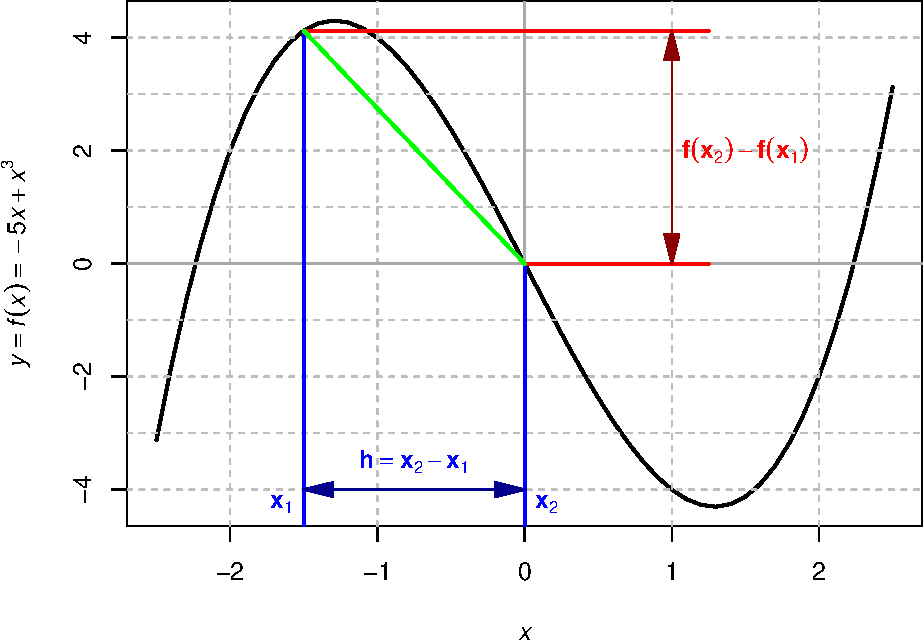
\includegraphics{bookdown-demo_files/figure-latex/fig-3-4-1.pdf}
\caption{\label{fig:fig-3-4}Функція \(f(x) = -5x + x^3\). Приріст цієї функції між \(x_1\) та \(x_2 = x_1 + h\) складає \(\frac{f(x_1 + h) - f(x_1)}{h}\).}
\end{figure}

Для цієї функції, похідна буде такою функцією із аргументом \(x\), котра описуватиме \(f(x_2) - f(x_1)\) на зміну \((x_2 - x_1)\). На Рис. \ref{fig:fig-3-4} показано зміну \(f(x)\) для \(x_2 = 0, x_1 = -1.5\), тобто \(h = x_2 - x_1 = 1.5\), де значення функції становить \(f(x_2) = -5 \cdot 0 + 0^3 = 0\), \(f(x_1) = -5 \cdot (-1.5) + (-1.5)^3 = 4.125\), отже, \(f(x_2) - f(x_1) = f(x_1+h) - f(x_1) = -4.125\), а темп цієї зміни на одиницю \(x\) становить \(\frac{f(x_1 + h) - f(x_1)}{h} = \frac{-4.125}{1.5} = -2.75\).

На тій частині функції, котра відповідає \(x_1, x_1+h\), отримане значення темпу зміни може не цілком відповідати реальній картині. Ми бачимо, що функція трішки зростає після \(x_1\), потім спадає, і взагалі є нелінійною, але обчислене значення \(\frac{f(x_1 + h) - f(x_1)}{h} = \frac{-4.125}{1.5} = 2.75\) відповідає ситуації, коли розглянута функція є прямою лінією (зображено зеленим). Аби відобразити справжню природу зміни значення функції, необхідно зменшити значення \(h\) до найменшого можливого значення. Відтак, класичне визначення похідної -- це така функція із аргументом \(x\), що описує темп зміни \(\frac{f(x+h) - f(x)}{h}\) за найменшої зміни \(h\):

\[f'(x) = \frac{df(x)}{dx} = \lim\limits_{h \rightarrow 0}\frac{f(x+h) - f(x)}{h}\]

де позначення похідної через \(\frac{df(x)}{dx}\) інтуїтивно вказує на її природу, якщо позначити зміну значення змінної через \(d\): зміна значення \(f(x)\) поділена на зміну значення \(x\). Похідну варто сприймати як приріст функції, котрий буде позитивним коли функція зростає, негативним коли функція спадає, і дорівнює нулю коли функція залишається сталою (таке можливе або якщо функція є прямою горизонтальною лінією, або коли в точках перегину, коли функція перестає зростати і починає спадати або навпаки).

Похідні мають наступні властивості, котрі допомагають розрахувати їх для будь-якої неперервної функції:

\[\frac{d}{dx}a = 0\]

\[\frac{d}{dx}ax = a\]

\[\frac{d}{dx} x^a = ax^{a-1}\]

\[\frac{d}{dx} e^x = e^x\]

\[\frac{d}{dx} a^x = a^x \ln (a) \text{ } \forall \text{ } a>0\]

\[\frac{d}{dx} \ln (x) = \frac{1}{x} \text{ } \forall \text{ } x>0\]

\[\frac{d}{dx} \log_a(x) = \frac{1}{x \ln(a)}\]

В диференціюванні складних функцій (функцій, котрі складаються з інших функцій, наприклад, \(f(\cdot)\) і \(g(\cdot)\)) керуються наступними правилами:

\[\frac{d}{dx} \left( af(x) + b g(x) \right) = a \frac{d}{dx}f(x) + b \frac{d}{dx}g(x) \iff (af(x) + bg(x))' = af'(x) + bg'(x)\]

\[\frac{d}{dx}(f(x)g(x)) = \frac{df(x)}{dx} g(x) + f(x) \frac{dg(x)}{dx} \iff (f(x)g(x))' = f'(x)g(x) + f(x)g'(x)\]

\[\frac{d}{dx} \left( \frac{f(x)}{g(x)}\right) = \frac{\frac{df(x)}{dx}g(x) - f(x) \frac{dg(x)}{dx}}{g(g(x))} \iff \left( \frac{f(x)}{g(x)} \right)' = \frac{f'(x)g(x) - f(x)g'(x)}{g^2(x)}\]

і для функції функції \(f(x) = h(g(x))\),

\[\frac{df(x)}{dx} = \frac{dh(g(x))}{dg(x)} \cdot \frac{dg(x)}{dx} \iff f'(x) = h'(g(x)) \cdot g'(x)\]

Оскільки похідна є функцією сама по собі, її також можна диференціювати (тобто знайти \(n\)-ну похідну, або похідну \(n\)-ного порядку). Наприклад, для функції \(f(x) = -5x + x^3\),

\[\begin{cases}
\frac{d}{dx}f(x) = -5 + 3x^2 \\
\frac{d^2}{dx}f(x) = 6x \\
\frac{d^3}{dx}f(x) = 6 \\
\frac{d^4}{dx}f(x) = 0
\end{cases}\]

\begin{figure}
\centering
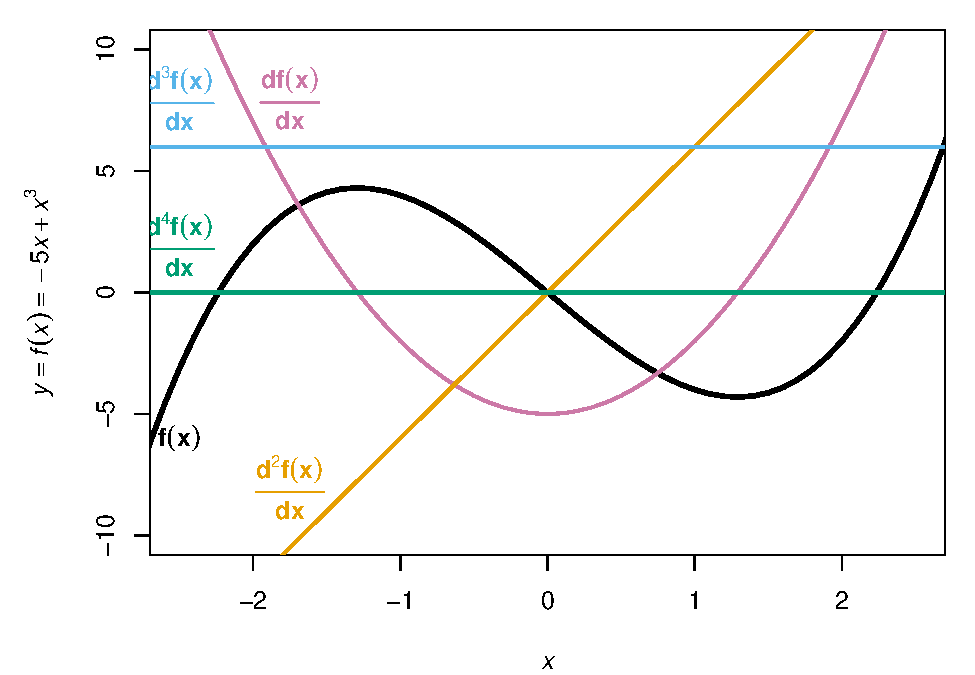
\includegraphics{bookdown-demo_files/figure-latex/fig-3-5-1.pdf}
\caption{\label{fig:fig-3-5}Функція \(f(x) = -5x + x^3\) та її похідні.}
\end{figure}

\subsection{Інтегрування}\label{ux456ux43dux442ux435ux433ux440ux443ux432ux430ux43dux43dux44f}

Інтегрування функції \(f(x)\) -- це процес знаходження такої функції \(F(x)\), похідна якої являє собою функцію \(f(x)\):

\[\frac{d}{dx}F(x) = f(x) \iff \int f(x) dx = F(x) + C\]

де \(C\) -- це будь-яка константа (оскільки похідна константи дорівнює нулю, ця константа не впливає на результат диференціювання).

Інтеграл є, певною мірою, континуальний аналог суми: якщо означення суми оперує дискретними значеннями \(i: i = 1, 2, 3, \cdots, n\), то інтеграл, подібно до похідних, розраховується для найменших можливих інтервалів аргументу функції \(x\).

\textbf{\emph{Невизначений інтеграл}} функції \(f(x)\) \(\int f(x)dx = F(x)\) має зміст як функція, похідна якої дорівнює вихідній функції \(f(x)\). Водночас, \textbf{\emph{визначений інтеграл}} \(\int\limits_a^b f(x) dx = F(b) - F(a)\) часто використовується для знаходження площі під кривою \(f(x)\), що обмежена значеннями \(a\) і \(b\).

В разі, якщо аналітичне знаходження невизначеного інтегралу складне або неможливе, корисним може видатись Рейманівське визначення визначеного інтегралу:

\[\int\limits_a^b f(x) dx = F(a) - F(b) = \sum\limits_{i=1}^n [F(x_i) - F(x_{i-1})]\]

де \([F(x_i) - F(x_{i-1})]\) є площею прямокутника, обмеженого функцією \(f(x)\) і дуже маленьким інтервалом \([x_{i-1}, x_i)\) (Рис. \ref{fig:fig-3-6}).

\begin{figure}
\centering
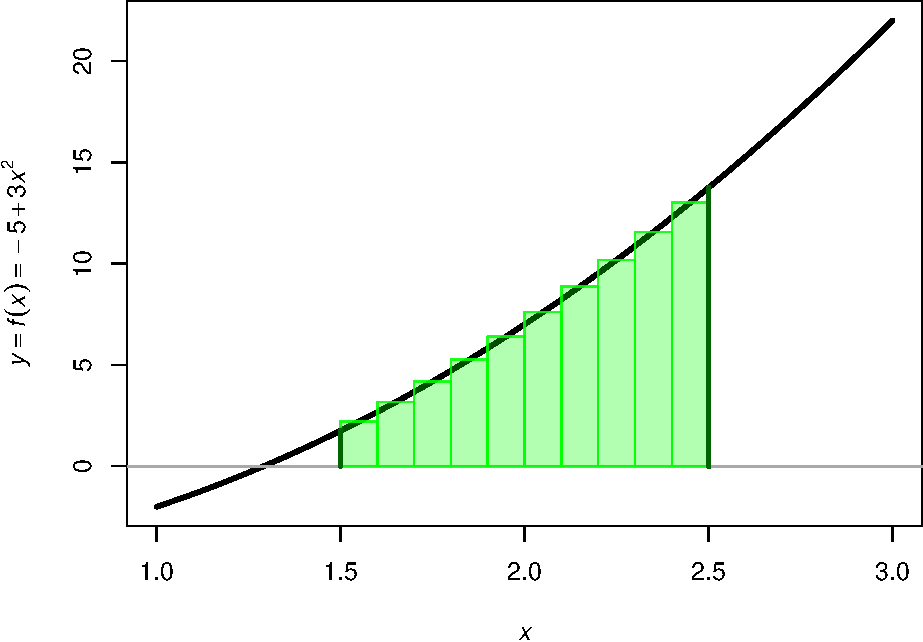
\includegraphics{bookdown-demo_files/figure-latex/fig-3-6-1.pdf}
\caption{\label{fig:fig-3-6}Знаходження визначеного інтеграла як Рейманівську суму функції \(f(x) = -5 + 3x^2\).}
\end{figure}

Якщо, наприклад, шукати площу під кривою як на Рис. \ref{fig:fig-3-6} поділом інтервалу між \(a = 1.5\), \(b = 2.5\) на \(10\) прямокутників (хоча їх може бути скільки завгодно), то це нескладно обчислити за допомогою R:

\begin{Shaded}
\begin{Highlighting}[]
\NormalTok{f }\OtherTok{\textless{}{-}} \ControlFlowTok{function}\NormalTok{(x) }\SpecialCharTok{{-}}\DecValTok{5} \SpecialCharTok{+} \DecValTok{3}\SpecialCharTok{*}\NormalTok{x}\SpecialCharTok{\^{}}\DecValTok{2}
\FunctionTok{sum}\NormalTok{(}\FunctionTok{sapply}\NormalTok{(}\FunctionTok{seq}\NormalTok{(}\FloatTok{1.5}\NormalTok{, }\FloatTok{2.4}\NormalTok{, }\FloatTok{0.1}\NormalTok{)}\SpecialCharTok{+}\FloatTok{0.05}\NormalTok{, }\ControlFlowTok{function}\NormalTok{(x) }\FloatTok{0.1}\SpecialCharTok{*}\FunctionTok{f}\NormalTok{(x)))}
\end{Highlighting}
\end{Shaded}

\begin{verbatim}
## [1] 7.2475
\end{verbatim}

Із прикладу на Рис. \ref{fig:fig-3-5} ми знаємо, що функція \(f(x) = -5 + 3x^2\) є першою похідною функції \(F(x) = -5x + x^3\), яка, за визначенням, є невизначеним інтегралом \(\int f(x)dx\). Відповідно,

\[
\begin{aligned}
  \int\limits_{1.5}^{2.5}-5 + 3x^2 dx = F(2.5) - F(1.5) = \left[ -5x + x^3 \right]_{1.5}^{2.5} = \\ [-5 \cdot 2.5 + 2.5^3] - [-5 \cdot 1.5 + 1.5^3] = 3.125 - (-4.125) = 7.25 \simeq 7.2475
\end{aligned}
\]

Типові інтеграли мають наступні значення:

\[\int x^a dx = \frac{x^{a+1}}{a+1} + C \text{ } \forall \text{ } a \neq -1\]

\[\int x^{-1} dx = \int \frac{dx}{x} = \ln(|x|) + C\]

\[\int axdx = ax + C\]

\[\int \frac{1}{ax + b}dx = \frac{1}{a} \ln(|ax+b|) + C\]

\[\int \ln(x) dx = x \ln(x) -x + C\]

\[\int e^x dx = e^x + C\]

Інтегралам притаманні наступні властивості:

\[\int \limits_a^b c f(x) dx = c \int \limits_a^b f(x) dx\]

\[\int \limits_a^b f(x) + g(x) dx = \int \limits_a^b f(x) dx + \int \limits_a^b g(x) dx\]

\[\int \limits_a^a f(x)dx = 0\]

\[\int \limits_a^b f(x)dx = -\int \limits_b^a f(x)dx\]

\[\int \limits_a^c f(x)dx = \int \limits_a^b f(x)dx + \int \limits_b^c f(x)dx \text{ } \forall \text{ } a < b < c\]

Для інтегрування складних функцій використовують наступні техніки:

\begin{itemize}
\tightlist
\item
  інтегрування підстановкою
\end{itemize}

\[\int \limits_a^b f(g(x)) g'(x)dx = \int \limits_{g(a)}^{g(b)} f(u) du\]

де \(u = g(x)\), \(du = g'(x)dx\)

\begin{itemize}
\tightlist
\item
  інтегрування частинами
\end{itemize}

\[\int u (dv) = uv - \int v (du) \iff \int f(x)g'(x)dx = f(x)g(x) - \int f'(x) g(x) dx\]

де \(v = \int dv\).

В цілому, в екології рідко коли потрібно аналітично вирішити інтеграл чи похідну, однак, розуміння \emph{змісту} цих операцій необхідне для подальшого розуміння статистичних підходів. В рідкісних випадках, коли необхідно вирішити певний інтеграл, має сенс скористатися онлайн-сервісами на кшталт \href{https://www.integral-calculator.com/}{integral-calculator.com} або розрахувати значення визначеного інтегралу ітеративно за допомогою Рейманівської суми, як показано вище. Варто також мати на увазі, що деякі функції неможливо або дуже складно проінтегрувати.

\section{Лінійна алгебра}\label{matrices}

\subsection{Визначення матриці}\label{ux432ux438ux437ux43dux430ux447ux435ux43dux43dux44f-ux43cux430ux442ux440ux438ux446ux456}

Матриця є двовимірним набором значень, що позначається як

\[\textbf{A} = \begin{bmatrix}
a_{1, 1} & a_{1,2} & \cdots & a_{1, n}\\
a_{2, 1} & a_{2,2} & \cdots & a_{2, n}\\
\vdots & \vdots & a_{i,j} & \vdots \\
a_{m, 1} & a_{m,2} & \cdots & a_{m, n}
\end{bmatrix}\]

в якій \(i: 1, 2, \cdots, m-1, m\) позначає індекс рядка елементу і \(j: 1, 2, \cdots, n-1, n\) позначає індекс колонки елементу \(a_{i, j}\). В цій книзі матриці як об'єкти позначатимуться жирними великими літерами і визначатимуться як матриці в квадратних дужках, але варто мати на увазі, що позначення іноді варіюють в різних джерелах.

Розмірність матриці визначається кількістю рядків \(m\) та кількістю колонок \(n\). Якщо один із цих вимірів дорівнює одиниці, матриця являє собою \textbf{\emph{вектор}} -- послідовність значень. Поняття вектору важливе для розуміння оперування даними, адже спостереження (рядки) та параметри (колонки) в масиві даних є векторами розмірністю \(m \times 1\) або \(1 \times n\). Вектори позначаються як \(\vec{a}\).

В подальшому матриці визначені як жирні літери (напр., \(\mathbf{A}\)), а елементи матриці -- як індексовані літери \(a_{i,j}\), або \([\mathbf{A}]_{i,j}\).

\subsection{Трансформації матриць}\label{ux442ux440ux430ux43dux441ux444ux43eux440ux43cux430ux446ux456ux457-ux43cux430ux442ux440ux438ux446ux44c}

\textbf{\emph{Додавання матриць}}, якащо обидві матриці мають ідентичну розмірність, є доволі очевидним, адже додаються елементи із ідентичними індксами. Наприклад, \(\mathbf{A}+\mathbf{B} = a_{i,j}+b_{i, j}\).

Наприклад, якщо

\[\mathbf{A} = \begin{bmatrix}
a_{1, 1} & a_{1,2} & \cdots & a_{1, n}\\
a_{2, 1} & a_{2,2} & \cdots & a_{2, n}\\
\vdots & \vdots & a_{i,j} & \vdots \\
a_{m, 1} & a_{m,2} & \cdots & a_{m, n}
\end{bmatrix},
\mathbf{B} = \begin{bmatrix}
b_{1, 1} & b_{1,2} & \cdots & b_{1, n}\\
b_{2, 1} & b_{2,2} & \cdots & b_{2, n}\\
\vdots & \vdots & b_{i,j} & \vdots \\
b_{m, 1} & b_{m,2} & \cdots & b_{m, n}
\end{bmatrix}\]

тоді

\[\mathbf{A} + \mathbf{B} = \begin{bmatrix}
a_{1, 1}+b_{1, 1} & a_{1,2}+b_{1,2} & \cdots & a_{1, n}+b_{1, n}\\
a_{2, 1}+b_{2, 1} & a_{2,2}+b_{2,2} & \cdots & a_{2, n}+b_{2, n}\\
\vdots & \vdots & a_{i,j}+b_{i,j} & \vdots \\
a_{m, 1}+b_{m, 1} & a_{m,2}+b_{m,2} & \cdots & a_{m, n}+b_{m, n}
\end{bmatrix}\]

Подібно до додавання, \textbf{\emph{скалярне множення}} матриць полягає в отриманні добутку константи із кожним елементом матриці:

\[c \cdot \mathbf{A} = c \cdot a_{i, j} = \begin{bmatrix}
c \cdot a_{1, 1} & c \cdot a_{1,2} & \cdots & c \cdot a_{1, n}\\
c \cdot a_{2, 1} & c \cdot  a_{2,2} & \cdots & c \cdot a_{2, n}\\
\vdots & \vdots & c \cdot a_{i,j} & \vdots \\
c \cdot a_{m, 1} & c \cdot a_{m,2} & \cdots & c \cdot a_{m, n}
\end{bmatrix}\]

Нарешті, \textbf{\emph{транспонування}} матриці полягає в заміні індексування рядків та колонки і навпаки, \(i \rightarrow j, j \rightarrow i\), тобто,

\[\mathbf{A'} = \mathbf{A^T} = a'_{j, i} \text{ } \forall \text{ } \mathbf{A} = a_{i, j}\]

\subsection{Операції над матрицями}\label{ux43eux43fux435ux440ux430ux446ux456ux457-ux43dux430ux434-ux43cux430ux442ux440ux438ux446ux44fux43cux438}

\textbf{\emph{Множення матриць}} є дещо складнішим, і загальним правилом є те, що для матриць \(A\) розміром \(m \times n\) і \(B\) розміром \(n \times p\) добуток складатиме матрицю розміром \(m \times p\) із елементами, що відповідають сумі добутків рядків \(A\) та колонок \(B\), тобто елемент добутку матриць із індексами \(i, j\) складатиме (\href{https://books.google.com/books/about/Linear_Algebra.html?id=P8BZzAEACAAJ}{Bogacki 2019}) (Рис. \ref{fig:fig-3-7})

\[[\mathbf{AB}]_{i, j} = \sum \limits_{r=1}^n (a_{i,r} b_{r, j}) = a_{i,1} b_{1, j} + a_{i, 2}b_{2, j} + \cdots + a_{i, n}b_{n, j}\]

\begin{figure}
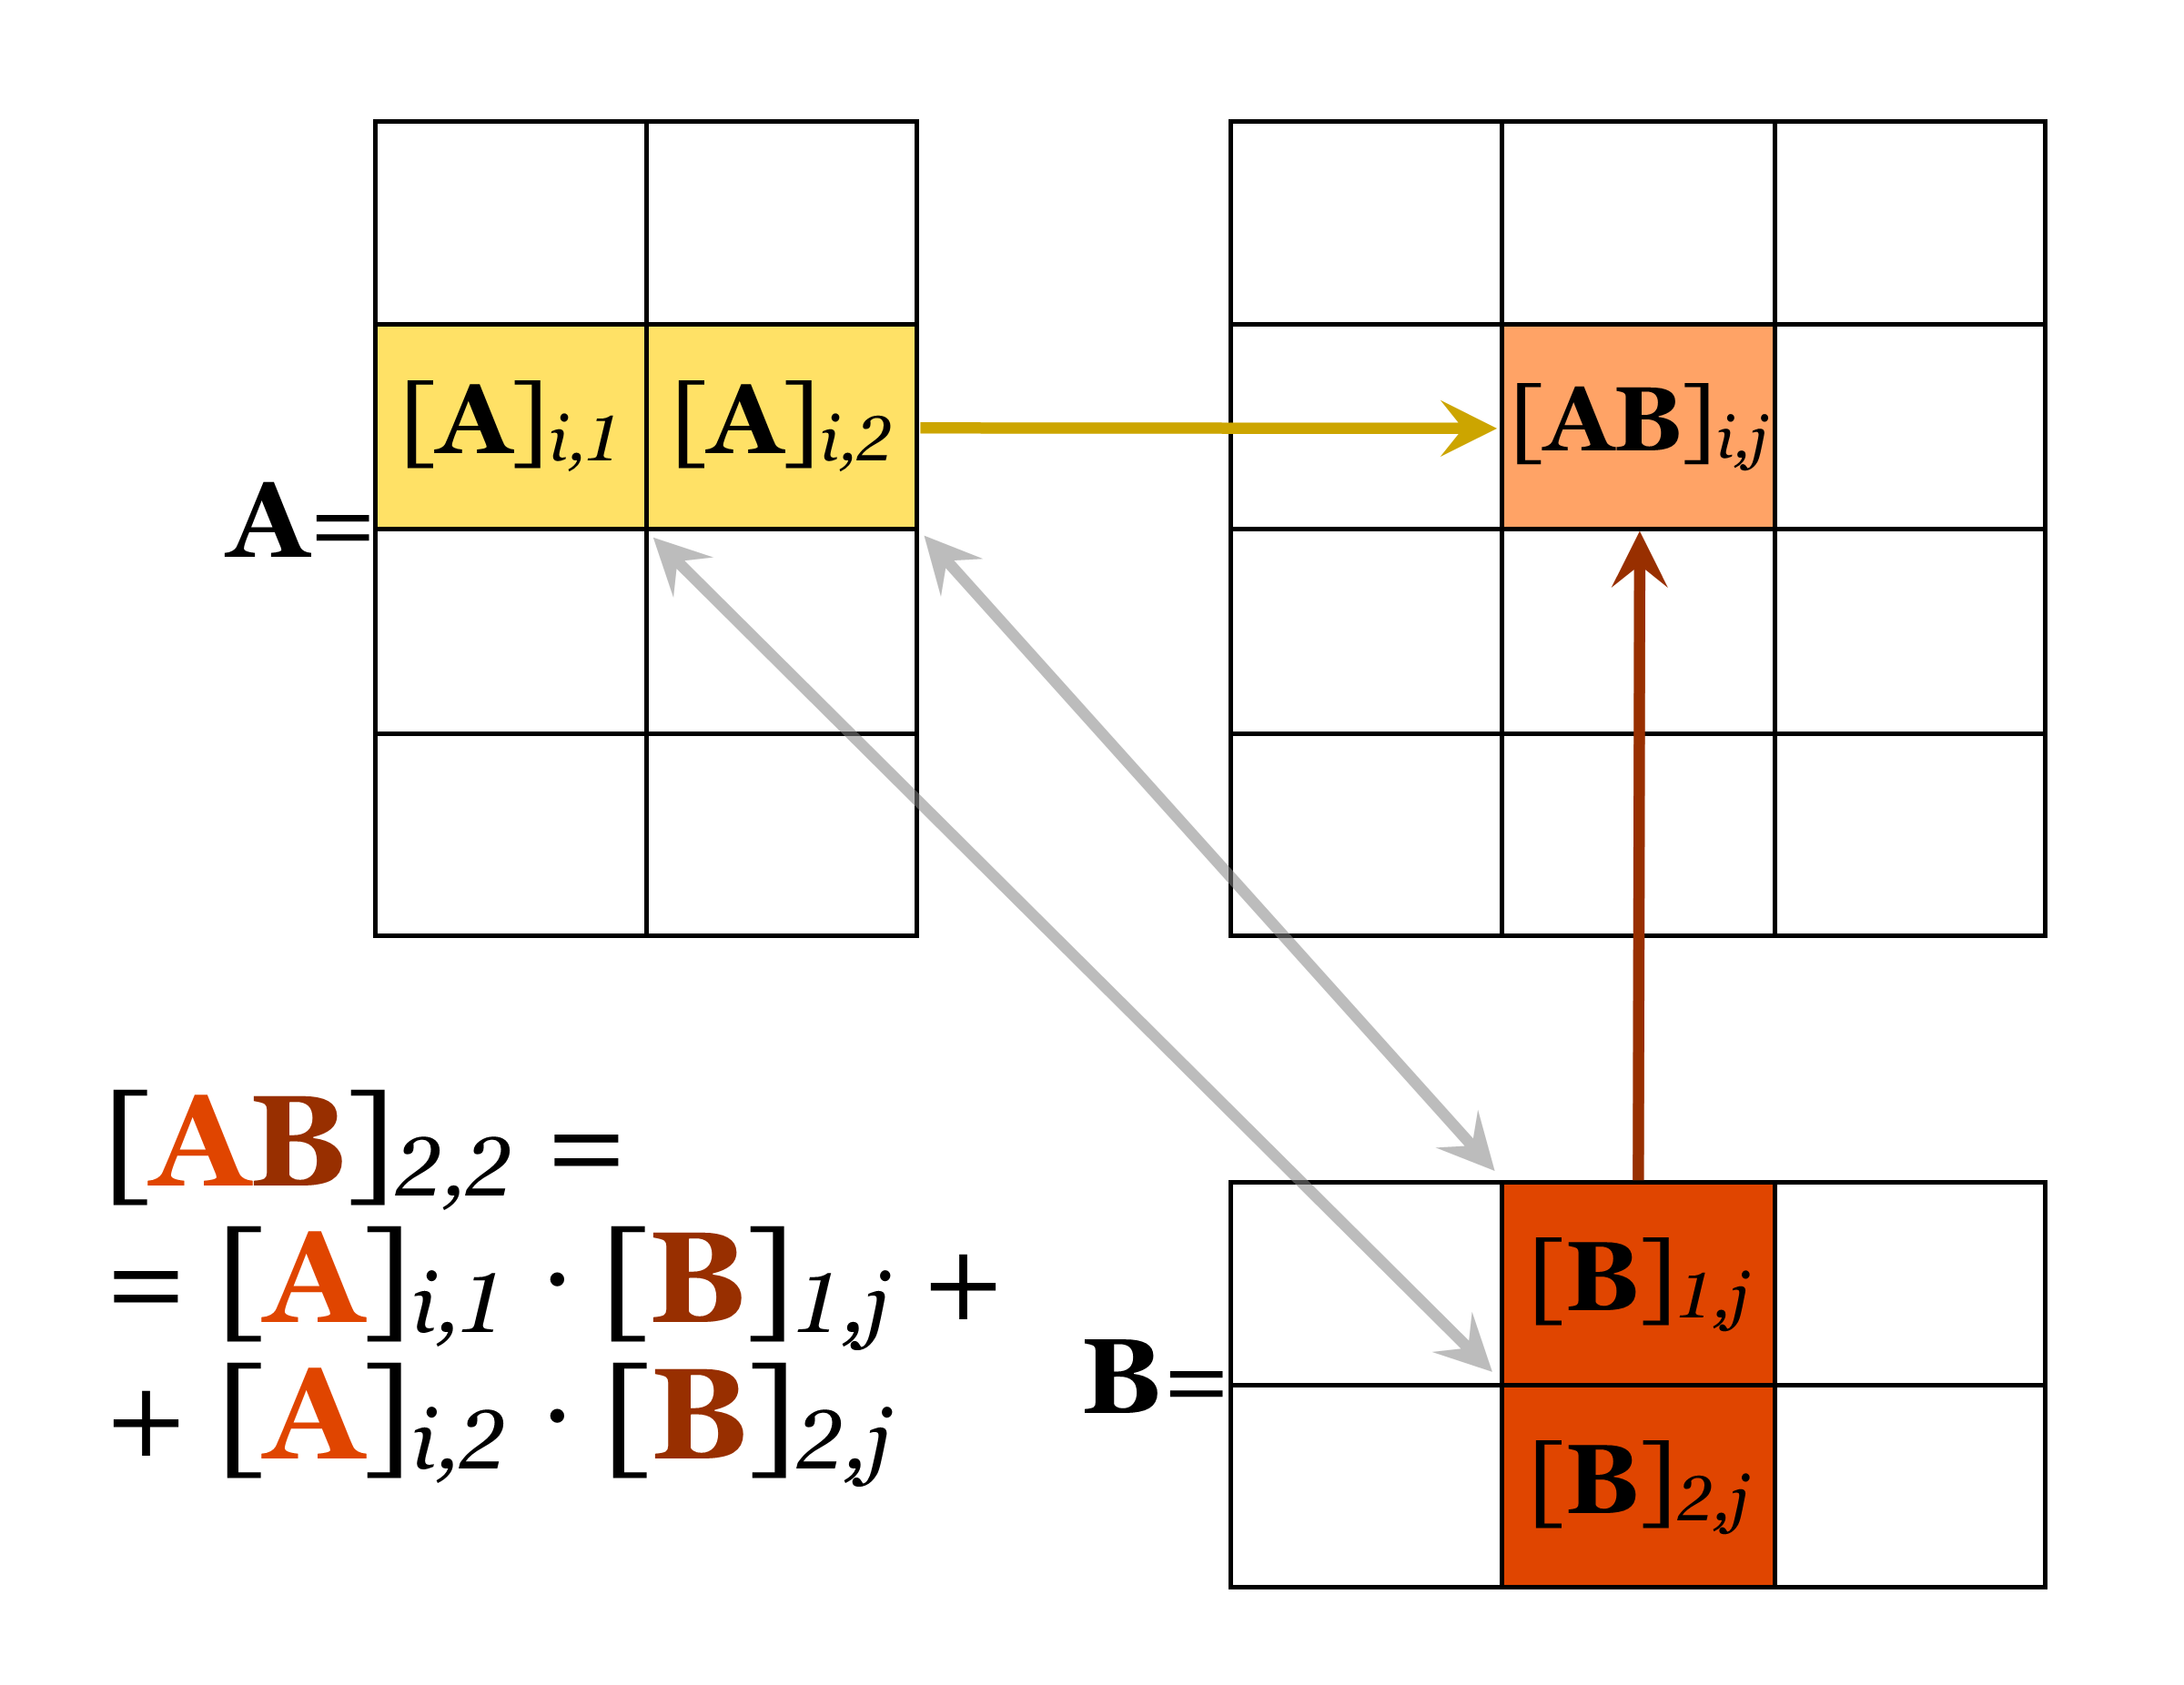
\includegraphics[width=33.33in]{images/matrices} \caption{Знаходження значення елементу добутку матриць $\mathbf{A}$ і $\mathbf{B}$.}\label{fig:fig-3-7}
\end{figure}

Для добутків матриць властиво, що

\[\mathbf{AB} \neq \mathbf{BA}\]

\[(\mathbf{AB})\mathbf{C} = \mathbf{A}(\mathbf{BC})\]

\[(\mathbf{A+B})\mathbf{C} = \mathbf{AC} + \mathbf{BC}\]

\[\mathbf{C}(\mathbf{A+B}) = \mathbf{CA} + \mathbf{CB}\]

Очевидно, що якщо множення матриць можливе, то можливо також і звести матрицю в ступінь, наприклад,

\[\mathbf{A}^3 = (\mathbf{AA})\mathbf{A}\]

Уявімо квадратну \textbf{\emph{одиничну матрицю}} \(\mathbf{I}_n\) розміром \(n \times n\), де

\[\mathbf{I}_n = \begin{bmatrix}
1 & 0 & 0 & \cdots & 0\\
0 & 1 & 0 & \cdots & 0\\
0 & 0 & 1 & \cdots & 0\\
\vdots & \vdots & \vdots & \ddots  &\vdots \\
0 & 0 & 0 & \cdots & 1
\end{bmatrix}\]

тобто всі, крім діагональних, елементи матриці дорівнюють нулю. Тоді

\[\mathbf{AB} = \mathbf{I}_n = \mathbf{BA}\]

отже, \(\mathbf{B}\) є \textbf{\emph{оберненою матрицею}} \(\mathbf{A}\):

\[\mathbf{B} = \mathbf{A}^{-1}\]

\[\mathbf{AA^{-1}} = \mathbf{I}_n\]

\[\mathbf{A}^0 = \mathbf{I}_n\]

Очевидно, що \textbf{не} для будь-якої матриці може існувати обернена матриця.

Подібно до математичних функцій, \textbf{\emph{лінійні трансформації}} можуть приймати вектори чи матриці в якості аргументу:

\[F: \mathbb{R}^n \rightarrow \mathbb{R}^m \text{ якщо}\]

\[F(\vec{u} + \vec{v}) = F(\vec{u}) + F(\vec{v}) \text{ } \forall \text{ } \vec{u}, \vec{v}\]

\[F(c \vec{u}) = c F(\vec{u}) \text{ } \forall \text{ } \vec{u}, c\]

\[F(c_1 \vec{u_1} + \cdots + c_k \vec{u_k}) = c_1 F(\vec{u_1}) + \cdots + c_k F(\vec{u_k})\]

\[F: \mathbb{R}^n \rightarrow \mathbb{R}^m \iff \exists \mathbf{A}: F(\vec{v}) = \mathbf{A} \vec{v}, \mathbf{A} = a_{i, j}, 1 < i<m, 1 < j < n\]

\subsection{Детермінант, власні вектори, та власне значення}\label{ux434ux435ux442ux435ux440ux43cux456ux43dux430ux43dux442-ux432ux43bux430ux441ux43dux456-ux432ux435ux43aux442ux43eux440ux438-ux442ux430-ux432ux43bux430ux441ux43dux435-ux437ux43dux430ux447ux435ux43dux43dux44f}

\textbf{\emph{Детермінант}} визначається (\href{https://books.google.com/books/about/Linear_Algebra.html?id=P8BZzAEACAAJ}{Bogacki 2019}) для матриці \(1 \times 1\) \(\mathbf{A} = [a_{1, 1}]\) як

\[\det \mathbf{A} = a_{1, 1}\]

і для більших квадратних матриць розміром \(n \times n\) рекурсивно

\[\det \mathbf{A} = \sum \limits_{j=1}^n (-1)^{1+j} a_{1, j} \det \mathbf{M}_{1,j}\]

де \(\mathbf{M}_{i,j}\) є підматрицею від \(\mathbf{A}\) розміром \((n - 1) \times (m - 1)\) із видаленими рядком \(i\) і колонкою \(j\), тобто,

\[\det \mathbf{A} = a_{1,1} \det \mathbf{M}_{1,1} - a_{1,2} \det \mathbf{M}_{1,2} + a_{1,3} \det \mathbf{M}_{1,3} - \cdots + (-1)^{1+n} a_{1, n} \det \mathbf{M}_{1,n}\]

Для матриці \(\mathbf{A}\) розміром \(2 \times 2\), наприклад,

\[\det \mathbf{A} = \det \begin{bmatrix}
a_{1, 1} & a_{1, 2} \\
a_{2, 1} & a_{2, 2}
\end{bmatrix} = a_{1, 1} \cdot a_{2, 2} - a_{1, 2} \cdot a_{2, 1}\]

\subsection{Геометричний зміст матриць}\label{matrices_art}

Технічні визначення операцій над матрицями можуть видаватись надмірно деталізованими і неінтуїтивними правилами, котрі просто необхідно завчити. Однак, всі ці правила мають очевидний геометричний зміст, котрий рідко використовують в поясненнях базової теорії матриць \href{https://youtube.com/playlist?list=PLZHQObOWTQDPD3MizzM2xVFitgF8hE_ab}{3Blue1Brown 2023}.

В першу чергу, необхідно зрозуміти поняття вектора. В багатьох чисельних методах і, зокрема, в програмному середовищі R, векторами звуться скінченні ряди чисел, наприклад, змінна в наборі даних. Однак, зі шкільної програми математики можна пригадати, що векторами є і спрямовані відрізки. Наприклад, якщо позначити вектор \(\vec{a}\) як \(\vec{a} = (1, 2)\), то ряд чисел \((1, 2)\) можна зобразити як такий вектор, що починається з координат \((x_0 = 0, y_0 = 0)\) і закінчується координатами \((x_1 = 1, y_1 = 2)\).

Уявімо простір таких векторів. З попереднього параграфу можна помітити, що хоча й, формально, вектор має дві точки (в двовимріному просторі це \((x_0, y_0)\) та \((x_1, y_1)\)), для кожного вектору одна з точок буде однаковою: \((x_0 = 0, y_0 = 0)\). Відтак, ми не втратимо ніякої інформації, якщо для багатьох векторів ми забудемо про початкові точки і визначимо лише кінцеві точки. У двовимірному просторі можна визначити скільки завгодно векторів/точок \(\vec{v_1} = (x_{1, 1}, y_{1, 1}), \vec{v_2} = (x_{1, 2}, y_{1, 2}), \cdots, \vec{v_i} = (x_{1, i}, y_{1, i})\), але, звісно, це справджуватиметься і для одного виміру (\(\vec{v_1} = (x_{1, 1}), \vec{v_2} = (x_{1, 2}), \cdots, \vec{v_i} = (x_{1, i})\)), і для трьох вимірів (\(\vec{v_1} = (x_{1, 1}, y_{1, 1}, z_{1, 1}), \vec{v_2} = (x_{1, 2}, y_{1, 2}, z_{1, 2}), \cdots, \vec{v_i} = (x_{1, i}, y_{1, i}, z_{1, i})\)), і для будь-якої скінченної кількості вимірів. В структурі даних, відтак, хоча й ряди чисел є векторами, ми можемо уявити кожне спостереження як точку у просторі параметрів цього спостереження (т. зв. точка даних, або data point, що ж еквівалентним одиночному спостереженню).

Для простору векторів, матриця є лінійною трансформацією. Тобто, якщо помножити координати точки (або вектору, що є тим самим) на матрицю, то на виході ми отримаємо інший лінійний вектор. Подібно до математичної функції, ми можемо застосувати лінійну трансформацію до всього простору, і отримаємо інший простір, в котрому точки знаходяться та пропорційній до вихідного простору відстані одна від одної, а прямі між точками залишаються прямими\footnote{очевидно, ці дві умови не завжди можуть справджуватися, у випадку чого трансформація не є лінійною}.

Пригадаймо правила множення матриць. Для цього потрібно кожен вектор уявити у вигляді матриці. Наприклад, для вектору \[\vec{a} = (x_1 = 1, y_1 = 2) = \begin{bmatrix} 
x_1 = 1 \\ 
y_1 = 2 \end{bmatrix} = \begin{bmatrix}
1 \\
2 \end{bmatrix}\]

застосуймо матрицю

\[\mathbf{A} = \begin{bmatrix}
1 & 2 \\
3 & 4
\end{bmatrix}\]

\[
\mathbf{A} \vec{a} = \begin{bmatrix}
1 & 2 \\
3 & 4
\end{bmatrix} \cdot \begin{bmatrix}
1 \\ 2 
\end{bmatrix}= \begin{bmatrix}
1 \cdot 1 + 2 \cdot 2 \\
1 \cdot 3 + 2 \cdot 4
\end{bmatrix} = \begin{bmatrix}
5 \\ 11
\end{bmatrix}
\]

Тобто після застосування лінійної трансформації до вектору ми отримуємо вектор такої ж розмірності, при чому ця лінійна трансформація може бути застосована для будь-якого вектору такої розмірності. Тож матриця \(\mathbf{A}\) відповідає лінійній трансформації, зображеній на Рис. \ref{fig:fig-3-8}.

\begin{figure}
\centering
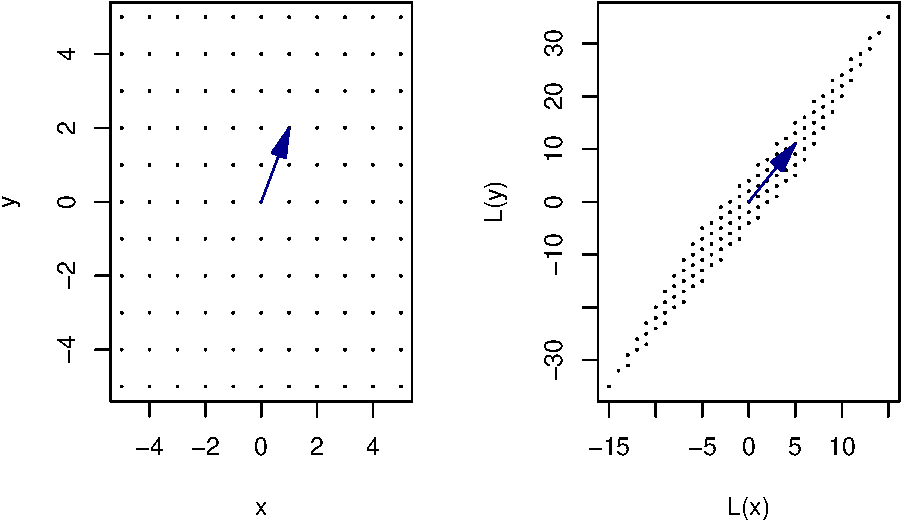
\includegraphics{bookdown-demo_files/figure-latex/fig-3-8-1.pdf}
\caption{\label{fig:fig-3-8}Матриця \(\mathbf{A} = \begin{bmatrix} 1 & 2 \\ 3 & 4 \end{bmatrix}\) як лінійна трансформація простору. Вектор \(\vec{a} = \begin{bmatrix} 1 \\ 2 \end{bmatrix}\) є лише частиною цього простору.}
\end{figure}

Загалом, для всякого двовимірного простору можна уявити два незалежні базові вектори: \(\hat{i} = \begin{bmatrix} 1 \\ 0 \end{bmatrix}\) й \(\hat{j} = \begin{bmatrix} 0 \\ 1 \end{bmatrix}\). Тоді будь-який вектор \(\vec{v}\) є сумою векторів, що відображають добутки певної константи \(a\) та \(\hat{i}\) й \(b\) та \(\hat{j}\): \(\vec{v} = a \hat{i} + b \hat{j}\), а, відтак, всяку лінійну трансформацію \(L(\cdot)\) можна виразити у вигляді \[L(\vec{v}) = a L(\hat{i}) + b L(\hat{j})\]

відтак, лінійна трансформація вектору \(\begin{bmatrix} x \\ y \end{bmatrix} \rightarrow L \left( \begin{bmatrix} x \\ y \end{bmatrix} \right)\) є тотожною лінійній трансформації базових векторів, шкалованих на певні константи для базових векторів:

\[L \left( \begin{bmatrix} x \\ y \end{bmatrix} \right) = x[L (\hat{i})] + y[L(\hat{j})] = \begin{bmatrix} x L(1) & xL(0) \\ y L(0) & y L(1) \end{bmatrix}\]

Тобто сутність квадратної матриці як репрезентації лінійної трансформації -- це сукупність координат, на які припадають базові вектори після лінійної трансформації. Для попереденього прикладу \(\mathbf{A} = \begin{bmatrix} 1 & 2 \\ 3 & 4 \end{bmatrix}\), зокрема, \(L(\hat{i})\) матиме координати \((1, 3)\), а \(L(\hat{j})\) -- \((2, 4)\).

Якщо розглядати матрицю як носій інформації про лінійну трансформацію, то множення матриць є нічим іншим, як застосуванням лінійної трансформації до лінійної трансформації. Тобто, якщо уявити дві лінійні трансформації \(L_1\) та \(L_2\) такі що

\[L_2 \left( L_1 \left( \begin{bmatrix} 
x \\ 
y 
\end{bmatrix} \right) \right) = 
\begin{bmatrix} 
a & c \\ 
b & d
\end{bmatrix}
\left( 
\begin{bmatrix} 
e & g \\ 
f & h
\end{bmatrix}
\begin{bmatrix} 
x \\ 
y 
\end{bmatrix}
\right) = 
\left( 
\begin{bmatrix} 
a & c \\ 
b & d
\end{bmatrix}
\begin{bmatrix} 
e & g \\ 
f & h
\end{bmatrix}
\right)
\begin{bmatrix} 
x \\ 
y 
\end{bmatrix} = 
\begin{bmatrix} 
ae + bg & af + bh \\ 
ce + dg & cf + dh
\end{bmatrix}
\begin{bmatrix} 
x \\ 
y 
\end{bmatrix}\]

Із рисунку \ref{fig:fig-3-8} можна помітити, що площа фігур в просторі змінюється в результаті лінійної трансформації. Детермінант матриці відображає зміну площі квадрата зі сторонами \(\hat{i}\) та \(\hat{j}\) таким чином, що \(A[L(\hat{i} \times \hat{j})] = c \cdot A[(\hat{i} \times \hat{j})]\). Якщо \(c = 0\), то матриця з таким детермінантом позначає лінійну трансформацію, що призводить до зменшення розмірності вектора, а якщо \(c<0\), то (подібно до того, як від'ємна площа має сенс в інтегруванні) змінюється орієнтація \(\hat{i}\) відносно \(\hat{j}\).

Іншим поширеним застосуванням матриць є вирішення квадратних рівнянь. Наприклад, систему вигляду

\[\begin{cases}
a_1 x + b_1 y + c_1 z = d_1 \\
a_2 x + b_2 y + c_2 z = d_2 \\
a_3 x + b_3 y + c_3 z = d_3
\end{cases}\]

можна зобразити у вигляді матриць:

\[\begin{bmatrix}
a_1 & b_1 & c_1 \\
a_2 & b_2 & c_2 \\
a_3 & b_3 & c_3
\end{bmatrix}
\begin{bmatrix}
x \\
y \\
z
\end{bmatrix} = 
\begin{bmatrix}
d_1 \\
d_2 \\
d_3
\end{bmatrix} \iff \mathbf{A} \vec{x} = \vec{v}\]

і систему можна вирішити, якщо існує така \(\mathbf{A^{-1}}\), що \((\mathbf{AA^{-1}}) \vec{w} = \vec{w}\) (тобто добуток цих двох матриць відображає таку лінійну трансформацію, яка не змінює вихідні вектори - таку трансформацію і кодує одинична матриця). Тоді \(\mathbf{A^{-1} A} \vec{x} = \mathbf{A^{-1}} \vec{v}\), отже, \(\vec{x} = \mathbf{A^{-1}} \vec{v}\).

\section{Початки статистичного аналізу}\label{stats}

Цей розділ не стосуватиметься різноманітних статистичних тестів, адже їх існує безліч. Варто розуміти, що не існує універсального рецепту до статистичного аналізу даних, а формулювання на кшталт ``зробити якусь статистику для моїх даних'' є ґрунтовно помилковим. Підходи до статистичного аналізу завжди випливають від дослідницького питання і адекватно поставлених гіпотез, і недалеким від правди є твердження, що для кожного дослідження є свій аналіз.

Натомість, критичним є розуміння понять, котрими оперує статистичний аналіз і котрі використовують всілякі статистичні тести. Цей розділ присвячений таким поняттям.

\subsection{Ймовірність}\label{ux439ux43cux43eux432ux456ux440ux43dux456ux441ux442ux44c}

Теорія ймовірності може видатись інтуїтивно зрозумілою до певної міри. Центральним поняттям її є, звісно, \textbf{ймовірність}, для розуміння котрої необхідно окреслити поняття \emph{випадкового експерименту} і \emph{випадкової події}.

Випадковий експеримент є передмовою випадкової події. Наприклад, аби випав аверс, монету необхідно підкинути. Підкидання монети є випадковим експериментом, котрий може призвезти до однієї із двох можливих випадкових подій: (1) випадає аверс, або (2) випадає реверс. Якщо ж монету не підкинути, то не станеться й випадкова подія.

Приклад монети завжди є доволі зручним, адже він інтуїтивний, простий, і зрозумілий. Очевидно, випадкові експерименти можуть бути набагато складнішими, а кількість альтернативних результуючих подій може бути незліченною.

У прикладі із монетою питання полягає в тому, яка є ймовірність події (1), тобто випадання аверсу, або події (2), себто випадання реверсу. Інтуїтивною відповіддю буде ``50-на-50'', але це не є правильною відповіддю, адже ми не можемо знати це непевне. Що, наприклад, якщо вага монети незбалансована? Аби знайти відповідь на це питання, найпростішим підходом буде підкинути монетку безкінечну кількість разів і порахувати частоту випадання, скажімо, аверсу. Ця частота і буде ймовірністю.

Звісно, в реальності неможливо підкинути монету безліч разів, тому таке чисельне визначення ймовірності є суто теоретичним. Однак, якщо провести експеримент багато разів, це дозволить знайти приблизне значення шуканої ймовірності. Скоріш за все, воно буде близьким до \(P(аверс) \approx 0.5\). А якщо читач має добре підґрунтя в статистиці, то навіть знайдеться тест для перевірки чесності монети: звісно, що після багатьох підкидань спостережена частота аверсу може відрізнятись від \(0.5\) і становити, скажімо, \(0.498\). Так от, різниця \(0.5 - 0.498 = 0.002\) за певного розміру вибірки буде значущою (тобто монета нечесна) або ні.

Очевидно, що ймовірність не може бути від'ємною, а найменше її значення становить \(0\). В такому випадку, випадкова подія не станеться навіть якщо випадковий експеримент буде відтоворено безкінечну кількість разів. З іншого боку, ймовірність \(1\) вказує на те, що випадкова подія станеться за кожного експерименту. Зазвичай, значення ймовірності знаходиться десь в інтервалі між цими двома екстремальними значеннями.

В багатьох випадках, не потрібно мати монету в руках аби зрозуміти ймовірності подій. Щоправда, системи таких подій часто є набагато складнішими. Наприклад, що якщо є дві монетки? Простір можливих подій тоді стає більшим, адже тепер може випасти два аверса, два реверса, або аверс і реверс. Якими є ймовірності цих подій, якщо підкидання монети є незалежним від підкидання іншої монети, і обидві монети є чесними (тобто очікувана ймовірність випадіння аверсу дорівнює \(0.5\))?

Оскільки монет є дві, існує декілька сценаріїв розвитку подій: (1) монета 1 випадає на аверс і монета 2 випадає на аверс, (2) монета 1 випадає на аверс і монета 2 випадає на реверс, (3) монета 1 випадає на реверс і монета 2 випадає на аверс, або (4) монета 1 випадає на реверс і монета 2 випадає на реверс. То якими є ймовірності трьох випадкових подій згаданих вище?\footnote{позначимо ймовірність випадання аверсу (A) або реверсу (R) на першій монеті як \(P(C_1 = A) = P(C_1 = R) = 0.5\) і на другій монеті як \(P(C_2 = A) = P(C_2 = R) = 0.5\). Тоді \(P(A, A) = P(C_1 = A) \cdot P(C_2 =  A) = 0.5 \cdot 0.5 = 0.25\), \(P(R, R) = P(C_1 = R) \cdot P(C_2 =  R) = 0.5 \cdot 0.5 = 0.25\), і \(P(A, R) = P(C_1 = A) \cdot P(C_2 = R) + P(C_1 = R) \cdot P(C_2 = A) = 0.25 + 0.25 = 0.5\).}

Ми бачимо як проста монетка може генерувати доволі складні ймовірнісні ситуації -- а що ж тоді буде зі звичайними гральними кубиками? А якщо ми візьмемо до уваги щось складніше на кшталт набору кубиків до Підземелля й Драконів із їх 4-, 6-, 10-, 12-, і 20-гранними зернами? В таких випадках \emph{простори ймовірності} стають дедалі складнішими. І всі ці випадки є \emph{дискретними}, в яких будь-яку подію можна описати неподільним одиночним значенням (з підкидання монетки може випасти або аверс, або реверс -- ми маємо тільки два можливих значення), на відміну від \emph{континуальних} змінних (які можна описати дійсними числами).

Що таке ймовірнісний простір? Строго кажучи, \textbf{ймовірнісний простір} -- це формальна модель випадкового експерименту. У випадку з одним підкиданням монетки, його можна поділити на наступні елементи (список не є вичерпним для спрощення):

\begin{itemize}
\item
  \textbf{простір елементарних подій} (\(\Omega\)) -- множина, яка описує всі можливі варіанти випадкової події: \(\{аверс, реверс\}\);
\item
  асоційована \emph{сигма-алегбра} (\(\sigma\)) -- якщо простими словами, то це така множина, яка включає в себе всі можливі підмножини \(\Omega\);
\item
  \textbf{ймовірності подій} (\(P\)) -- визначені для елементарних подій значення ймовірностей, наприклад: \(P(аверс) = 0.5, P(реверс) = 0.5\).
\end{itemize}

Для прикладу з монеткою асоційована сигма-алгебра \(\sigma = \{\{аверс\}, \{реверс\}, \{аверс, реверс\}, \{\emptyset\}\}\), і в повному вигляді ймовірності подій складатимуть \(P(аверс) = 0.5, P(реверс) = 0.5, P({аверс, реверс}), P(\emptyset) = 0\).

Аксіоматично, ймовірність можна визначити наступним чином: для простору елементарних подій \(S\) й асоційованої сигма-алгебри множин \(\mathbb{B}\), функція ймовірності \(P\) із доменом \(\mathbb{B}\) задовільняє наступні вимоги:

\begin{enumerate}
\def\labelenumi{\arabic{enumi}.}
\item
  \(P(A) \geq 0 \text{ } \forall \text{ } A \in \mathbb{B}\) (тобто ймовірність будь-якої події \(A\) в просторі елементарних подій більше або дорівнює нулю),
\item
  \(P(S) = 1\) (тобто ймовірність цілого простору подій дорівнює одиниці),
\item
  якщо cкінченні події \(A_1, A_2, A_3, \cdots \in \mathbb{B}\) є взаємовиключними (\(A_i \cap A_j = \emptyset \forall i \neq j\)), тоді \(P(\cup_{i=1}^{\infty} A_i) = \sum_{i=1}^{\infty} P(A_i)\) (тобто ймовірність всіх цих подій дорівнює сумі ймовірностей цих окремих подій).
\end{enumerate}

В такому випадку, уявімо наступне: (1) \(S = \{S_1, S_2, \cdots, \S_n\}\), (2) \(\mathbb{B}\) -- асоційована із \(S\) сигма-алгебра, (3) \(p_1, p_2, \cdots, p_n\) -- не-негативні числа із сумою \(\sum_{i=1}^n p_i = 1\), і (4) для всякої події \(A \in \mathbb{B}\) визначимо \(P(A) = \sum_{i:S_i \in A}(p_i)\). Тоді \(P\) можна назвати ймовірнісною функцією визначеною в \(\mathbb{B}\) якщо вона відповідає вимогам аксіоматичного визначення ймовірності (див. вище). Із такого визначення випливають наступні наслідки:

\begin{enumerate}
\def\labelenumi{\arabic{enumi}.}
\tightlist
\item
  \(P(\emptyset) = 0\): ймовірність нульової множини (тобто відсутності події) становить нуль, якщо монетку вже підкинуто, то станеться або аверс, або реверс;
\item
  \(P(A) \leq 1\): ймовірність події не може бути більшою за одиницю;
\item
  \(P(A^c) = 1 - P(A) \Leftrightarrow P(A) + P(A^c) = 1 \Leftrightarrow A \cup A^c = S\): ймовірність комплементу події зворотно пов'язана із ймовірністю цієї події (якщо ймовірність викинути аверс становить \(0.3\), то ймовірність не викинути аверс становить \(1-0.3\));
\item
  \(P(B \cap A^c) = P(B) - P(B\cap A)\) (з цього моменту пояснювати вербально стає складніше, читачу варто побавитись із колами Ейлера аби уявити про що йдеться);
\item
  \(P(B \cup A) = P(B) + P(A) - P(B\cap A)\);
\item
  \(A \subset B\), \(P(A) \leq P(B)\);
\item
  \(P(B \cap A) \geq P(B) + P(A) - 1\).
\end{enumerate}

Коли йдеться про ймовірності, дуже важливим моментом є \textbf{незалежність подій} і пов'язані поняття. Дві події, \(A\) і \(B\), вважаються незалежними якщо \(P(A \cap B) = P(A) P(B)\). Якщо \(A \cap B = \emptyset\), тобто ці події не мають жодних спільних елементів в просторі елементарних подій, то такі події можна описати як \textbf{взаємовиключні} (наприклад, одне підкидання монетки). Скінченна множина подій є \textbf{попарно незалежною} якщо для всіх пар справджується наступне: \(P(A_i \cap A_j) = P(A_i)P(A_j)\). Якщо ж кожна подія в множині незалежна від будь-яких перетинів всіх інших подій: \(P(\cap_{j=1}^k A_{i_j}) = \prod_{j=1}^k P(A_{i_j})\), тоді такі події можна назвати \textbf{взаємонезалежними}.

\subsection{Теорема Баєса}\label{ux442ux435ux43eux440ux435ux43cux430-ux431ux430ux454ux441ux430}

Уявімо дві події, \(A\) і \(B\), котрі належать до \(S\) (\(\{A, B\} \in S\)), і, скажімо, \(P(B) > 0\). Тоді ми можнемо означити \textbf{умовну ймовірність} події \(A\) за того, що подія \(B\) відбулась: \(P(A|B) = \frac{P(A \cap B)}{P(B)}\). Це доволі нескладно осягнути інтуїтивно. Скажімо, ми підкидаємо дві чесні монетки по черзі: \(B\) позначає випадіння аверса з першою монеткою, \(A\) позначає другий аверс. В цілому експерименті може статись чотири різні варіанти: аверс-аверс, аверс-реверс, реверс-аверс, і реверс-реверс. Ймовірність пари ``аверс-аверс'' складає \(P(A \cap B) = 1/4\). Ймовірність просто викинути реверс із першою монеткою становить \(P(B) = 1/2\). Тоді якщо ми припустимо, що перша монетка поверне аверс, ймовірність того що й друга монетка випаде на аверс становить \(P(A | B) = \frac{1/4}{1/2} = 1/2\).

Якщо ми знаємо, що \(P(A)>0\), тоді можна побачити що \(P(B|A) = \frac{P(B \cap A)}{P(A)} = \frac{P(A | B)P(B)}{P(A)}\). Отже, \(P(B|A)P(A)=P(A|B)P(B)=P(A \cap B)\). Якщо продовжувати бавитись із підстановками в цих рівняннях, то вийде що \(P(A|B) = \frac{P(A \cap B)}{P(B)} = \frac{P(B|A) P(A)}{P(B)} = \frac{P(B|A)P(A}{P(B \cap A) + P(B \cap A^c)} = \frac{P(B|A)P(A)}{P(B|A) P(A) + P(B|A^c)P(A^c)}\), що зветься Баєсівським правилом умовних ймовірностей і призводить до теореми Баєса.

Уявімо що \(\{A_1, A_2, A_3, \cdots\}\) є поділом простору \(S\) (\(A_i \cap A_j = \emptyset \forall i \neq j\), \(\cup_{k=1}^{\infty} A_k = S\)). Уявіть будь-яку множину \(B\). Тоді

\[P(A_i|B) = \frac{P(B|A_i)P(A_i)}{\sum_{k=1}^{\infty}[P(B|A_k)P(A_k)]}\]

Певною мірою, цю теорему нескладно зрозуміти інтуїтивно, але іноді може видаватись навпаки. Для простого прикладу, уявімо що ми маємо список студентів з двох різних груп. В групі \(A\) сумарно 80 студентів: 60 жінок і 20 чоловіків; в групі \(B\) -- 20 студентів, десятеро жінок і десятеро чоловіків. Ви обираєте випадкову особу із цих двох груп і бачите, що це чоловік. Які ймовірності того, що цей студент походить із певної групи? Ми бачимо що ймовірність обрати чоловіка з групи \(A\) складає \(P(male|A) =  20/(60+20) = 1/4\), в той час як в групі \(B\) -- \(P(male|B) = 10/(20+20) = 1/2\). Але в той же час ймовірність обрати випадкову особу із групи \(A\) становить \(P(A) = 80/(80+20) = 4/5\), в той час як з групи \(B\) -- \(P(B) = 20/(80+20) = 1/5\), і ми маємо врахувати ці ймовірності коли оцінюємо шукану ймовірність того, що наш студент походить із групи \(A\). Так, в цій групі небагато чоловіків, але й розмір групи великий, тож випадкова особа набагато ймовірніше потрапила із групи \(A\)! Але навіть без оцінки всіх цих дрібних ймовірностей, у цілій вибірці сумарно \(30\) чоловіків: \(20\) походять із групи \(A\), \(10\) - із групи \(B\). Отже, ймовірність обрати чоловіка із групи \(A\) становитиме \(20/30\), із групи \(B\) -- \(10/30\). Ймовірності так само співпадають, наприклад, \(P(A|male) = \frac{P(male|A)P(A)}{P(male|A)P(A) + P(male|B)P(B)} = \frac{(20/80) \cdot (80/100)}{(20/80) \cdot (80/100) + (10/20) \cdot (20/100)} = \frac{0.2}{0.2+0.1}=2/3\).

Хоча й ця теорема не здається надто складною, вона надає цікавий погляд на процеси пізнання світу й \hyperref[paradigms]{статистичний умовивід}. Одним із знаменитих прикладів є наступий уявний експеримент. Пацієнт здав кров на аналіз на якусь відносно непоширену хворобу (на неї хворіють, скажімо, \(1\%\) популяції), і, на жаль, отримав позитивний результат. Чи це означає що наш пацієнт дійсно хворий на цю хворобу? Адже тести можуть помилятися. Відповідь, звісно, залежить від конкретних чисел, але, в цілому, нашому пацієнтові рано хнюпити носа. Скажімо, наш тест має точність \(95\%\) в позитивних випадках (тобто із \(20\) хворих пацієнтів один отримає негативний тест -- отже, частота хибно-негативних результатів складає \(5\%\)). Мало того, зрідка тест може помилятись і з негативними пацієнтами: наприклад, кожен десятий здоровий пацієнт отримає хибно-позитивний результат (частота хибно-позитивних результатів становить \(10\%\)). Відтак, як би ситуація погано не виглядала для нашого пацієнта, яка ситуація є більш ймовірною: \textbf{\emph{(1)}} пацієнт належить до \(1\%\) всієї популяції і дійсно хворіє, тож тест надав істинний результат (ймовірність якого \(95\%\)), або \textbf{\emph{(2)}} пацієнт належить до \(99\$%
\) популяції і є здоровим, а тест надав хибний результат (ймовірність чого \(10\%\))? Спробуйте застосувати теорему Баєса для оцінки цих постеріорних\footnote{поширеними термінами в цій сфері є \textbf{(а)пріорна ймовірність} \(P(A)\) -- така, яку можна спостерігати до оновлення нашого знання (все одно які результати тесту, ми і так знаємо скільки хворих в популяції), та \textbf{(а)постеріорна ймовірність} \(P(A|B)\) -- оновлена ймовірність події за умови нашого пріорного знання.} ймовірностей цих двох сценаріїв. (Іноді мені й самому потрібно задуматись із тим, куди у формулі підставляти котрі числа, тож, мабуть, вирішення подібних задач вимагає практики). А життєвий урок із цієї задачі наступний: якою б не видавалась ймовірність події, потрібно завжди враховувати наявне пріорне знання.

Розберемо теорему на запчастини із цим прикладом. Уявімо весь наш простір ймовірностей, який представляє велику популяцію пацієнтів (наприклад, \(10,000\) людей). У ньому апріорна ймовірність того, що випадковий пацієнт здоровий, складає \(P(\text{здоровий}) = 0.99\), й, відповідно, \(P(\text{хворий}) = 0.01\). Із опису якості тесту на захворювання ми знаємо, що із сотні хворих людей п'ятеро отримають хибно-негативний результат: \(P(\text{негативний|хворий}) = 0.05 \Leftrightarrow P(\text{позитивний|хворий}) = 0.95\). Водночас, коли ми перевіряємо здорових людей із цим не надто якісним тестом, то \(P(\text{негативний|здоровий}) = 0.9 \Leftrightarrow P(\text{позитивний|здоровий}) = 0.1\). Ми можемо прикинути розподіл пацієнтів за класами в такій десятитисячній популяції:

\begin{itemize}
\item
  \(10,000 \times P(\text{здоровий}) = 10,000 \times 0.99 = 9,900\) здорових людей, з яких

  \begin{itemize}
  \item
    \(9,900 \times P(\text{позитивний|здоровий}) = 9,900 \times 0.1 = 990\) отримало позитивний тест,
  \item
    \(9,900 \times P(\text{негативний|здоровий}) = 9,900 \times 0.9 = 8,910\) отримало негативний тест,
  \end{itemize}
\item
  \(10,000 \times P(\text{хворий}) = 10,000 \times 0.01 = 100\) хворих людей, з яких

  \begin{itemize}
  \item
    \(100 \times P(\text{позитивний|хворий}) = 100 \times 0.95 = 95\) отримало позитивний тест,
  \item
    \(100 \times P(\text{негативний|хворий}) = 100 \times 0.05 = 5\) отримало негативний тест.
  \end{itemize}
\end{itemize}

В цій популяції \(990 + 95 = 1,080\) отримало позитивний тест, але ми явно бачимо що із людей з позитивним тестом більше здорових, аніж хворих! Отож і нашому пацієнту є над чим задуматись коли навіть із позитивним тестом він набагато ймовірніше є здоровим, аніж хворим.

Отже, яка ймовірність того, що пацієнт із позитивним тестом є хворим? Запросто, \(95/1,080 \approx 0.088\), в той час ймовірність що він здоровий становить \(990/1,080 \approx 0.912\). Як бачимо, набагато простіше оперувати одиницями пацієнтів, хоча із канонічним застосуванням Баєсівської формули вийде ідентичний результат, ніби пацієнти поскорочувались в рівняннях. Наприклад,

\[
\begin{aligned}
  P(\text{здоровий|позитивний}) = \\ 
  \frac{[P(позитивний|здоровий)] P(здоровий)}{[P(позитивний|здоровий) P(здоровий) + P(позитивний|хворий) P(хворий)]} = \\
  \frac{[0.1] \cdot 0.99}{[0.1 \cdot 0.99 + 0.95 \cdot 0.01]} = 0.099/0.1085 \approx 0.912
\end{aligned}
\]

\subsection{Правдоподібність}\label{mle}

Іноді Баєсевське правило уявляють наступним чином:

\[\text{(постеріорна ймовірність)} = \frac{\text{[правдоподібність]} \times \text{(пріорна ймовірність)}}{\text{[свідчення]}}\]
З попереднього розділу можна здогадатись що \textbf{постеріорна ймовірність} -- це ота шукана ймовірність події за наявного \textbf{пріорного} знання. В прикладі із попереднього підрозділу пріорною ймовірністю була ймовірність того, що пацієнт здоровий. Ця ймовірність відображала об'єктивну реальність незалежно від результатів тесту. \textbf{Свідчення} ще називають відособленою правдоподібністю (marginal likelihood\footnote{переклад українською суто з Вікіпедії, мені загалом не звучить}), і воно відповідає оцьому дивному значенню \(0.1085\) із попереднього прикладу -- найпростіший шлях то думати про це як про якесь нормалізуюче значення яке просто \emph{треба}. У відображенні того прикладу із кількостями людей же те значення відповідало \(1,080\)-тьом нещасним, котрі отримали позитивний результат тесту. Але що таке \textbf{правдоподібність}?

В попередньому прикладі на питання ``отримав позитивний тест, чи пора вмирать?'' можна відповісти без повного вирішення через Баєсівське рівняння. В ситуації \textbf{(1)} можна просто перемножити \(P(\text{позитивний|здоровий})P(\text{здоровий}) = 0.1 \cdot 0.99 = 0.099\), а в \textbf{(2)} -- \(P(\text{позитивний|хворий})P(\text{хворий}) = 0.95 \cdot 0.01 = 0.0095\). Оці два результуючі значення є правдоподібностями, які відповідають певним ситуаціям. В технічному сенсі, правдоподібність є ймовірністю, але ця ймовірність має зміст лише у визначених обмежених підпросторах події, тож про правдоподібність простіше думати як про якесь безрозмірне значення яке пропорційне ймовірності якоїсь події. У цьому прикладі, \(0.099 > 0.0095\), отже, ситуація \textbf{(1)} майже вдесятеро більш правдоподібна за ситуацію \textbf{(2)}. Отже, шановний пацієнте, ні, ваш результат тесту за даного контексту ще не кінець світу.

Поняття правдоподібності дуже корисне в підборі параметрів моделі. Зазвичай, в статистиці задача аналізу вибірки полягає в оцінці якогось параметру, однак на цю задачу можна дивитись і з протилежного боку: як оцінити наскільки вибірка правдоподібна за певного параметру? Наприклад, уявіть результат багаторазового (скажімо, \(n = 10\)) підкидання монетки як якийсь вектор (наприклад, \(X = \{H, T, H, T, T, T, H, H, T, T\}\), або ж якщо випадіння аверсу позначити як одиницю, то \(X = \{1, 0, 1, 0, 0, 0, 1, 1, 0, 0\}\)). Окреме випадіння аверсу є подією із розподілу Бернулі (див. \hyperref[pdfs]{наступний підрозділ}), яке описується ймовірністю одиночної події \(p\) (у нашому випадку -- яка ймовірність випадіння аверсу за одного підкидання?). Приймемо функцію розподілу ймовірності (знову ж, дивись нижче що то таке) за \(f(x) = p^x (1-p)^{1-x}\) (\(x \in X\), тобто тут ми позначаємо окреме спостереження як \(x\) і вибірку як \(X\)), тоді функція правдоподібності відповідатиме виразу

\[\mathcal{L}(p|X) = \prod \limits_{i = 1}^n p^{x_i} (1 - p)^{1-x_i}\]
Очевидно, що ця функція приймає на вхід якусь фіксовану вибірку \(X\) і пробігає по всіх можливим значенням параметру \(p\). Помічаєте як змінився підхід? Параметр вибірки не виглядає як якесь фіксоване значення, а радше як рухома ціль. Наше ж завдання -- це знайти таке значення \(p\), \(\hat{p}\), за якого функція правдоподібності буде мати найбільше значення. Тоді ми можемо вважати оцінку \(\hat{p}\) такою, за якої отримати нашу вибірку \(X\) видається най-\emph{правдоподібніше}. Це іноді може бути непростим завданням для вирішення рівнянь, й до того ж значення правдоподібності дуже маленькі, особливо для малих вибірок (тому що ми множимо якісь значення ймовірностей \(p \leq 1\) знову і знову). Тут можна використати один простий трюк: взяти логарифм цілої функції. Це несуттєво вплине на пошук максимального значення функції, адже приріст логарифмованої функції завжди відбувається в тому ж напрямку, що й вихідної функції. І отож, ми можемо визначити функцію лог-правдоподібності:

\[\ln \mathcal{L}(p|X) = \ln \left( \prod \limits_{i = 1}^n p^{x_i} (1 - p)^{1-x_i} \right) = \ln p \sum \limits_{i=1}^n x_i + \ln (1-p) \sum \limits_{i=1}^n (1 - x_i)\]

Аби знайти максимум цієї функції, можна спробувати знайти таке значення, за якого похідна функції лог-правдоподібності становитиме нуль (тобто відсутність приросту функції -- це має бути або її максимум, або її мінімум). Наразі немає необхідності влазити в подальші деталі розрахунків\footnote{але якщо дуже треба, то похідну можна знайти як \(\frac{d \ln \mathcal{L} (p)}{d p} = \frac{\sum_{i=1}^n x_i}{p} - \frac{\sum_{i=1}^n (1 - x_i)}{1-p}\), яку прирівнюємо до нуля і розв'язуємо для \(p\): \(\frac{\sum_{i=1}^n x_i}{\hat{p}} = \frac{\sum_{i=1}^n (1 - x_i)}{1-\hat{p}}\) \(\Rightarrow\) \(\frac{\hat{p}}{1 - p} = \frac{\sum_{i=1}^n x_i}{\sum_{i=1}^n (1 - x_i)}\) \(\Rightarrow\) \(\hat{p} = (1 - \hat{p}) \frac{\sum_{i=1}^n x_i}{n - \sum_{i=1}^n x_i}\) \(\Rightarrow\) \(\hat{p} (n - \sum_{i=1}^n x_i) = (1 - \hat{p}) \sum_{i=1}^n x_i = \sum_{i=1}^n x_i - \hat{p} \sum_{i=1}^n x_i\) \(\Rightarrow\) \(\hat{p} (n - \sum_{i=1}^n x_i) + \hat{p} \sum_{i=1}^n x_i = \sum_{i=1}^n x_i\) \(\Rightarrow\) \(n\hat{p} = \sum_{i=1}^n x_i\), \(\hat{p} = \frac{\sum_{i=1}^n x_i}{n}\)}, але після прирівняння похідної до нуля можна перебудувати рівняння таким чином, аби з одного боку рівняння було лише \(p\). Це рівняння відповідатиме оцінці максимальної правдоподібності, у нашому випадку,

\[\hat{p} = \frac{1}{n} \sum \limits_{i=1}^n x_i\]

Іронічно, у випадку розподілу Бернулі оцінка максимальної правдоподібності дорівнює середньому арифметичному, тож \(\hat{p} = 0.4\) для нашої вибірки \(X = \{1, 0, 1, 0, 0, 0, 1, 1, 0, 0\}\).

Найпростіше застосування методу пошуку оцінщика максимальної правдоподібності застосовується в подібних ситуаціях, коли існує припущення щодо функції розподілу ймовірності вибірки, який дозволяє розписати функцію правдоподібності і шукати її максимум. В таких випадках моделлю є вибірка, і ми шукаємо параметр розподілу, за якого ця вибірка є найбільш правдоподібною. В складніших ситуаціях моделлю може бути власне щось, що ми розуміємо під поняттям математичної моделі, на кшталт регресії, а параметрів моделі може бути більш ніж один -- і метод максимальної правдоподібності все одно працює\ldots{} принаймні до моменту поки не вдасться знайти математика, котрий зможе аналітично знайти функцію лог-правдоподібності, взяти її похідну, і так далі.

\subsection{Функції розподілу ймовірності}\label{pdfs}

У прикладі із підкиданням монетки можливі два варіанти розвитку подій (іншими словами, із чого складається простір елементарних подій): аверс чи реверс. Відповідно, існує дві ймовірності, асоційовані із цими варіантами. Ці дві ймовірності утворюють \emph{розподіл ймовірності} (probability distribution): певну функцію \(f\) від кожного елементу \(x\) простору елементарних подій (\(\Omega\), який виступає в якості домену функції \(f\) -- в цьому підрозділі \(\Omega\) позначимо як \(\mathcal{X}\)), яка повертає значення ймовірності. Коли уявити підкидання монетки як випадковий експеримент Бернулі, де \(1\) відповідає випадінню аверсу (отже, \(\mathcal{X} = \{0, 1\}\)), то функцію розподілу ймовірності можна розписати як \(f(x) = p^x (1-p)^{1-x}\), що легко скорочується в \(f(1) = p\) і \(f(0) = 1 - p\).

Покликання функцій розподілу ймовірності -- це фундаментальний опис ідеальних випадкових змінних \(X\) за \(n \rightarrow \infty\). Очевидно, існує чимало розподілів окрім Бернулі, в яких змінні можна поділити на дискретні й континуальні. Фізичний зміст функції розподілу ймовірності дещо відрізняється в цих двох випадках.

\begin{itemize}
\item
  \textbf{Дискретний розподіл} описує змінну, яка може набувати лише дискретних значень: наприклад, \(x \in \mathcal{X}: \mathcal{X} = \{0, 1, 2, 3, \cdots\}\), й, відповідно, функція розподілу ймовірності обчислюється як ймовірність випадково повернути конкретне значення у випадковій змінній. Функції розподілу ймовірності для дискретних змінних називають \textbf{функціями маси ймовірності} (probability mass function, \textbf{pmf}). Прикладами таких змінних може виступати кількість особин, кількість подій тощо (скільки не старатись, а уявити \(1.26\) людей важко - це завжди має бути \(1\), \(2\), або якесь інше ціле число). Відтак, pmf повертає ймовірність того, що випадкове значення із випадкової змінної \(X\) дорівнюватиме певному значенню \(x\): \(P(X = x) = f(x)\).
\item
  \textbf{Неперервний, або континуальний розподіл} описує неперервні змінні (вага, зріст тощо). Особливістю таких змінних є те, що їх точність завжди не є кінечною. Наприклад, якщо пацієнт зважується і отримує результат \(70\) кг, то чи це значить що вага становить рівно \(70,000\) г? Можливо, можна взяти точніший зважувальний апарат, який покаже вагу \(70,130\) г. Але і цей показник неточний: що якщо справжня вага дорівнює \(70,131.76378 \ldots\) г? І це ми ще не враховуємо калібрування та похибку інструментів. Подібно до цього прикладу, в неперервній змінній \(X\) ймовірність повернути будь-яке конкретне значення неможливо оцінити точно, адже воно наближається до нуля (яка ймовірність обрати людину із багатомільярдного населення планети, вага якої становитиме рівно \(70,131.76378\) г? Мабуть, що ця ймовірність нікчемна). Відповідно, для опису розподілів таких змінних має зміст описувати радше ймовірність отримати випадкове значення, що менше або дорівнює до певного значення: а отже, яка частка значень із випадкової змінної \(X\) менше або дорівнює певному значенню \(x\)? В цих випадках \textbf{функції густини ймовірності} (probability density function, \textbf{pdf}) мають вигляд неперервних кривих, а шукані ймовірності знаходять інтергруванням (тобто шуканням площі під кривою) цих функцій: \(P(X \leq x) = \int \limits_{-\infty}^x f(x) dx\).
\end{itemize}

В обох випадках для всякої випадкової змінної \(X\) можна визначити функцію розподілу ймовірності як \textbf{функцію кумулятивного розподілу} (cumulative distribution function, \textbf{cdf}) \(F(x) = P(X \leq x) \forall x\). Цікавою особливістю cdf є те, що її можна визначити навіть для \(x \not\subset \mathcal{X}\): наприклад, для випадку із процесом Бернулі pmf може оцінити \emph{тільки} ймовірність того, що \(x = 0\) або \(x = 1\). Яка ймовірність того, що випаде \(0.7\)? Доволі абсурдне питання, адже монетка не може випасти на \(70\%\) аверсу і \(30\%\) реверсу. Відтак, pmf неможливо визначити, однак cdf цілком можна: \(P (X \leq 0.7) = 1-p\) (за віссю значення змінної \(X\) кумулятивна ймовірність становитиме \(0\) до моменту поки не \(X = 0\); \((1-p)\) до моменту поки не \(X = 1\); з того ж моменту, всяке значення \(x \geq 1\) матиме ймовірність того що \(X \leq x\) становитиме \((1 - p) + p = 1\)) (Рис. \ref{fig:fig-3-9}.). Функція \(F(x)\) є cmf якщо вона відповідає наступним вимогам:

\begin{itemize}
\item
  \(\lim \limits_{x \rightarrow - \infty} F(x) = 0\), \(\lim \limits_{x \rightarrow  \infty} F(x) = 1\),
\item
  приріст \(F(x)\) не зменшується із \(x\) (тобто для всяких \(u > v\) \(F(u) \geq F(v)\)),
\item
  \(F(x)\) є право-неперервною, тобто \(\lim \limits_{h \downarrow 0} F(x + h) = F(x)\).
\end{itemize}

\begin{verbatim}
## Warning in title(...): conversion failure on 'Значення x' in 'mbcsToSbcs': dot
## substituted for <d0>
\end{verbatim}

\begin{verbatim}
## Warning in title(...): conversion failure on 'Значення x' in 'mbcsToSbcs': dot
## substituted for <97>
\end{verbatim}

\begin{verbatim}
## Warning in title(...): conversion failure on 'Значення x' in 'mbcsToSbcs': dot
## substituted for <d0>
\end{verbatim}

\begin{verbatim}
## Warning in title(...): conversion failure on 'Значення x' in 'mbcsToSbcs': dot
## substituted for <bd>
\end{verbatim}

\begin{verbatim}
## Warning in title(...): conversion failure on 'Значення x' in 'mbcsToSbcs': dot
## substituted for <d0>
\end{verbatim}

\begin{verbatim}
## Warning in title(...): conversion failure on 'Значення x' in 'mbcsToSbcs': dot
## substituted for <b0>
\end{verbatim}

\begin{verbatim}
## Warning in title(...): conversion failure on 'Значення x' in 'mbcsToSbcs': dot
## substituted for <d1>
\end{verbatim}

\begin{verbatim}
## Warning in title(...): conversion failure on 'Значення x' in 'mbcsToSbcs': dot
## substituted for <87>
\end{verbatim}

\begin{verbatim}
## Warning in title(...): conversion failure on 'Значення x' in 'mbcsToSbcs': dot
## substituted for <d0>
\end{verbatim}

\begin{verbatim}
## Warning in title(...): conversion failure on 'Значення x' in 'mbcsToSbcs': dot
## substituted for <b5>
\end{verbatim}

\begin{verbatim}
## Warning in title(...): conversion failure on 'Значення x' in 'mbcsToSbcs': dot
## substituted for <d0>
\end{verbatim}

\begin{verbatim}
## Warning in title(...): conversion failure on 'Значення x' in 'mbcsToSbcs': dot
## substituted for <bd>
\end{verbatim}

\begin{verbatim}
## Warning in title(...): conversion failure on 'Значення x' in 'mbcsToSbcs': dot
## substituted for <d0>
\end{verbatim}

\begin{verbatim}
## Warning in title(...): conversion failure on 'Значення x' in 'mbcsToSbcs': dot
## substituted for <bd>
\end{verbatim}

\begin{verbatim}
## Warning in title(...): conversion failure on 'Значення x' in 'mbcsToSbcs': dot
## substituted for <d1>
\end{verbatim}

\begin{verbatim}
## Warning in title(...): conversion failure on 'Значення x' in 'mbcsToSbcs': dot
## substituted for <8f>
\end{verbatim}

\begin{verbatim}
## Warning in title(...): conversion failure on 'Ймовірність P(X = x)' in
## 'mbcsToSbcs': dot substituted for <d0>
\end{verbatim}

\begin{verbatim}
## Warning in title(...): conversion failure on 'Ймовірність P(X = x)' in
## 'mbcsToSbcs': dot substituted for <99>
\end{verbatim}

\begin{verbatim}
## Warning in title(...): conversion failure on 'Ймовірність P(X = x)' in
## 'mbcsToSbcs': dot substituted for <d0>
\end{verbatim}

\begin{verbatim}
## Warning in title(...): conversion failure on 'Ймовірність P(X = x)' in
## 'mbcsToSbcs': dot substituted for <bc>
\end{verbatim}

\begin{verbatim}
## Warning in title(...): conversion failure on 'Ймовірність P(X = x)' in
## 'mbcsToSbcs': dot substituted for <d0>
\end{verbatim}

\begin{verbatim}
## Warning in title(...): conversion failure on 'Ймовірність P(X = x)' in
## 'mbcsToSbcs': dot substituted for <be>
\end{verbatim}

\begin{verbatim}
## Warning in title(...): conversion failure on 'Ймовірність P(X = x)' in
## 'mbcsToSbcs': dot substituted for <d0>
\end{verbatim}

\begin{verbatim}
## Warning in title(...): conversion failure on 'Ймовірність P(X = x)' in
## 'mbcsToSbcs': dot substituted for <b2>
\end{verbatim}

\begin{verbatim}
## Warning in title(...): conversion failure on 'Ймовірність P(X = x)' in
## 'mbcsToSbcs': dot substituted for <d1>
\end{verbatim}

\begin{verbatim}
## Warning in title(...): conversion failure on 'Ймовірність P(X = x)' in
## 'mbcsToSbcs': dot substituted for <96>
\end{verbatim}

\begin{verbatim}
## Warning in title(...): conversion failure on 'Ймовірність P(X = x)' in
## 'mbcsToSbcs': dot substituted for <d1>
\end{verbatim}

\begin{verbatim}
## Warning in title(...): conversion failure on 'Ймовірність P(X = x)' in
## 'mbcsToSbcs': dot substituted for <80>
\end{verbatim}

\begin{verbatim}
## Warning in title(...): conversion failure on 'Ймовірність P(X = x)' in
## 'mbcsToSbcs': dot substituted for <d0>
\end{verbatim}

\begin{verbatim}
## Warning in title(...): conversion failure on 'Ймовірність P(X = x)' in
## 'mbcsToSbcs': dot substituted for <bd>
\end{verbatim}

\begin{verbatim}
## Warning in title(...): conversion failure on 'Ймовірність P(X = x)' in
## 'mbcsToSbcs': dot substituted for <d1>
\end{verbatim}

\begin{verbatim}
## Warning in title(...): conversion failure on 'Ймовірність P(X = x)' in
## 'mbcsToSbcs': dot substituted for <96>
\end{verbatim}

\begin{verbatim}
## Warning in title(...): conversion failure on 'Ймовірність P(X = x)' in
## 'mbcsToSbcs': dot substituted for <d1>
\end{verbatim}

\begin{verbatim}
## Warning in title(...): conversion failure on 'Ймовірність P(X = x)' in
## 'mbcsToSbcs': dot substituted for <81>
\end{verbatim}

\begin{verbatim}
## Warning in title(...): conversion failure on 'Ймовірність P(X = x)' in
## 'mbcsToSbcs': dot substituted for <d1>
\end{verbatim}

\begin{verbatim}
## Warning in title(...): conversion failure on 'Ймовірність P(X = x)' in
## 'mbcsToSbcs': dot substituted for <82>
\end{verbatim}

\begin{verbatim}
## Warning in title(...): conversion failure on 'Ймовірність P(X = x)' in
## 'mbcsToSbcs': dot substituted for <d1>
\end{verbatim}

\begin{verbatim}
## Warning in title(...): conversion failure on 'Ймовірність P(X = x)' in
## 'mbcsToSbcs': dot substituted for <8c>
\end{verbatim}

\begin{verbatim}
## Warning in text.default(x = 0, y = 0.4, labels = "Реверс", col = "grey"):
## conversion failure on 'Реверс' in 'mbcsToSbcs': dot substituted for <d0>
\end{verbatim}

\begin{verbatim}
## Warning in text.default(x = 0, y = 0.4, labels = "Реверс", col = "grey"):
## conversion failure on 'Реверс' in 'mbcsToSbcs': dot substituted for <a0>
\end{verbatim}

\begin{verbatim}
## Warning in text.default(x = 0, y = 0.4, labels = "Реверс", col = "grey"):
## conversion failure on 'Реверс' in 'mbcsToSbcs': dot substituted for <d0>
\end{verbatim}

\begin{verbatim}
## Warning in text.default(x = 0, y = 0.4, labels = "Реверс", col = "grey"):
## conversion failure on 'Реверс' in 'mbcsToSbcs': dot substituted for <b5>
\end{verbatim}

\begin{verbatim}
## Warning in text.default(x = 0, y = 0.4, labels = "Реверс", col = "grey"):
## conversion failure on 'Реверс' in 'mbcsToSbcs': dot substituted for <d0>
\end{verbatim}

\begin{verbatim}
## Warning in text.default(x = 0, y = 0.4, labels = "Реверс", col = "grey"):
## conversion failure on 'Реверс' in 'mbcsToSbcs': dot substituted for <b2>
\end{verbatim}

\begin{verbatim}
## Warning in text.default(x = 0, y = 0.4, labels = "Реверс", col = "grey"):
## conversion failure on 'Реверс' in 'mbcsToSbcs': dot substituted for <d0>
\end{verbatim}

\begin{verbatim}
## Warning in text.default(x = 0, y = 0.4, labels = "Реверс", col = "grey"):
## conversion failure on 'Реверс' in 'mbcsToSbcs': dot substituted for <b5>
\end{verbatim}

\begin{verbatim}
## Warning in text.default(x = 0, y = 0.4, labels = "Реверс", col = "grey"):
## conversion failure on 'Реверс' in 'mbcsToSbcs': dot substituted for <d1>
\end{verbatim}

\begin{verbatim}
## Warning in text.default(x = 0, y = 0.4, labels = "Реверс", col = "grey"):
## conversion failure on 'Реверс' in 'mbcsToSbcs': dot substituted for <80>
\end{verbatim}

\begin{verbatim}
## Warning in text.default(x = 0, y = 0.4, labels = "Реверс", col = "grey"):
## conversion failure on 'Реверс' in 'mbcsToSbcs': dot substituted for <d1>
\end{verbatim}

\begin{verbatim}
## Warning in text.default(x = 0, y = 0.4, labels = "Реверс", col = "grey"):
## conversion failure on 'Реверс' in 'mbcsToSbcs': dot substituted for <81>
\end{verbatim}

\begin{verbatim}
## Warning in text.default(x = 0, y = 0.4, labels = "Реверс", col = "grey"): font
## metrics unknown for Unicode character U+0420
\end{verbatim}

\begin{verbatim}
## Warning in text.default(x = 0, y = 0.4, labels = "Реверс", col = "grey"): font
## metrics unknown for Unicode character U+0435
\end{verbatim}

\begin{verbatim}
## Warning in text.default(x = 0, y = 0.4, labels = "Реверс", col = "grey"): font
## metrics unknown for Unicode character U+0432
\end{verbatim}

\begin{verbatim}
## Warning in text.default(x = 0, y = 0.4, labels = "Реверс", col = "grey"): font
## metrics unknown for Unicode character U+0435
\end{verbatim}

\begin{verbatim}
## Warning in text.default(x = 0, y = 0.4, labels = "Реверс", col = "grey"): font
## metrics unknown for Unicode character U+0440
\end{verbatim}

\begin{verbatim}
## Warning in text.default(x = 0, y = 0.4, labels = "Реверс", col = "grey"): font
## metrics unknown for Unicode character U+0441
\end{verbatim}

\begin{verbatim}
## Warning in text.default(x = 1, y = 0.8, labels = "Аверс", col = "grey"):
## conversion failure on 'Аверс' in 'mbcsToSbcs': dot substituted for <d0>
\end{verbatim}

\begin{verbatim}
## Warning in text.default(x = 1, y = 0.8, labels = "Аверс", col = "grey"):
## conversion failure on 'Аверс' in 'mbcsToSbcs': dot substituted for <90>
\end{verbatim}

\begin{verbatim}
## Warning in text.default(x = 1, y = 0.8, labels = "Аверс", col = "grey"):
## conversion failure on 'Аверс' in 'mbcsToSbcs': dot substituted for <d0>
\end{verbatim}

\begin{verbatim}
## Warning in text.default(x = 1, y = 0.8, labels = "Аверс", col = "grey"):
## conversion failure on 'Аверс' in 'mbcsToSbcs': dot substituted for <b2>
\end{verbatim}

\begin{verbatim}
## Warning in text.default(x = 1, y = 0.8, labels = "Аверс", col = "grey"):
## conversion failure on 'Аверс' in 'mbcsToSbcs': dot substituted for <d0>
\end{verbatim}

\begin{verbatim}
## Warning in text.default(x = 1, y = 0.8, labels = "Аверс", col = "grey"):
## conversion failure on 'Аверс' in 'mbcsToSbcs': dot substituted for <b5>
\end{verbatim}

\begin{verbatim}
## Warning in text.default(x = 1, y = 0.8, labels = "Аверс", col = "grey"):
## conversion failure on 'Аверс' in 'mbcsToSbcs': dot substituted for <d1>
\end{verbatim}

\begin{verbatim}
## Warning in text.default(x = 1, y = 0.8, labels = "Аверс", col = "grey"):
## conversion failure on 'Аверс' in 'mbcsToSbcs': dot substituted for <80>
\end{verbatim}

\begin{verbatim}
## Warning in text.default(x = 1, y = 0.8, labels = "Аверс", col = "grey"):
## conversion failure on 'Аверс' in 'mbcsToSbcs': dot substituted for <d1>
\end{verbatim}

\begin{verbatim}
## Warning in text.default(x = 1, y = 0.8, labels = "Аверс", col = "grey"):
## conversion failure on 'Аверс' in 'mbcsToSbcs': dot substituted for <81>
\end{verbatim}

\begin{verbatim}
## Warning in text.default(x = 1, y = 0.8, labels = "Аверс", col = "grey"): font
## metrics unknown for Unicode character U+0410
\end{verbatim}

\begin{verbatim}
## Warning in text.default(x = 1, y = 0.8, labels = "Аверс", col = "grey"): font
## metrics unknown for Unicode character U+0432
\end{verbatim}

\begin{verbatim}
## Warning in text.default(x = 1, y = 0.8, labels = "Аверс", col = "grey"): font
## metrics unknown for Unicode character U+0435
\end{verbatim}

\begin{verbatim}
## Warning in text.default(x = 1, y = 0.8, labels = "Аверс", col = "grey"): font
## metrics unknown for Unicode character U+0440
\end{verbatim}

\begin{verbatim}
## Warning in text.default(x = 1, y = 0.8, labels = "Аверс", col = "grey"): font
## metrics unknown for Unicode character U+0441
\end{verbatim}

\begin{verbatim}
## Warning in title(...): conversion failure on 'Значення x' in 'mbcsToSbcs': dot
## substituted for <d0>
\end{verbatim}

\begin{verbatim}
## Warning in title(...): conversion failure on 'Значення x' in 'mbcsToSbcs': dot
## substituted for <97>
\end{verbatim}

\begin{verbatim}
## Warning in title(...): conversion failure on 'Значення x' in 'mbcsToSbcs': dot
## substituted for <d0>
\end{verbatim}

\begin{verbatim}
## Warning in title(...): conversion failure on 'Значення x' in 'mbcsToSbcs': dot
## substituted for <bd>
\end{verbatim}

\begin{verbatim}
## Warning in title(...): conversion failure on 'Значення x' in 'mbcsToSbcs': dot
## substituted for <d0>
\end{verbatim}

\begin{verbatim}
## Warning in title(...): conversion failure on 'Значення x' in 'mbcsToSbcs': dot
## substituted for <b0>
\end{verbatim}

\begin{verbatim}
## Warning in title(...): conversion failure on 'Значення x' in 'mbcsToSbcs': dot
## substituted for <d1>
\end{verbatim}

\begin{verbatim}
## Warning in title(...): conversion failure on 'Значення x' in 'mbcsToSbcs': dot
## substituted for <87>
\end{verbatim}

\begin{verbatim}
## Warning in title(...): conversion failure on 'Значення x' in 'mbcsToSbcs': dot
## substituted for <d0>
\end{verbatim}

\begin{verbatim}
## Warning in title(...): conversion failure on 'Значення x' in 'mbcsToSbcs': dot
## substituted for <b5>
\end{verbatim}

\begin{verbatim}
## Warning in title(...): conversion failure on 'Значення x' in 'mbcsToSbcs': dot
## substituted for <d0>
\end{verbatim}

\begin{verbatim}
## Warning in title(...): conversion failure on 'Значення x' in 'mbcsToSbcs': dot
## substituted for <bd>
\end{verbatim}

\begin{verbatim}
## Warning in title(...): conversion failure on 'Значення x' in 'mbcsToSbcs': dot
## substituted for <d0>
\end{verbatim}

\begin{verbatim}
## Warning in title(...): conversion failure on 'Значення x' in 'mbcsToSbcs': dot
## substituted for <bd>
\end{verbatim}

\begin{verbatim}
## Warning in title(...): conversion failure on 'Значення x' in 'mbcsToSbcs': dot
## substituted for <d1>
\end{verbatim}

\begin{verbatim}
## Warning in title(...): conversion failure on 'Значення x' in 'mbcsToSbcs': dot
## substituted for <8f>
\end{verbatim}

\begin{verbatim}
## Warning in title(...): conversion failure on 'Кумулятивна ймовірність P(X ≤ x)'
## in 'mbcsToSbcs': dot substituted for <d0>
\end{verbatim}

\begin{verbatim}
## Warning in title(...): conversion failure on 'Кумулятивна ймовірність P(X ≤ x)'
## in 'mbcsToSbcs': dot substituted for <9a>
\end{verbatim}

\begin{verbatim}
## Warning in title(...): conversion failure on 'Кумулятивна ймовірність P(X ≤ x)'
## in 'mbcsToSbcs': dot substituted for <d1>
\end{verbatim}

\begin{verbatim}
## Warning in title(...): conversion failure on 'Кумулятивна ймовірність P(X ≤ x)'
## in 'mbcsToSbcs': dot substituted for <83>
\end{verbatim}

\begin{verbatim}
## Warning in title(...): conversion failure on 'Кумулятивна ймовірність P(X ≤ x)'
## in 'mbcsToSbcs': dot substituted for <d0>
\end{verbatim}

\begin{verbatim}
## Warning in title(...): conversion failure on 'Кумулятивна ймовірність P(X ≤ x)'
## in 'mbcsToSbcs': dot substituted for <bc>
\end{verbatim}

\begin{verbatim}
## Warning in title(...): conversion failure on 'Кумулятивна ймовірність P(X ≤ x)'
## in 'mbcsToSbcs': dot substituted for <d1>
\end{verbatim}

\begin{verbatim}
## Warning in title(...): conversion failure on 'Кумулятивна ймовірність P(X ≤ x)'
## in 'mbcsToSbcs': dot substituted for <83>
\end{verbatim}

\begin{verbatim}
## Warning in title(...): conversion failure on 'Кумулятивна ймовірність P(X ≤ x)'
## in 'mbcsToSbcs': dot substituted for <d0>
\end{verbatim}

\begin{verbatim}
## Warning in title(...): conversion failure on 'Кумулятивна ймовірність P(X ≤ x)'
## in 'mbcsToSbcs': dot substituted for <bb>
\end{verbatim}

\begin{verbatim}
## Warning in title(...): conversion failure on 'Кумулятивна ймовірність P(X ≤ x)'
## in 'mbcsToSbcs': dot substituted for <d1>
\end{verbatim}

\begin{verbatim}
## Warning in title(...): conversion failure on 'Кумулятивна ймовірність P(X ≤ x)'
## in 'mbcsToSbcs': dot substituted for <8f>
\end{verbatim}

\begin{verbatim}
## Warning in title(...): conversion failure on 'Кумулятивна ймовірність P(X ≤ x)'
## in 'mbcsToSbcs': dot substituted for <d1>
\end{verbatim}

\begin{verbatim}
## Warning in title(...): conversion failure on 'Кумулятивна ймовірність P(X ≤ x)'
## in 'mbcsToSbcs': dot substituted for <82>
\end{verbatim}

\begin{verbatim}
## Warning in title(...): conversion failure on 'Кумулятивна ймовірність P(X ≤ x)'
## in 'mbcsToSbcs': dot substituted for <d0>
\end{verbatim}

\begin{verbatim}
## Warning in title(...): conversion failure on 'Кумулятивна ймовірність P(X ≤ x)'
## in 'mbcsToSbcs': dot substituted for <b8>
\end{verbatim}

\begin{verbatim}
## Warning in title(...): conversion failure on 'Кумулятивна ймовірність P(X ≤ x)'
## in 'mbcsToSbcs': dot substituted for <d0>
\end{verbatim}

\begin{verbatim}
## Warning in title(...): conversion failure on 'Кумулятивна ймовірність P(X ≤ x)'
## in 'mbcsToSbcs': dot substituted for <b2>
\end{verbatim}

\begin{verbatim}
## Warning in title(...): conversion failure on 'Кумулятивна ймовірність P(X ≤ x)'
## in 'mbcsToSbcs': dot substituted for <d0>
\end{verbatim}

\begin{verbatim}
## Warning in title(...): conversion failure on 'Кумулятивна ймовірність P(X ≤ x)'
## in 'mbcsToSbcs': dot substituted for <bd>
\end{verbatim}

\begin{verbatim}
## Warning in title(...): conversion failure on 'Кумулятивна ймовірність P(X ≤ x)'
## in 'mbcsToSbcs': dot substituted for <d0>
\end{verbatim}

\begin{verbatim}
## Warning in title(...): conversion failure on 'Кумулятивна ймовірність P(X ≤ x)'
## in 'mbcsToSbcs': dot substituted for <b0>
\end{verbatim}

\begin{verbatim}
## Warning in title(...): conversion failure on 'Кумулятивна ймовірність P(X ≤ x)'
## in 'mbcsToSbcs': dot substituted for <d0>
\end{verbatim}

\begin{verbatim}
## Warning in title(...): conversion failure on 'Кумулятивна ймовірність P(X ≤ x)'
## in 'mbcsToSbcs': dot substituted for <b9>
\end{verbatim}

\begin{verbatim}
## Warning in title(...): conversion failure on 'Кумулятивна ймовірність P(X ≤ x)'
## in 'mbcsToSbcs': dot substituted for <d0>
\end{verbatim}

\begin{verbatim}
## Warning in title(...): conversion failure on 'Кумулятивна ймовірність P(X ≤ x)'
## in 'mbcsToSbcs': dot substituted for <bc>
\end{verbatim}

\begin{verbatim}
## Warning in title(...): conversion failure on 'Кумулятивна ймовірність P(X ≤ x)'
## in 'mbcsToSbcs': dot substituted for <d0>
\end{verbatim}

\begin{verbatim}
## Warning in title(...): conversion failure on 'Кумулятивна ймовірність P(X ≤ x)'
## in 'mbcsToSbcs': dot substituted for <be>
\end{verbatim}

\begin{verbatim}
## Warning in title(...): conversion failure on 'Кумулятивна ймовірність P(X ≤ x)'
## in 'mbcsToSbcs': dot substituted for <d0>
\end{verbatim}

\begin{verbatim}
## Warning in title(...): conversion failure on 'Кумулятивна ймовірність P(X ≤ x)'
## in 'mbcsToSbcs': dot substituted for <b2>
\end{verbatim}

\begin{verbatim}
## Warning in title(...): conversion failure on 'Кумулятивна ймовірність P(X ≤ x)'
## in 'mbcsToSbcs': dot substituted for <d1>
\end{verbatim}

\begin{verbatim}
## Warning in title(...): conversion failure on 'Кумулятивна ймовірність P(X ≤ x)'
## in 'mbcsToSbcs': dot substituted for <96>
\end{verbatim}

\begin{verbatim}
## Warning in title(...): conversion failure on 'Кумулятивна ймовірність P(X ≤ x)'
## in 'mbcsToSbcs': dot substituted for <d1>
\end{verbatim}

\begin{verbatim}
## Warning in title(...): conversion failure on 'Кумулятивна ймовірність P(X ≤ x)'
## in 'mbcsToSbcs': dot substituted for <80>
\end{verbatim}

\begin{verbatim}
## Warning in title(...): conversion failure on 'Кумулятивна ймовірність P(X ≤ x)'
## in 'mbcsToSbcs': dot substituted for <d0>
\end{verbatim}

\begin{verbatim}
## Warning in title(...): conversion failure on 'Кумулятивна ймовірність P(X ≤ x)'
## in 'mbcsToSbcs': dot substituted for <bd>
\end{verbatim}

\begin{verbatim}
## Warning in title(...): conversion failure on 'Кумулятивна ймовірність P(X ≤ x)'
## in 'mbcsToSbcs': dot substituted for <d1>
\end{verbatim}

\begin{verbatim}
## Warning in title(...): conversion failure on 'Кумулятивна ймовірність P(X ≤ x)'
## in 'mbcsToSbcs': dot substituted for <96>
\end{verbatim}

\begin{verbatim}
## Warning in title(...): conversion failure on 'Кумулятивна ймовірність P(X ≤ x)'
## in 'mbcsToSbcs': dot substituted for <d1>
\end{verbatim}

\begin{verbatim}
## Warning in title(...): conversion failure on 'Кумулятивна ймовірність P(X ≤ x)'
## in 'mbcsToSbcs': dot substituted for <81>
\end{verbatim}

\begin{verbatim}
## Warning in title(...): conversion failure on 'Кумулятивна ймовірність P(X ≤ x)'
## in 'mbcsToSbcs': dot substituted for <d1>
\end{verbatim}

\begin{verbatim}
## Warning in title(...): conversion failure on 'Кумулятивна ймовірність P(X ≤ x)'
## in 'mbcsToSbcs': dot substituted for <82>
\end{verbatim}

\begin{verbatim}
## Warning in title(...): conversion failure on 'Кумулятивна ймовірність P(X ≤ x)'
## in 'mbcsToSbcs': dot substituted for <d1>
\end{verbatim}

\begin{verbatim}
## Warning in title(...): conversion failure on 'Кумулятивна ймовірність P(X ≤ x)'
## in 'mbcsToSbcs': dot substituted for <8c>
\end{verbatim}

\begin{figure}
\centering
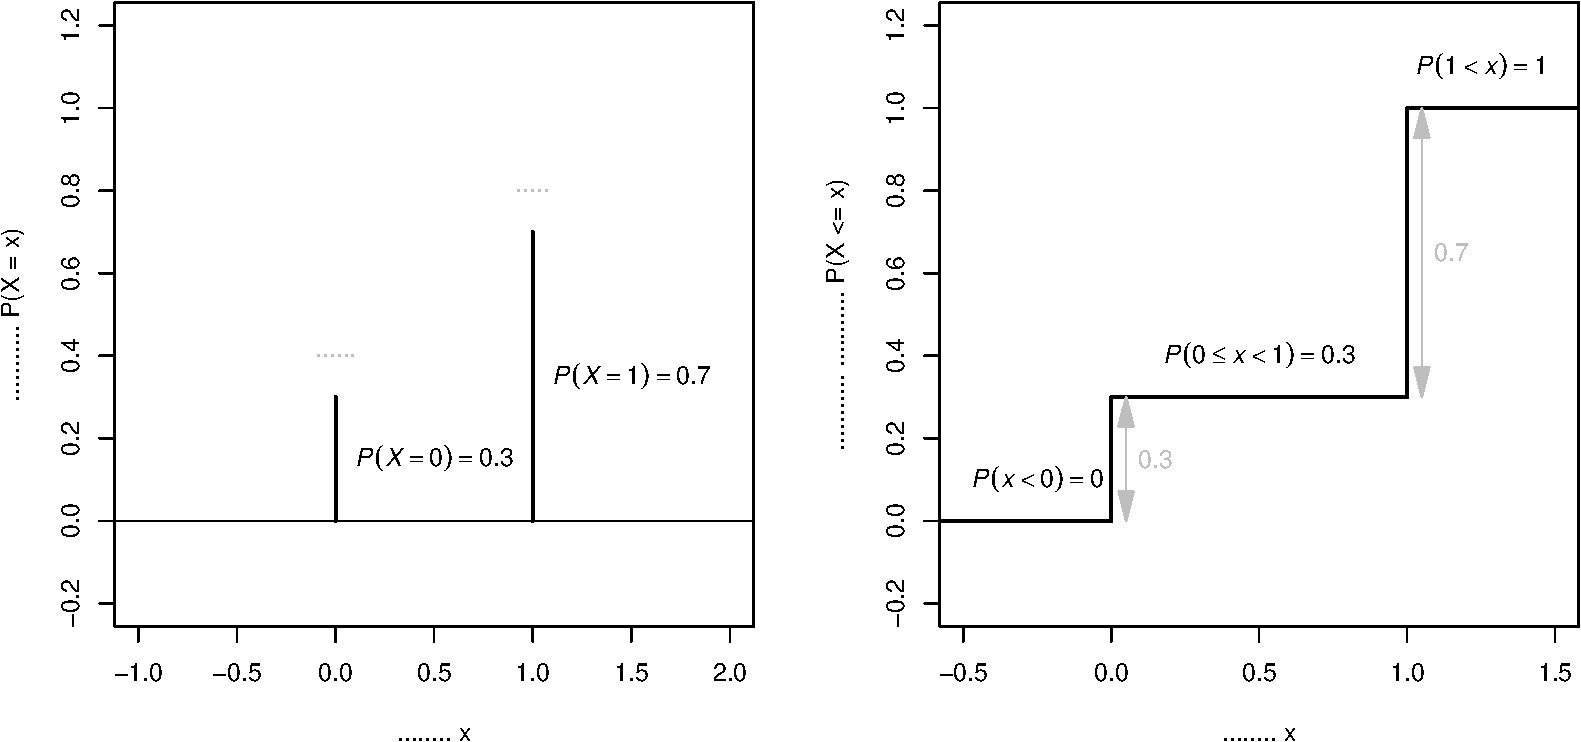
\includegraphics{bookdown-demo_files/figure-latex/fig-3-9-1.pdf}
\caption{\label{fig:fig-3-9}Функція маси ймовірності і функція кумулятивного розподілу для процесу Бернулі із \(p = 0.7\): елементарного підкидання монетки із \(70 \%\) ймовірністю випадіння аверсу.}
\end{figure}

Для дискретних змінних, pmf задана як \(f(x) = P(X = x) \forall x\) і \(P(X = u) = 0\) якщо \(u \notin \mathcal{X}\). Для трансформації pmf в cdf можна обчислити \(F(x) = P(X \leq x) = \sum \limits_{u: u \leq x} P(X = u) = \sum \limits_{u: u \leq x} f(u)\), а для протилежної трансформації cdf в pmf можна обчислити \(f(x) = F(u) - \lim \limits_{h \downarrow 0} F(u - h)\). Для неперервної ж змінної, \(f(u) = F(X = u) - \lim \limits_{h \downarrow 0} F(u - h) = 0\), адже \(P(X = u) = 0 \forall u\); cdf можна перевести в pdf як \(f(x) = \frac{d F(x)}{d x}\), і зворотньо pdf у cdf як \(F(x) = \int \limits_{u: u \leq x} f(u) du\).

Важливим параметром для опису будь-якої функції розподілу ймовірності є \textbf{математичне очікування, або математичне сподівання}. Для всякої функції \(f(x)\), математичне очікування можна знайти як середнє усіх можливих значень \(x: x \in \mathcal{X}\) зважене за ймовірністю цих значень \(f(x)\): відтак, для дискретних розподілів \(X\) математичне очікування змінної оціюється як \(\mathbb{E}[X] = \sum \limits_{x \in \mathcal{X}} x f(x)\), а для неперервних -- як \(\mathbb{E}[X] = \int \limits_{x \in \mathcal{X}} x f(x) dx\). Подібно до очікування змінної, можна шукати й очікування функції змінної \(g(x)\): \(\mathbb{E}[g(X)] = \sum \limits_{x \in \mathcal{X}} g(x) f(x)\) або \(\mathbb{E}[g(X)] = \int \limits_{x \in \mathcal{X}} g(x) f(x) dx\). Якщо очікування існує (є такі функції, для яких неможливо аналітично вирішити суми чи інтеграли), воно матиме наступні властивості:

\begin{itemize}
\item
  якщо \(c\) константа, то \(\mathbb{E}[c] = c\),
\item
  якщо \(c\) константа і \(g()\) -- функція, то \(\mathbb{E}[c g(X)] = c \mathbb{E} [g(X)]\),
\item
  якщо \(c_1\) та \(c_2\) є константами і \(g_1()\), \(g_2()\) -- функціями, то \(\mathbb{E}[c_1 g_1 (X) + c_2 g_2(X)] = c_1 \mathbb{E}[g_1(X)] + c_2 \mathbb{E}[g_2(X)]\).
\end{itemize}

Математичне очікування змінної \(\mathbb{E}[X]\) ще часто називають \textbf{середнім} (не плутати із середнім арифметичним, яке є середнім для нормального розподілу і деяких інших розподілів). Іншим важливим окремим випадком математичного очікування функції розподілу її ймовірності є її \textbf{варіація} \(Var[X]\) -- очікування середньоквадратичного відхилення випадкової змінної від її середнього:

\[
\begin{aligned}
  Var[X] = \mathbb{E} \left[ (X - \mathbb{E}[X])^2 \right] = \mathbb{E} \left[ X^2 - 2X \mathbb{E} [X] + (\mathbb{E} [X])^2 \right] = \\
  \mathbb{E} [X^2] - 2 \mathbb{E}[X] \mathbb{E}[X] + (\mathbb{E}[X])^2 = \mathbb{E} [X^2] - 2 \mathbb{E}[X] \mathbb{E}[X] + \mathbb{E}[X] \mathbb{E}[X] = \\
  \mathbb{E}[X^2] - \mathbb{E}[X] \mathbb{E}[X] = \mathbb{E}[X^2] - (\mathbb{E}[X])^2
\end{aligned}
\]

Функції розподілу ймовірності можуть приймати будь-який вигляд\footnote{особливо pdf: часто значення функції перевищує одиницю, що викликає справедливе питання ``а як ймовірність може бути більша за одиницю?''. Не може, але й ця функція не повертає ймовірність. Її \emph{інтеграл} повертає ймовірність.}. Розгляньмо окремі випадки поширених розподілів ймовірності. В усіх випадках ми кажемо що випадкова змінна \(X\) походить із певного розподілу \(f(x)\) позначенням \(X \sim \mathcal{A}(\theta, \cdots)\) де \(\theta\) є параметром розподілу \(\mathcal{A}\).

Нижче наведено формули розподілів ймовірності і, якщо доцільно, кумулятивних розподілів для окремих поширених статистичних розподілів. Також наведено значення середнього та варіації цих розподілів з точки зору параметрів і наявні шляхи обчислення \emph{оцінки} параметрів (позначені як \(\hat{\theta}\) для параметру \(\theta\)) для вибірки \(x_i \in X\) розміром \(n\) \footnote{варто зауважити, що формули оцінщиків взяті із відкритих джерел, включно із постами блогів. Кожен розподіл має своєрідну ситуацію із оцінщиками, і виведення оцінщиків не завжди проводиться методом максимальної правдоподібності чи за допомогою момент-генеруючих функцій (ми не торкаємось цього методу), ба того, такі оцінщики іноді є упередженими (biased). Використовувати оцінщики параметрів необхідно із застереженнями!}.

\subsubsection{Дискретні розподіли}\label{ux434ux438ux441ux43aux440ux435ux442ux43dux456-ux440ux43eux437ux43fux43eux434ux456ux43bux438}

\paragraph{Розподіл Бернулі}\label{ux440ux43eux437ux43fux43eux434ux456ux43b-ux431ux435ux440ux43dux443ux43bux456}

Розподіл Бернулі описує дискретну змінну із лише двома класами, відтак, яку можна представити як бінарну змінну: \(x \in \mathcal{X}: \mathcal{X} = \{0, 1\}\). Прикладом слугує підкидання монетки.

\begin{itemize}
\item
  Позначення: \(X \sim \mathcal{Bernoulli}(p)\)
\item
  pmf: \(f(x) = P(X = x) = p^x (1-p)^{x-1}\),
\item
  cdf: \(F(x) = P(X \leq x) = 0 \mathbb{I}_x(x < 0)\), \(P(X \leq x) = (1 - p) \mathbb{I}_x(0 \leq x < 1)\), \(P(X \leq x) = 1 \mathbb{I}_x(1 < x)\).
\item
  середнє \(\mathbb{E} [X] = \frac{N+1}{2} = p\),
\item
  варіація \(Var[X] = p(1 - p)\),
\item
  оцінщик \(\hat{p} = \frac{1}{n} \sum \limits_{i=1}^{n}x_i\).
\end{itemize}

\paragraph{Дискретний рівномірний розподіл}\label{ux434ux438ux441ux43aux440ux435ux442ux43dux438ux439-ux440ux456ux432ux43dux43eux43cux456ux440ux43dux438ux439-ux440ux43eux437ux43fux43eux434ux456ux43b}

Дискретний рівномірний розподіл описує ситуацію, в якій кожна із дискретних величин (\(\mathcal{X} = \{1, 2, 3, \cdots, N\}\)) має однакову ймовірність потрапити у вибірку. Прикладом можуть слугувати гральні кісточки.

\begin{itemize}
\item
  Позначення: \(X \sim \mathcal{DU}(N)\) або \(X \sim \mathcal{DU}(a, b)\) де \(N = b - a + 1 \text { } \forall b \geq a\),
\item
  pmf: \(f(x) = P(X = x) = \frac{1}{N} \mathbb{I}_x (x \in \{0, 1, 2, 3, \cdots, N\})\),
\item
  cdf: \(F(x) = P(X \leq x) = \frac{x - a + 1}{N}\),
\item
  середнє \(\mathbb{E} [X] = \frac{N+1}{2} = \frac{a+b}{2}\),
\item
  варіація \(Var[X] = \frac{N^2 - 1}{12}\),
\item
  оцінщик \(\hat{N} = \frac{n+1}{n} \max (x_i)\).
\end{itemize}

\paragraph{Біноміальний розподіл}\label{ux431ux456ux43dux43eux43cux456ux430ux43bux44cux43dux438ux439-ux440ux43eux437ux43fux43eux434ux456ux43b}

Проведіть \(n\) незалежних випадкових експериментів Бернулі: \(X \sim \mathcal{Bernoulli}(p)\). Якщо позначити \(y\) як кількість успішних експериментів в \(X\) із \(n\) спроб, то \(Y\) описуватиметься біноміальним розподілом.

\begin{itemize}
\item
  Позначення: \(Y \sim \mathcal{Binomial}(n, p)\),
\item
  pmf: \(f(Y) = P(Y = y) = \binom{n}{y} p^y (1-p)^{n - y} \mathbb{I}_y (y \in \{0, 1, 2, \cdots, n\})\)\footnote{cdf біноміального розподілу існує, але його складно вивести і він все одно мало що скаже; варіацію біноміального розподілу також шукати відносно непросто.},
\item
  середнє \(\mathbb{E} [Y] = np\) \footnote{обчислення очікування із біноміальними коефіцієнтами включає розкладання біному: \((a + b)^n = \sum \limits_{x = 0}^n \binom{n}{x} a^x b^{n - x}\)},
\item
  варіація \(Var[Y] = np(1-p)\),
\item
  оцінщик \(\hat{p} = \frac{y}{n}\).
\end{itemize}

\paragraph{Геометричний розподіл}\label{ux433ux435ux43eux43cux435ux442ux440ux438ux447ux43dux438ux439-ux440ux43eux437ux43fux43eux434ux456ux43b}

Уявіть повторення випадкового експерименту Бернулі із параметром \(p\) до того, поки не випаде перший успіх. В такому випадку, можна розрахувати кількість безуспішних спроб \(x\) до першого успіху та кількість спроб \(y\) потрібних для першого успіху. Обидві змінні описуються геометричним розподілом.

\begin{itemize}
\tightlist
\item
  pmf:
\end{itemize}

\[f(x) = P(X = x) = p(1 - p)^x \mathbb{I}_x (0, 1, 2, \cdots, \infty)\]

\[f(y) = P(Y = y) = p(1-p)^{y-1} \mathbb{I}_y (0, 1, 2, \cdots, \infty)\]

\begin{itemize}
\tightlist
\item
  середні
\end{itemize}

\[\mathbb{E} [X] = \frac{1-p}{p}\]

\[\mathbb{E} [Y] = \frac{1}{p}\]

\begin{itemize}
\tightlist
\item
  варіації
\end{itemize}

\[Var[X] = \frac{1-p}{p^2}\]

\[Var[Y] = \frac{1-p}{p^2}\]

\begin{itemize}
\tightlist
\item
  оцінщик \(\hat{p} = \frac{1}{x}\).
\end{itemize}

\paragraph{Негативний біноміальний розподіл}\label{ux43dux435ux433ux430ux442ux438ux432ux43dux438ux439-ux431ux456ux43dux43eux43cux456ux430ux43bux44cux43dux438ux439-ux440ux43eux437ux43fux43eux434ux456ux43b}

Негативний біноміальний розподіл описує \(X\) як кількість невдач перед \(r\)-тим успіхом в серії випадкових експериментів Бернулі із параметром \(p\).

\begin{itemize}
\item
  Позначення: \(X \sim \mathcal{NBinom} (r, p)\),
\item
  pmf: \(f(x) = P(X = x) = \binom{\text{спроби}}{\text{успіхи} + x \text{ невдач}} \cdot \text{невдачі} \cdot \text{успіхи} = \binom{x + r - 1}{r-1} (1-p) ^x p^r\),
\item
  середнє \(\mathbb{E} [X] = \frac{r(1-p)}{p}\),
\item
  варіація \(Var[X] = \frac{r(1-p)}{p^2}\),
\item
  оцінщик \(\hat{p} = \frac{r-1}{r + x - 1}\).
\end{itemize}

Примітно, що геометричний розподіл є окремим випадком негативного біноміального розподілу. Якщо \(Y\) -- кількість спроб для отримання \(r\) успіхів, то \(Y = X + r\), \(P(Y = y) = \binom{y-1}{r-1} (1-p)^{y-r} p^r\). \(\mathbb{E}[Y] = \mathbb{E}[X] + r\), \(Var[Y] = Var[X]\).

\paragraph{Розподіл Пуасона}\label{ux440ux43eux437ux43fux43eux434ux456ux43b-ux43fux443ux430ux441ux43eux43dux430}

Мабуть, один із найменш інтуїтивно зрозумілих але найбільш поширених розподілів. Він описує кількість подій, які відбуваються протягом визначеного вікна в просторі, при тому що всі події є незалежними один від одного. Існує чимало прикладів процесів Пуасона, наприклад, кількість людей на платформі залізничної станції в момент часу чи кількість особин популяції зареєстрованих на ділянці.

\begin{itemize}
\item
  Позначення: \(X \sim \mathcal{Poisson}(\lambda)\)
\item
  pmf: \(f(x) = P(X = x) = e^{-\lambda} \frac{\lambda^x}{x!}\), де \(x \in \{0, 1, 2, 3, \cdots, \infty \}\), \(\lambda > 0\),
\item
  середнє \(\mathbb{E} [X] = \lambda\),
\item
  варіація \(Var[X] = \lambda\),
\item
  оцінщик \(\hat{\lambda} = \frac{1}{n} \sum \limits_{i=1}^{n}x_i\).
\end{itemize}

Цікаво, що \(Y \sim \mathcal{Binomial}(n, p)\) із не-екстремальним значенням \((np)\) та дуже значним \(n\) може бути апроксимована до розподілу Пуасона із \(\lambda \approx np\).

\paragraph{Гіпергеометричний розподіл}\label{ux433ux456ux43fux435ux440ux433ux435ux43eux43cux435ux442ux440ux438ux447ux43dux438ux439-ux440ux43eux437ux43fux43eux434ux456ux43b}

Уявіть зліченну популяцію розміром \(N\) із об'єктів, що належать до різних класів, зокрема, в якій існує \(K: K \leq N\) об'єктів із певною характеристикою (наприклад, особини виду, в якому ми зацікавлені, в угрупованні різних видів\footnote{застосування гіпергеометричного розподілу в реальних задачах екології угруповань може бути складним, адже чисельності видів можуть сягати сотень і тисяч, й обчислення біноміальних коефіцієнтів видасть дуже великі числа -- іноді настільки великі, що комп'ютер не може їх обчислити і зве безкінечністю. Аби обійти обмеження стандартної комп'ютерної архітектури в нагоді можуть стати функції із бібліотеки \texttt{gmp} для R.}). Тоді можна очікувати, що вибірка розміром \(n\) із цілої популяції міститиме \(x\) об'єктів із шуканого класу.

\begin{itemize}
\item
  Позначення: \(X \sim \mathcal{HyperGeom}(N, K, n)\),
\item
  pmf: \(f(x) = P(X = x) = \frac{\binom{N}{K} \binom{N-K}{n - x}}{\binom{N}{n}}\),
\item
  середнє \(\mathbb{E} [X] = n \frac{K}{N}\),
\item
  оцінщик для \href{https://math.stackexchange.com/questions/40319/maximum-likelihood-estimate-of-hypergeometric-distribution-parameter}{випадків апроксимації до розподілу Пуасона} де \(K/N << 1, n >> 1\): \(\hat{m} = \frac{N \sum \limits_i^T x_i}{Tn}\) для вибірки \(x_i \in X\) розміром \(T\).
\end{itemize}

\subsubsection{Континуальні розподіли}\label{ux43aux43eux43dux442ux438ux43dux443ux430ux43bux44cux43dux456-ux440ux43eux437ux43fux43eux434ux456ux43bux438}

\paragraph{Рівномірний розподіл}\label{ux440ux456ux432ux43dux43eux43cux456ux440ux43dux438ux439-ux440ux43eux437ux43fux43eux434ux456ux43b}

Рівномірний розподіл описує ситуацію, коли будь-яке значення \(x\) між \(a\) і \(b\) має рівну ймовірність: \(P(a \leq X \leq b) = 1\).

\begin{itemize}
\item
  Позначення: \(X \sim \mathcal{U}(a, b)\),
\item
  pdf: \(f(x) = \frac{1}{b-a} \mathbb{I}_x (a \leq x \leq b)\) (примітно, що функція є константою),
\item
  cdf: \(F(x) = P(X \leq x) = \frac{x-a}{b-a} \text { } \forall (a \leq x \leq b)\), але \(F(X) = 0 \mathbb{I}_x(x < 0)\) і \(F(X) = 1 \mathbb{I}_x (1 < x)\),
\item
  середнє \(\mathbb{E} [X] = \frac{a+b}{2}\),
\item
  варіація \(Var[X] = \frac{(b-a)^2}{12}\),
\item
  оцінщики \(\hat{a} = \min(x_i), \hat{b} = \max(x_i)\).
\end{itemize}

\paragraph{Бета-розподіл}\label{ux431ux435ux442ux430-ux440ux43eux437ux43fux43eux434ux456ux43b}

Доволі різноманітна родина угпуповань із формою функції, яка контролюється двома параметрами, \(a\) і \(b\). Щодо цього розподілу, мабуть, варто просто знати про його існування. Його іноді застосовують в популяційній генетиці \href{https://doi.org/10.1007\%2FBF01441146}{(Balding \& Nichols 1995)} та Баєсівському аналізі \href{https://doi.org/10.1109/MFI.2016.7849531}{(Jøsang 2016)}.

\begin{itemize}
\item
  Позначення: \(X \sim \mathcal{Beta}(a, b)\),
\item
  pdf: \(f(x) \propto x^{a - 1} (1-x)^{b-1} \mathbb{I}_x(0 < x < 1)\), \(f(x) = \frac{\Gamma (a + b)}{\Gamma (a) \Gamma (b)} x^{a - 1} (1 - x)^{b - 1}\), де \(\Gamma()\) - гамма-функція \(\Gamma(\alpha) = \int \limits_0^{\infty} u^{\alpha - 1} e^{-u} du\).
\item
  середнє \(\mathbb{E} [X] = \frac{a}{a + b}\),
\item
  варіація \(Var[X] = \frac{ab}{(a+b)^2 (a+b+1)}\).
\end{itemize}

\paragraph{Експоненційний розподіл}\label{ux435ux43aux441ux43fux43eux43dux435ux43dux446ux456ux439ux43dux438ux439-ux440ux43eux437ux43fux43eux434ux456ux43b}

Експоненційний розподіл є своєрідним неперервним аналогом геометричного розподілу і описує відстань між незалежними неперервними подіями, які відбуваються із постійним темпом. Розподіл темпів смертності в природних популяціях нагадує експоненційний \href{https://doi.org/10.1016/0022-5193(79)90098-5}{(Abernethy 1979)}.

\begin{itemize}
\item
  Позначення: \(X \sim \mathcal{Exp}(\lambda)\),
\item
  pdf: \(f(x) = \frac{1}{\lambda} e^{-\frac{x}{\lambda}} \mathbb{I}_x (0 \leq x \leq \infty)\),
\item
  cdf: \(F(x) = 1 - e^{-\frac{x}{\lambda}}\),
\item
  середнє \(\mathbb{E} [X] = \lambda\),
\item
  варіація \(Var[X] = \lambda^2\),
\item
  оцінщик \(\hat{(\frac{1}{\lambda})} = \frac{1}{n} \sum x_i\) із упередженням, або \(\hat{(\frac{1}{\lambda})} = \frac{n-2}{\sum x_i}\).
\end{itemize}

Цікавою властивістю експоненційного процесу є відсутність пам'яті: ймовірність вижити в наступний момент часу за умови виживання до цього моменту дорівнює ймовірності вижити в будь-який момент часу (\(P(X > (s+t)|X > s) = P(X > t)\)).

Особливим випадком експоненційного розподілу є двопараметричний \textbf{зміщений експоненційний розподіл}: \(f(x) = \frac{1}{\lambda} e^{-\frac{x - \mu}{\lambda}} \mathbb{I}_x (\mu \leq x \leq \infty)\), для якого середнє дорівнює \(\mathbb{E}[X] = \mu + \lambda\).

\paragraph{Нормальний розподіл}\label{ux43dux43eux440ux43cux430ux43bux44cux43dux438ux439-ux440ux43eux437ux43fux43eux434ux456ux43b}

Мабуть, найбільш знаменитий розподіл, яким можна описати чимало змінних в біології: розміри листків рослин, зріст людей певного віку тощо. Його логіка доволі проста і каже що змінна \(X\) матиме значення \(x\), які концентруються навколо якогось середнього значення \(\bar{x}\), і чим сильніше \(x\) відрізняються від \(\bar{x}\), тим менш поширеними вони будуть. Цьому розподілу варто приділити дещо більше уваги, аніж іншим.

\begin{itemize}
\item
  Позначення: \(X \sim \mathcal{N}(\mu, \sigma^2)\), де параметр \(\mu: \{-\infty \leq \mu \leq \infty\}\) відповідає середньому значенню (а також \textbf{\emph{медіані}} \footnote{\textbf{медіана} -- значення в сортованій послідовності випадкової змінної \(X\), яке розділяє цю послідовність на дві частини однакового розміру; медіана тісно пов'язана із поняттями \textbf{перцентилів} \(x_{\alpha}\) -- такими значеннями \(x\), які більше за частку \(\alpha\) випадкової змінної \(X\) (наприклад, перцентиль \(x_{\alpha = 0.95}\) -- це таке значення, що в змінній \(X\) \(95 \%\) значень менше або дорівнюють \(x_{\alpha = 0.95}\)). Медіана відповідає перцентилю із \(\alpha = 0.5\).} та \textbf{\emph{моді}} \footnote{\textbf{мода} -- найбільш поширене значення у вибірці.}), а параметр \(\sigma^2: \sigma > 0\) відповідає варіації в розподілі, що виражається в ширині характерної куполоподібної кривої.
\item
  pdf: \(f(x) = \frac{1}{\sqrt{2 \pi} \sigma} e^{-\left[ \frac{(x - \mu)^2}{2 \sigma^2} \right]}\),
\item
  середнє \(\mathbb{E} [X] = \mu\),
\item
  варіація \(Var[X] = \sigma^2\).
\end{itemize}

Хорошою демонстрацією методу \hyperref[mle]{максимальної правдоподібності} є пошук параметрів із такої вибірки \(X\) що \(X \sim \mathcal{N}(\mu, \sigma^2)\). Знайдемо функцію правдоподібності:

\[\mathcal{L}(X | \mu, \sigma^2) = \prod \limits_{i=1}^n f(x_i| \mu, \sigma^2) = \prod \limits_{i=1}^n \frac{1}{\sqrt{2 \pi} \sigma} e^{-\left[ \frac{(x - \mu)^2}{2 \sigma^2} \right]} = \left( \frac{1}{\sqrt{2 \pi \sigma^2}} \right)^n \exp \left[ - \frac{\sum \limits_{i=1}^n (x_i - \mu)}{2 \sigma^2} \right]\]

Оскільки бавитись з такою формулою виглядає тією ще задачею, візьмемо логарифм правдоподібності:

\[\ln \mathcal{L}(X | \mu, \sigma^2) = - \frac{n}{2} \ln{(2 \pi \sigma^2)} - \frac{\sum \limits_{i=1}^n (x_i - \mu)}{2 \sigma^2}\]

Знайдемо оцінщик \(\hat{\mu}\) першим. Для цього потрібно продиференціювати попередній вираз відносно \(\mu\) і прирівняти його до нуля:

\[\frac{\partial \ln \mathcal{L}(X | \mu, \sigma^2)}{\partial \mu} = \frac{\sum \limits_{i=1}^n (x_i - \mu)}{\sigma^2} = 0\]
Відтак, рішення

\[\sum \limits_{i=1}^n (x_i - \mu) = 0 \Rightarrow \sum \limits_{i=1}^n x_i - n \mu = 0 \Rightarrow \hat{\mu} = \frac{\sum \limits_{i=1}^n x_i}{n}\]
Що ніщо інше як середнє арифметичне. Щодо іншого параметру, \(\sigma^2\),

\[\frac{\partial \ln \mathcal{L}(X | \mu, \sigma^2)}{\partial \sigma^2} = - \frac{n}{2} \cdot \frac{2 \pi}{2 \pi \sigma^2} + \frac{\sum \limits_{i=1}^n (x_i - \mu)^2}{2 (\sigma^2)^2} = 0 \Rightarrow -n \sigma^2 + \sum \limits_{i=1}^n (x_i - \mu)^2 = 0\]

Можна підставити \(\hat{\mu} = \frac{1}{n} \sum \limits_{i=1}^n x_i = \bar{x}\) і отримати

\[\hat{\sigma^2} = \frac{1}{n} \sum \limits_{i=1}^n (x_i - \bar{x})^2\]

Якщо читач дещо обізнаний в базовій статистиці, то можна помітити що цією формулою \emph{не} користуються для оцінки дисперсії у вибірках із нормального розподілу. Все через те, що такий оцінщик не проходить перевірку на упередженість (bias: оцінщик вважається неупередженим якщо \(\mathbb{E}[\hat{\theta}] = \theta\)): якщо переформулювати (подано без покрокових обчислень, можна перевірити якщо пам'ятати що \(\frac{1}{n} \sum \limits_{i=1}^n x_i \equiv \bar{x}\))

\[\hat{\sigma^2} = \frac{1}{n} \sum \limits_{i=1}^n (x_i - \bar{x})^2 = \frac{1}{n} \sum \limits_{i=1}^n x_i^2 - (\bar{x})^2\]

Тоді (пам'ятаючи що \(\sigma^2 = Var[X] = \mathbb{E} [X^2] - (\mathbb{E} [X])^2 = \mathbb{E} [X^2] - \mu^2\))

\[\mathbb{E} [\hat{\sigma^2}] = \mathbb{E} \left[ \frac{1}{n} \sum \limits_{i=1}^n x_i^2 - (\bar{x})^2 \right] = \frac{1}{n} \sum \limits_{i = 1}^n \mathbb{E} [x_i^2] - \mathbb{E} [\bar{x}^2] = \frac{1}{n}  \sum \limits_{i = 1}^n (\sigma^2 + \mu^2) - (\frac{\sigma^2}{n} + \mu^2) = (1 - \frac{1}{n}) \sigma^2 \neq \sigma^2\]

Натомість, неупередженим оцінщиком \(\hat{\sigma^2}\) є щось, що називають \textbf{дисперсією вибірки}: \(\hat{\sigma^2} = s^2 = \frac{1}{n-1} \sum \limits_{i=1}^n (x_i - \bar{x})^2\). Аби уникнути термінологічної плутанини (а вона чомусь завжди наявна в оцінках варіації), варто визначити наступні дескриптори варіації, що часто застосовуються до вибірок із нормальним розподілом (використовуйте тест Шапіро-Вілка (Shapiro-Wilk test) для перевірки нормальності вибірки; \(p > 0.05\), на відміну від більшості статистичних тестів, є підставою вважати вибірку нормально розподіленою):

\begin{itemize}
\item
  \textbf{\emph{дисперсія}} (sample variance) є неупередженим оцінщиком параметру нормального розподілу у вибірці: \(s^2 = \frac{1}{n-1} \sum \limits_{i=1}^n (x_i - \bar{x})^2\),
\item
  \textbf{\emph{середньоквадратичне відхилення}}, або \textbf{\emph{стандартне відхилення}} (standard deviation, SD) описує варіацію вибірки незалежно від її розподілу: \(v = \frac{1}{n} \sum \limits_{i=1}^n (x_i - \bar{x})^2\),
\item
  \textbf{\emph{стандартна помилка}} (standard error, SE) описує відхилення вибіркового середнього \(\bar{x}\): \(\frac{s}{\sqrt{n}}\).
\end{itemize}

Щодо важливості нормального розподілу в статистиці, варто згадати закон великих чисел та центральну граничну теорему. \textbf{Закон великих чисел} стверджує, що якщо із \textbf{\emph{генеральної сукупності}} \footnote{\textbf{генеральна сукупність} -- поширене поняття в статистиці; якщо спостерігач обрав вибірку значень (наприклад, вага особин модельного виду), ця вибірка є лише обмеженою підмножиною генеральної сукупності, розмір якої апроксимує до безкінечності. Ми припускаємо що вибірка є репрезентативною щодо генеральної сукупності, отже, розподіл ймовірності в генеральній сукупності апроксимує до розподілу в генеральній сукупності. Неможливо набрати вибірку розміром із розмір генеральної сукупності -- спостерігач завжди пропустить бодай один зразок.} незалежно і багаторазово набирати окремі вибірки, то усереднена статистика\footnote{статистика - інше слово для параметру вибірки. Середнє арифметичне є статистикою, дисперсія є статистикою тощо} цих вибірок наближається до істинного значення статистики генеральної сукупності, якщо таке існує. В контексті нормального розподілу, середні вибірок (\(\hat{\mu}\)) з генеральної сукупності конвергують до середнього генеральної сукупності \(\mu\). \textbf{Центральна гранична теорема} ж постулює, що в множині таких незалежних \emph{змінних} \(X_1, X_2, X_3, \cdots, X_n\), що \(\mathbb{E} [X_i] = \mu\), \(Var[X_i] = \sigma^2\), незалежно від розподілу окремих змінних \(X_i\), за \(n \rightarrow \infty\) розподіл змінних \(\sqrt{n} (\frac{1}{n}\sum \limits_{i=1}^n X_i - \mu)\) конвергує до \(\mathcal{N}(0,  \sigma^2)\). Іншими словами, яким би не був розподіл генеральної сукупності, розподіл середніх значень вибірок із такої генеральної сукупності буде нагадувати нормальний розподіл.

\paragraph{Лог-нормальний розподіл}\label{ux43bux43eux433-ux43dux43eux440ux43cux430ux43bux44cux43dux438ux439-ux440ux43eux437ux43fux43eux434ux456ux43b}

Змінна \(X\) розподілена лог-нормально (\(X \sim L\mathcal{N}(\mu, \sigma^2)\)) якщо \(\ln(X) \sim \mathcal{N}(\mu, \sigma^2)\). Відтак, якщо поглянути з іншого боку, то якщо \(Y \sim \mathcal{N}(\mu, \sigma^2)\), то \(X = e^Y \sim L\mathcal{N}(\mu, \sigma^2)\).

\begin{itemize}
\item
  Середнє \(\mathbb{E} [\ln (X)] = \mu, \mathbb{E}[X] = e^{\mu + \frac{\sigma^2}{2}}\),
\item
  варіація \(Var[\ln(X)] = \sigma^2, Var[X] = \exp [2(\mu - \sigma^2)] - \exp [2 \mu + \sigma^2]\).
\end{itemize}

\paragraph{Розподіл Коші}\label{ux440ux43eux437ux43fux43eux434ux456ux43b-ux43aux43eux448ux456}

Доволі дивний розподіл, який формою нагадує нормальний із набагато гострішим піком та товстішими хвостами.

\begin{itemize}
\item
  Позначення: \(X \sim \mathcal{Cauchy}(x_0, \gamma)\), де \(\gamma\) регулює форму кривої, а \(x_0\) відповідає локації піку.
\item
  pdf: \(f(x) = \frac{1}{\pi} \left[ \frac{\gamma}{(x - x_0)^2 + \gamma^2} \right]\)
\end{itemize}

Дивність цього розподілу полягає в тому, що його середнє й варіація неможливо аналітично визначити. Оцінки середнього арифметичного і cередньоквадратичного відхилення не конвергують зі збільшенням розміру вибірки, а єдиним більш-менш точним методом оцінки параметру форми \(\hat{\gamma}\) є медіана абсолютних значень вибірки.

\subsection{Опис розподілу змінної}\label{ux43eux43fux438ux441-ux440ux43eux437ux43fux43eux434ux456ux43bux443-ux437ux43cux456ux43dux43dux43eux457}

\subsection{Статистична гіпотеза}\label{ux441ux442ux430ux442ux438ux441ux442ux438ux447ux43dux430-ux433ux456ux43fux43eux442ux435ux437ux430}

\subsection{Нульовий розподіл}\label{ux43dux443ux43bux44cux43eux432ux438ux439-ux440ux43eux437ux43fux43eux434ux456ux43b}

\subsection{Тестування гіпотез}\label{ux442ux435ux441ux442ux443ux432ux430ux43dux43dux44f-ux433ux456ux43fux43eux442ux435ux437}

\subsection{Парадигми статистичного аналізу}\label{paradigms}

\subsection{Псевдореплікація}\label{ux43fux441ux435ux432ux434ux43eux440ux435ux43fux43bux456ux43aux430ux446ux456ux44f}

\subsection{Проблема регресії і проблема класифікації}\label{ux43fux440ux43eux431ux43bux435ux43cux430-ux440ux435ux433ux440ux435ux441ux456ux457-ux456-ux43fux440ux43eux431ux43bux435ux43cux430-ux43aux43bux430ux441ux438ux444ux456ux43aux430ux446ux456ux457}

\subsection{Статистичний умомвивід і обґрунтоване передбачення}\label{ux441ux442ux430ux442ux438ux441ux442ux438ux447ux43dux438ux439-ux443ux43cux43eux43cux432ux438ux432ux456ux434-ux456-ux43eux431ux491ux440ux443ux43dux442ux43eux432ux430ux43dux435-ux43fux435ux440ux435ux434ux431ux430ux447ux435ux43dux43dux44f}

\subsection{Крос-валідація}\label{ux43aux440ux43eux441-ux432ux430ux43bux456ux434ux430ux446ux456ux44f}

\chapter{Початки популяційної екології}\label{popeco}

\section{Вид}\label{species}

\section{Популяція}\label{population}

\section{Метапопуляція}\label{metapopulation}

\section{Чинники, що впливають на популяції}\label{pop-factors}

\section{Внутрішньовидові взаємодії}\label{intraspecific}

\section{Динаміка та стабільність}\label{pop-dynamics}

\section{Матриці Леслі}\label{Leslie-matrix}

\chapter{Фундаментальні поняття екології}\label{foundations}

\section{Екологічна ніша}\label{niche}

\section{Трофічні ланцюги}\label{food-chain}

\section{Трофічні мережі}\label{food-webs}

\section{Ключові види}\label{keystones}

\section{Сукцесія та клімакс}\label{succession}

\section{Історія життя}\label{life-history}

\section{Ймовірність детекції}\label{detectability}

\chapter{Міжвидові взаємодії}\label{interspecific}

\section{Типи міжвидових зв'язків}\label{relationships}

\section{Теорія поділу ресурсів}\label{rstar}

\section{Трофічні каскади}\label{cascade}

\chapter{Екологічні угруповання}\label{comecol}

\section{Структура угруповання}\label{sad}

\section{Моделі розподілів чисельності}\label{sad-model}

\section{Різноманіття}\label{diversity}

\section{Функціональне й філогенетичне різноманіття}\label{fd}

\section{Острівна біогеографія}\label{islands}

\section{Середовищне фільтрування}\label{env-filter}

\section{Рарефакція та екстраполяція}\label{rarefaction}

\chapter*{Післяслово}\label{ux43fux456ux441ux43bux44fux441ux43bux43eux432ux43e}
\addcontentsline{toc}{chapter}{Післяслово}

\chapter*{Контакти автора}\label{ux43aux43eux43dux442ux430ux43aux442ux438-ux430ux432ux442ux43eux440ux430}
\addcontentsline{toc}{chapter}{Контакти автора}

Найкращий спосіб -- електронна пошта \href{mailto:oadubovyk@gmail.com}{\nolinkurl{oadubovyk@gmail.com}}

Листи невимовного захвату вкриті нестримними сльозами радості від читання посібника надсилати за адресою:

Oleksii Dubovyk, PhD Student

Dept Biol Sci, Mills Godwin Bldg 110

Old Dominion University, Norfolk, VA

23529, USA

  \bibliography{book.bib,packages.bib}

\end{document}
